%%____________________________________________________________________________||
\section{Results}
\label{app:results}

\subsection{Tabulated presentation of pre-fit result (signal and
  control regions)}
\label{app:results-tables-pre}

\subsubsection{Signal region}

\begin{table}[!h]
  \topcaption{
    Observed data counts and pre-fit background expectations in
    the signal region for the \texttt{eq1j} topology. The
    uncertainties in the background expectations include statistical
    contributions from the finite-sized simulation samples {\it only}. 
  }
  \label{tab:result-eq1j}
  \scriptsize
  \centering
  \begin{tabular}{rrlrrcl}
    \hline
    \njet\T\B & \nb & \scalht [GeV] & Data & \multicolumn{3}{c}{SM} \\ 
    \hline
1\T & 0 & $ 200- 400$ & 291353 & 254856.1 &$\pm$&  371.9 \\
1\T & 0 & $ 400- 600$ &   8572 &   7342.2 &$\pm$&   28.8 \\
1\T & 0 & $ 600- 900$ &    878 &    680.1 &$\pm$&    4.0 \\
1\T & 0 & $ 900- \infty$ &     57 &     56.9 &$\pm$&    0.9 \\
1\T & 1 & $ 200- 400$ &  11072 &   8864.3 &$\pm$&   27.4 \\
1\T & 1 & $ 400- 600$ &    406 &    334.6 &$\pm$&    2.7 \\
1\T & 1 & $ 600- \infty$ &     71 &     41.5 &$\pm$&    0.4 \\
    \hline
  \end{tabular}
\end{table}

\begin{table}[!h]
  \topcaption{
    Observed data counts and pre-fit background expectations in
    the signal region for the \texttt{ge2a} topology. The
    uncertainties in the background expectations include statistical
    contributions from the finite-sized simulation samples {\it only}. 
  }
  \label{tab:result-ge2a}
  \scriptsize
  \centering
  \begin{tabular}{rrllrrcl}
    \hline
    \njet\T\B & \nb & \scalht [GeV] & \mht [GeV] & Data & \multicolumn{3}{c}{SM} \\ 
    \hline
$\geq 2${\it a}\T & 0 & $ 200- 400$ & $200-\infty$ & 116868 & 101411.4 &$\pm$&  749.9 \\
$\geq 2${\it a}\T & 0 & $ 400- 600$ & $200-400$ &   2932 &   2909.4 &$\pm$&   20.6 \\
$\geq 2${\it a} & 0 & $ 400- 600$ & $400-\infty$ &   2800 &   2582.2 &$\pm$&   17.6 \\
$\geq 2${\it a}\T & 0 & $ 600- 900$ & $200-400$ &     31 &     22.7 &$\pm$&    1.0 \\
$\geq 2${\it a} & 0 & $ 600- 900$ & $400-600$ &     75 &     63.8 &$\pm$&    1.2 \\
$\geq 2${\it a} & 0 & $ 600- 900$ & $600-\infty$ &    211 &    198.9 &$\pm$&    2.0 \\
$\geq 2${\it a}\T & 0 & $ 900- \infty$ & $200-900$ &     28 &     31.8 &$\pm$&    0.8 \\
$\geq 2${\it a} & 0 & $ 900- \infty$ & $900-\infty$ &     54 &     50.3 &$\pm$&    0.8 \\
$\geq 2${\it a}\T & 1 & $ 200- 400$ & $200-\infty$ &  16307 &  13333.6 &$\pm$&  100.1 \\
$\geq 2${\it a}\T & 1 & $ 400- 600$ & $200-400$ &   1042 &    969.1 &$\pm$&    7.3 \\
$\geq 2${\it a} & 1 & $ 400- 600$ & $400-\infty$ &    310 &    275.8 &$\pm$&    3.2 \\
$\geq 2${\it a}\T & 1 & $ 600- 900$ & $200-400$ &      8 &     13.7 &$\pm$&    0.7 \\
$\geq 2${\it a} & 1 & $ 600- 900$ & $400-600$ &     12 &     11.4 &$\pm$&    0.4 \\
$\geq 2${\it a} & 1 & $ 600- 900$ & $600-\infty$ &     26 &     21.5 &$\pm$&    0.4 \\
$\geq 2${\it a}\T & 1 & $ 900- \infty$ & $200-900$ &      5 &      3.9 &$\pm$&    0.2 \\
$\geq 2${\it a} & 1 & $ 900- \infty$ & $900-\infty$ &      7 &      6.3 &$\pm$&    0.2 \\
$\geq 2${\it a}\T & 2 & $ 200- 400$ & $200-\infty$ &   2200 &   1856.5 &$\pm$&   18.0 \\
$\geq 2${\it a}\T & 2 & $ 400- 600$ & $200-400$ &    410 &    373.9 &$\pm$&    4.1 \\
$\geq 2${\it a} & 2 & $ 400- 600$ & $400-\infty$ &     35 &     23.9 &$\pm$&    0.8 \\
$\geq 2${\it a}\T & 2 & $ 600- 900$ & $200-400$ &      4 &      5.9 &$\pm$&    0.4 \\
$\geq 2${\it a} & 2 & $ 600- 900$ & $400-600$ &      4 &      2.3 &$\pm$&    0.2 \\
$\geq 2${\it a} & 2 & $ 600- 900$ & $600-\infty$ &      2 &      1.7 &$\pm$&    0.1 \\
$\geq 2${\it a}\T & 2 & $ 900- \infty$ & $200-900$ &      1 &      0.6 &$\pm$&    0.1 \\
$\geq 2${\it a} & 2 & $ 900- \infty$ & $900-\infty$ &      0 &      0.4 &$\pm$&    0.0 \\
$\geq 2${\it a}\T & 3 & $ 200- 400$ & $200-\infty$ &     92 &     70.7 &$\pm$&    1.1 \\
$\geq 2${\it a}\T & 3 & $ 400- 600$ & $200-400$ &     38 &     34.4 &$\pm$&    0.6 \\
$\geq 2${\it a} & 3 & $ 400- 600$ & $400-\infty$ &      2 &      0.6 &$\pm$&    0.1 \\
$\geq 2${\it a}\T & 3 & $ 600- \infty$ & $200-400$ &      1 &      0.9 &$\pm$&    0.1 \\
$\geq 2${\it a} & 3 & $ 600- \infty$ & $400-600$ &      0 &      0.2 &$\pm$&    0.0 \\
$\geq 2${\it a} & 3 & $ 600- \infty$ & $600-\infty$ &      0 &      0.1 &$\pm$&    0.0 \\
    \hline
  \end{tabular}
\end{table}

\begin{table}[!h]
  \topcaption{
    Observed data counts and pre-fit background expectations in
    the signal region for the \texttt{eq2j} topology. The
    uncertainties in the background expectations include statistical
    contributions from the finite-sized simulation samples {\it only}. 
  }
  \label{tab:result-eq2j}
  \scriptsize
  \centering
  \begin{tabular}{rrllrrcl}
    \hline
    \njet\T\B & \nb & \scalht [GeV] & \mht [GeV] & Data & \multicolumn{3}{c}{SM} \\ 
    \hline
2\T & 0 & $ 200- 400$ & $200-\infty$ &  34934 &  29224.5 &$\pm$&  144.9 \\
2\T & 0 & $ 400- 600$ & $200-400$ &   3468 &   3274.3 &$\pm$&   76.2 \\
2 & 0 & $ 400- 600$ & $400-\infty$ &   2568 &   2176.9 &$\pm$&   48.6 \\
2\T & 0 & $ 600- 900$ & $200-400$ &    226 &    276.7 &$\pm$&    6.9 \\
2 & 0 & $ 600- 900$ & $400-600$ &    253 &    268.4 &$\pm$&    6.6 \\
2 & 0 & $ 600- 900$ & $600-\infty$ &    303 &    284.6 &$\pm$&    6.6 \\
2\T & 0 & $ 900-1200$ & $200-400$ &    165 &    179.3 &$\pm$&    2.4 \\
2 & 0 & $ 900-1200$ & $400-600$ &    125 &    130.9 &$\pm$&    2.0 \\
2 & 0 & $ 900-1200$ & $600-900$ &     97 &     78.7 &$\pm$&    1.4 \\
2 & 0 & $ 900-1200$ & $900-\infty$ &     25 &     29.3 &$\pm$&    0.8 \\
2\T & 0 & $1200- \infty$ & $200-400$ &      9 &     11.8 &$\pm$&    0.5 \\
2 & 0 & $1200- \infty$ & $400-600$ &     26 &     33.4 &$\pm$&    0.8 \\
2 & 0 & $1200- \infty$ & $600-900$ &     22 &     28.0 &$\pm$&    0.7 \\
2 & 0 & $1200- \infty$ & $900-\infty$ &     19 &     20.9 &$\pm$&    0.5 \\
2\T & 1 & $ 200- 400$ & $200-\infty$ &   3850 &   3006.6 &$\pm$&   20.8 \\
2\T & 1 & $ 400- 600$ & $200-400$ &    327 &    277.4 &$\pm$&    6.9 \\
2 & 1 & $ 400- 600$ & $400-\infty$ &    240 &    219.3 &$\pm$&    5.4 \\
2\T & 1 & $ 600- 900$ & $200-400$ &     22 &     26.9 &$\pm$&    0.8 \\
2 & 1 & $ 600- 900$ & $400-600$ &     39 &     25.5 &$\pm$&    0.8 \\
2 & 1 & $ 600- 900$ & $600-\infty$ &     31 &     27.1 &$\pm$&    0.8 \\
2\T & 1 & $ 900-1200$ & $200-400$ &     17 &     19.3 &$\pm$&    0.4 \\
2 & 1 & $ 900-1200$ & $400-600$ &     15 &     14.9 &$\pm$&    0.4 \\
2 & 1 & $ 900-1200$ & $600-900$ &     12 &      7.4 &$\pm$&    0.2 \\
2 & 1 & $ 900-1200$ & $900-\infty$ &      6 &      3.2 &$\pm$&    0.1 \\
2\T & 1 & $1200- \infty$ & $200-400$ &      1 &      1.1 &$\pm$&    0.1 \\
2 & 1 & $1200- \infty$ & $400-600$ &      6 &      3.4 &$\pm$&    0.1 \\
2 & 1 & $1200- \infty$ & $600-900$ &      1 &      2.1 &$\pm$&    0.1 \\
2 & 1 & $1200- \infty$ & $900-\infty$ &      4 &      2.0 &$\pm$&    0.1 \\
2\T & 2 & $ 200- 400$ & $200-\infty$ &    254 &    196.1 &$\pm$&    4.3 \\
2\T & 2 & $ 400- 600$ & $200-400$ &     22 &     13.2 &$\pm$&    0.6 \\
2 & 2 & $ 400- 600$ & $400-\infty$ &     18 &     15.2 &$\pm$&    0.6 \\
2\T & 2 & $ 600- \infty$ & $200-400$ &      1 &      1.8 &$\pm$&    0.1 \\
2 & 2 & $ 600- \infty$ & $400-600$ &      2 &      1.9 &$\pm$&    0.1 \\
2 & 2 & $ 600- \infty$ & $600-\infty$ &      2 &      2.3 &$\pm$&    0.1 \\
    \hline
  \end{tabular}
\end{table}

\begin{table}[!h]
  \topcaption{
    Observed data counts and pre-fit background expectations in
    the signal region for the \texttt{eq3j} topology. The
    uncertainties in the background expectations include statistical
    contributions from the finite-sized simulation samples {\it only}. 
  }
  \label{tab:result-eq3j}
  \scriptsize
  \centering
  \begin{tabular}{rrllrrcl}
    \hline
    \njet\T\B & \nb & \scalht [GeV] & \mht [GeV] & Data & \multicolumn{3}{c}{SM} \\ 
    \hline
3\T & 0 & $ 200- 400$ & $200-\infty$ &  11815 &  10504.3 &$\pm$&  135.9 \\
3\T & 0 & $ 400- 600$ & $200-400$ &   7120 &   6666.9 &$\pm$&   38.2 \\
3 & 0 & $ 400- 600$ & $400-\infty$ &   1463 &   1391.0 &$\pm$&   12.3 \\
3\T & 0 & $ 600- 900$ & $200-400$ &    668 &    698.5 &$\pm$&    4.9 \\
3 & 0 & $ 600- 900$ & $400-600$ &    593 &    582.0 &$\pm$&    4.1 \\
3 & 0 & $ 600- 900$ & $600-\infty$ &    246 &    231.4 &$\pm$&    2.5 \\
3\T & 0 & $ 900-1200$ & $200-400$ &    245 &    275.3 &$\pm$&    3.1 \\
3 & 0 & $ 900-1200$ & $400-600$ &    164 &    182.3 &$\pm$&    2.3 \\
3 & 0 & $ 900-1200$ & $600-900$ &    101 &    109.8 &$\pm$&    1.7 \\
3 & 0 & $ 900-1200$ & $900-\infty$ &     19 &     28.2 &$\pm$&    0.8 \\
3\T & 0 & $1200- \infty$ & $200-400$ &     21 &     22.5 &$\pm$&    0.7 \\
3 & 0 & $1200- \infty$ & $400-600$ &     28 &     54.2 &$\pm$&    1.2 \\
3 & 0 & $1200- \infty$ & $600-900$ &     31 &     36.1 &$\pm$&    0.9 \\
3 & 0 & $1200- \infty$ & $900-\infty$ &     17 &     22.0 &$\pm$&    0.5 \\
3\T & 1 & $ 200- 400$ & $200-\infty$ &   2703 &   2242.6 &$\pm$&   29.8 \\
3\T & 1 & $ 400- 600$ & $200-400$ &   1212 &   1125.8 &$\pm$&    8.3 \\
3 & 1 & $ 400- 600$ & $400-\infty$ &    301 &    222.4 &$\pm$&    3.2 \\
3\T & 1 & $ 600- 900$ & $200-400$ &    110 &     94.6 &$\pm$&    1.1 \\
3 & 1 & $ 600- 900$ & $400-600$ &     96 &     77.9 &$\pm$&    1.0 \\
3 & 1 & $ 600- 900$ & $600-\infty$ &     42 &     32.7 &$\pm$&    0.5 \\
3\T & 1 & $ 900-1200$ & $200-400$ &     39 &     41.2 &$\pm$&    0.6 \\
3 & 1 & $ 900-1200$ & $400-600$ &     24 &     23.9 &$\pm$&    0.4 \\
3 & 1 & $ 900-1200$ & $600-900$ &     10 &     15.4 &$\pm$&    0.3 \\
3 & 1 & $ 900-1200$ & $900-\infty$ &      6 &      4.4 &$\pm$&    0.2 \\
3\T & 1 & $1200- \infty$ & $200-400$ &      3 &      3.4 &$\pm$&    0.1 \\
3 & 1 & $1200- \infty$ & $400-600$ &      5 &      7.5 &$\pm$&    0.2 \\
3 & 1 & $1200- \infty$ & $600-900$ &      7 &      5.1 &$\pm$&    0.1 \\
3 & 1 & $1200- \infty$ & $900-\infty$ &      4 &      3.5 &$\pm$&    0.1 \\
3\T & 2 & $ 200- 400$ & $200-\infty$ &    495 &    418.2 &$\pm$&    7.0 \\
3\T & 2 & $ 400- 600$ & $200-400$ &    229 &    208.3 &$\pm$&    3.2 \\
3 & 2 & $ 400- 600$ & $400-\infty$ &     34 &     27.0 &$\pm$&    0.8 \\
3\T & 2 & $ 600- 900$ & $200-400$ &     10 &      9.1 &$\pm$&    0.3 \\
3 & 2 & $ 600- 900$ & $400-600$ &      9 &      9.3 &$\pm$&    0.4 \\
3 & 2 & $ 600- 900$ & $600-\infty$ &      2 &      3.2 &$\pm$&    0.2 \\
3\T & 2 & $ 900-1200$ & $200-400$ &      4 &      3.5 &$\pm$&    0.2 \\
3 & 2 & $ 900-1200$ & $400-600$ &      2 &      1.8 &$\pm$&    0.1 \\
3 & 2 & $ 900-1200$ & $600-900$ &      2 &      1.3 &$\pm$&    0.1 \\
3 & 2 & $ 900-1200$ & $900-\infty$ &      0 &      0.4 &$\pm$&    0.0 \\
3\T & 2 & $1200- \infty$ & $200-400$ &      1 &      0.3 &$\pm$&    0.0 \\
3 & 2 & $1200- \infty$ & $400-600$ &      0 &      0.7 &$\pm$&    0.0 \\
3 & 2 & $1200- \infty$ & $600-900$ &      0 &      0.4 &$\pm$&    0.0 \\
3 & 2 & $1200- \infty$ & $900-\infty$ &      0 &      0.3 &$\pm$&    0.0 \\
3\T & 3 & $ 200- 400$ & $200-\infty$ &     16 &     12.1 &$\pm$&    0.3 \\
3\T & 3 & $ 400- 600$ & $200-400$ &     10 &      7.9 &$\pm$&    0.2 \\
3 & 3 & $ 400- 600$ & $400-\infty$ &      2 &      0.8 &$\pm$&    0.1 \\
3\T & 3 & $ 600- \infty$ & $200-400$ &      3 &      0.4 &$\pm$&    0.0 \\
3 & 3 & $ 600- \infty$ & $400-600$ &      3 &      0.3 &$\pm$&    0.0 \\
3 & 3 & $ 600- \infty$ & $600-\infty$ &      0 &      0.2 &$\pm$&    0.0 \\
    \hline
  \end{tabular}
\end{table}

\begin{table}[!h]
  \topcaption{
    Observed data counts and pre-fit background expectations in
    the signal region for the \texttt{eq4j} topology. The
    uncertainties in the background expectations include statistical
    contributions from the finite-sized simulation samples {\it only}. 
  }
  \label{tab:result-eq4j}
  \scriptsize
  \centering
  \begin{tabular}{rrllrrcl}
    \hline
    \njet\T\B & \nb & \scalht [GeV] & \mht [GeV] & Data & \multicolumn{3}{c}{SM} \\ 
    \hline
4\T & 0 & $ 400- 600$ & $200-400$ &   4324 &   4749.1 &$\pm$&   27.0 \\
4 & 0 & $ 400- 600$ & $400-\infty$ &    437 &    460.4 &$\pm$&    6.5 \\
4\T & 0 & $ 600- 900$ & $200-400$ &    751 &    937.0 &$\pm$&    6.2 \\
4 & 0 & $ 600- 900$ & $400-600$ &    484 &    521.7 &$\pm$&    4.3 \\
4 & 0 & $ 600- 900$ & $600-\infty$ &    110 &    103.7 &$\pm$&    1.6 \\
4\T & 0 & $ 900-1200$ & $200-400$ &    186 &    251.2 &$\pm$&    2.8 \\
4 & 0 & $ 900-1200$ & $400-600$ &    111 &    142.9 &$\pm$&    2.1 \\
4 & 0 & $ 900-1200$ & $600-900$ &     66 &     71.7 &$\pm$&    1.3 \\
4 & 0 & $ 900-1200$ & $900-\infty$ &     13 &     10.6 &$\pm$&    0.5 \\
4\T & 0 & $1200- \infty$ & $200-400$ &     13 &     23.8 &$\pm$&    0.6 \\
4 & 0 & $1200- \infty$ & $400-600$ &     32 &     43.0 &$\pm$&    0.8 \\
4 & 0 & $1200- \infty$ & $600-900$ &     28 &     26.8 &$\pm$&    0.6 \\
4 & 0 & $1200- \infty$ & $900-\infty$ &     15 &     13.9 &$\pm$&    0.3 \\
4\T & 1 & $ 400- 600$ & $200-400$ &   1497 &   1444.4 &$\pm$&    9.4 \\
4 & 1 & $ 400- 600$ & $400-\infty$ &    109 &    109.8 &$\pm$&    2.2 \\
4\T & 1 & $ 600- 900$ & $200-400$ &    184 &    196.6 &$\pm$&    2.0 \\
4 & 1 & $ 600- 900$ & $400-600$ &    106 &    100.9 &$\pm$&    1.3 \\
4 & 1 & $ 600- 900$ & $600-\infty$ &     19 &     17.2 &$\pm$&    0.4 \\
4\T & 1 & $ 900-1200$ & $200-400$ &     60 &     53.8 &$\pm$&    0.8 \\
4 & 1 & $ 900-1200$ & $400-600$ &     19 &     27.7 &$\pm$&    0.5 \\
4 & 1 & $ 900-1200$ & $600-900$ &     11 &     12.3 &$\pm$&    0.3 \\
4 & 1 & $ 900-1200$ & $900-\infty$ &      1 &      1.8 &$\pm$&    0.1 \\
4\T & 1 & $1200- \infty$ & $200-400$ &      7 &      5.2 &$\pm$&    0.2 \\
4 & 1 & $1200- \infty$ & $400-600$ &     11 &     10.6 &$\pm$&    0.2 \\
4 & 1 & $1200- \infty$ & $600-900$ &      7 &      4.8 &$\pm$&    0.1 \\
4 & 1 & $1200- \infty$ & $900-\infty$ &      4 &      2.9 &$\pm$&    0.1 \\
4\T & 2 & $ 400- 600$ & $200-400$ &    524 &    490.0 &$\pm$&    5.0 \\
4 & 2 & $ 400- 600$ & $400-\infty$ &     29 &     24.0 &$\pm$&    1.0 \\
4\T & 2 & $ 600- 900$ & $200-400$ &     50 &     39.2 &$\pm$&    0.9 \\
4 & 2 & $ 600- 900$ & $400-600$ &     19 &     19.9 &$\pm$&    0.6 \\
4 & 2 & $ 600- 900$ & $600-\infty$ &      1 &      2.4 &$\pm$&    0.1 \\
4\T & 2 & $ 900-1200$ & $200-400$ &     10 &      8.7 &$\pm$&    0.3 \\
4 & 2 & $ 900-1200$ & $400-600$ &      7 &      4.1 &$\pm$&    0.2 \\
4 & 2 & $ 900-1200$ & $600-900$ &      0 &      1.7 &$\pm$&    0.1 \\
4 & 2 & $ 900-1200$ & $900-\infty$ &      1 &      0.3 &$\pm$&    0.0 \\
4\T & 2 & $1200- \infty$ & $200-400$ &      1 &      0.7 &$\pm$&    0.1 \\
4 & 2 & $1200- \infty$ & $400-600$ &      0 &      1.5 &$\pm$&    0.1 \\
4 & 2 & $1200- \infty$ & $600-900$ &      0 &      0.5 &$\pm$&    0.0 \\
4 & 2 & $1200- \infty$ & $900-\infty$ &      1 &      0.4 &$\pm$&    0.0 \\
4\T & 3 & $ 400- 600$ & $200-400$ &     35 &     36.8 &$\pm$&    0.6 \\
4 & 3 & $ 400- 600$ & $400-\infty$ &      1 &      1.6 &$\pm$&    0.1 \\
4\T & 3 & $ 600- 900$ & $200-400$ &      6 &      2.5 &$\pm$&    0.1 \\
4 & 3 & $ 600- 900$ & $400-600$ &      0 &      1.2 &$\pm$&    0.1 \\
4 & 3 & $ 600- 900$ & $600-\infty$ &      0 &      0.2 &$\pm$&    0.0 \\
4\T & 3 & $ 900- \infty$ & $200-400$ &      0 &      0.7 &$\pm$&    0.0 \\
4 & 3 & $ 900- \infty$ & $400-600$ &      0 &      0.4 &$\pm$&    0.0 \\
4 & 3 & $ 900- \infty$ & $600-900$ &      0 &      0.1 &$\pm$&    0.0 \\
4 & 3 & $ 900- \infty$ & $900-\infty$ &      0 &      0.0 &$\pm$&    0.0 \\
    \hline
  \end{tabular}
\end{table}

\begin{table}[!h]
  \topcaption{
    Observed data counts and pre-fit background expectations in
    the signal region for the \texttt{eq5j} topology. The
    uncertainties in the background expectations include statistical
    contributions from the finite-sized simulation samples {\it only}. 
  }
  \label{tab:result-eq5j}
  \scriptsize
  \centering
  \begin{tabular}{rrllrrcl}
    \hline
    \njet\T\B & \nb & \scalht [GeV] & \mht [GeV] & Data & \multicolumn{3}{c}{SM} \\ 
    \hline
5\T & 0 & $ 400- 600$ & $200-400$ &   1132 &   1250.0 &$\pm$&   12.9 \\
5 & 0 & $ 400- 600$ & $400-\infty$ &     59 &     74.0 &$\pm$&    2.3 \\
5\T & 0 & $ 600- 900$ & $200-400$ &    435 &    561.4 &$\pm$&    4.3 \\
5 & 0 & $ 600- 900$ & $400-600$ &    201 &    197.5 &$\pm$&    2.3 \\
5 & 0 & $ 600- 900$ & $600-\infty$ &     17 &     25.9 &$\pm$&    0.8 \\
5\T & 0 & $ 900-1200$ & $200-400$ &    124 &    149.9 &$\pm$&    2.2 \\
5 & 0 & $ 900-1200$ & $400-600$ &     59 &     68.1 &$\pm$&    1.4 \\
5 & 0 & $ 900-1200$ & $600-\infty$ &     28 &     30.7 &$\pm$&    0.8 \\
5\T & 0 & $1200- \infty$ & $200-400$ &      7 &     18.1 &$\pm$&    0.5 \\
5 & 0 & $1200- \infty$ & $400-600$ &     16 &     23.1 &$\pm$&    0.6 \\
5 & 0 & $1200- \infty$ & $600-900$ &      7 &     13.2 &$\pm$&    0.4 \\
5 & 0 & $1200- \infty$ & $900-\infty$ &      6 &      6.2 &$\pm$&    0.2 \\
5\T & 1 & $ 400- 600$ & $200-400$ &    591 &    608.6 &$\pm$&    6.1 \\
5 & 1 & $ 400- 600$ & $400-\infty$ &     22 &     22.0 &$\pm$&    1.0 \\
5\T & 1 & $ 600- 900$ & $200-400$ &    198 &    194.1 &$\pm$&    2.3 \\
5 & 1 & $ 600- 900$ & $400-600$ &     50 &     55.2 &$\pm$&    1.1 \\
5 & 1 & $ 600- 900$ & $600-\infty$ &     11 &      5.9 &$\pm$&    0.3 \\
5\T & 1 & $ 900-1200$ & $200-400$ &     33 &     41.0 &$\pm$&    0.7 \\
5 & 1 & $ 900-1200$ & $400-600$ &     15 &     16.9 &$\pm$&    0.4 \\
5 & 1 & $ 900-1200$ & $600-\infty$ &      9 &      7.0 &$\pm$&    0.2 \\
5\T & 1 & $1200- \infty$ & $200-400$ &      4 &      4.5 &$\pm$&    0.1 \\
5 & 1 & $1200- \infty$ & $400-600$ &      3 &      6.1 &$\pm$&    0.2 \\
5 & 1 & $1200- \infty$ & $600-900$ &      5 &      2.8 &$\pm$&    0.1 \\
5 & 1 & $1200- \infty$ & $900-\infty$ &      2 &      1.6 &$\pm$&    0.1 \\
5\T & 2 & $ 400- 600$ & $200-400$ &    284 &    273.9 &$\pm$&    3.6 \\
5 & 2 & $ 400- 600$ & $400-\infty$ &     10 &      4.8 &$\pm$&    0.4 \\
5\T & 2 & $ 600- 900$ & $200-400$ &     63 &     67.5 &$\pm$&    1.4 \\
5 & 2 & $ 600- 900$ & $400-600$ &     16 &     16.5 &$\pm$&    0.6 \\
5 & 2 & $ 600- 900$ & $600-\infty$ &      0 &      1.3 &$\pm$&    0.1 \\
5\T & 2 & $ 900-1200$ & $200-400$ &      5 &     10.5 &$\pm$&    0.3 \\
5 & 2 & $ 900-1200$ & $400-600$ &      5 &      3.5 &$\pm$&    0.2 \\
5 & 2 & $ 900-1200$ & $600-\infty$ &      1 &      1.5 &$\pm$&    0.1 \\
5\T & 2 & $1200- \infty$ & $200-400$ &      0 &      1.0 &$\pm$&    0.1 \\
5 & 2 & $1200- \infty$ & $400-600$ &      2 &      1.2 &$\pm$&    0.1 \\
5 & 2 & $1200- \infty$ & $600-900$ &      1 &      0.4 &$\pm$&    0.0 \\
5 & 2 & $1200- \infty$ & $900-\infty$ &      1 &      0.3 &$\pm$&    0.0 \\
5\T & 3 & $ 400- 600$ & $200-400$ &     25 &     28.0 &$\pm$&    0.6 \\
5 & 3 & $ 400- 600$ & $400-\infty$ &      1 &      0.3 &$\pm$&    0.1 \\
5\T & 3 & $ 600- 900$ & $200-400$ &      7 &      7.5 &$\pm$&    0.3 \\
5 & 3 & $ 600- 900$ & $400-600$ &      3 &      1.5 &$\pm$&    0.0 \\
5 & 3 & $ 600- 900$ & $600-\infty$ &      0 &      0.1 &$\pm$&    0.0 \\
5\T & 3 & $ 900- \infty$ & $200-400$ &      0 &      1.1 &$\pm$&    0.0 \\
5 & 3 & $ 900- \infty$ & $400-600$ &      0 &      0.4 &$\pm$&    0.0 \\
5 & 3 & $ 900- \infty$ & $600-\infty$ &      0 &      0.2 &$\pm$&    0.0 \\
5\T & $\geq 4$ & $ 400- \infty$ & $200-400$ &      2 &      1.8 &$\pm$&    0.1 \\
5 & $\geq 4$ & $ 400- \infty$ & $400-\infty$ &      1 &      0.1 &$\pm$&    0.0 \\
    \hline
  \end{tabular}
\end{table}

\begin{table}[!h]
  \topcaption{
    Observed data counts and pre-fit background expectations in
    the signal region for the \texttt{ge6j} topology. The
    uncertainties in the background expectations include statistical
    contributions from the finite-sized simulation samples {\it only}. 
  }
  \label{tab:result-ge6j}
  \scriptsize
  \centering
  \begin{tabular}{rrllrrcl}
    \hline
    \njet\T\B & \nb & \scalht [GeV] & \mht [GeV] & Data & \multicolumn{3}{c}{SM} \\ 
    \hline
$\geq 6$\T & 0 & $ 400- 600$ & $200-\infty$ &    164 &    193.7 &$\pm$&    4.8 \\
$\geq 6$\T & 0 & $ 600- 900$ & $200-400$ &    210 &    278.0 &$\pm$&   10.9 \\
$\geq 6$ & 0 & $ 600- 900$ & $400-\infty$ &     56 &     68.1 &$\pm$&    2.9 \\
$\geq 6$\T & 0 & $ 900-1200$ & $200-400$ &     64 &     94.4 &$\pm$&    1.7 \\
$\geq 6$ & 0 & $ 900-1200$ & $400-600$ &     32 &     34.2 &$\pm$&    1.0 \\
$\geq 6$ & 0 & $ 900-1200$ & $600-\infty$ &      9 &     12.0 &$\pm$&    0.6 \\
$\geq 6$\T & 0 & $1200- \infty$ & $200-400$ &     12 &     18.3 &$\pm$&    0.5 \\
$\geq 6$ & 0 & $1200- \infty$ & $400-600$ &      9 &     16.8 &$\pm$&    0.5 \\
$\geq 6$ & 0 & $1200- \infty$ & $600-900$ &     11 &      8.6 &$\pm$&    0.3 \\
$\geq 6$ & 0 & $1200- \infty$ & $900-\infty$ &      5 &      2.8 &$\pm$&    0.1 \\
$\geq 6$\T & 1 & $ 400- 600$ & $200-\infty$ &    121 &    135.5 &$\pm$&    2.6 \\
$\geq 6$\T & 1 & $ 600- 900$ & $200-400$ &    148 &    154.3 &$\pm$&    6.4 \\
$\geq 6$ & 1 & $ 600- 900$ & $400-\infty$ &     26 &     25.3 &$\pm$&    1.2 \\
$\geq 6$\T & 1 & $ 900-1200$ & $200-400$ &     42 &     41.7 &$\pm$&    0.6 \\
$\geq 6$ & 1 & $ 900-1200$ & $400-600$ &     11 &     12.1 &$\pm$&    0.3 \\
$\geq 6$ & 1 & $ 900-1200$ & $600-\infty$ &      1 &      3.3 &$\pm$&    0.2 \\
$\geq 6$\T & 1 & $1200- \infty$ & $200-400$ &      6 &      7.4 &$\pm$&    0.2 \\
$\geq 6$ & 1 & $1200- \infty$ & $400-600$ &      5 &      5.9 &$\pm$&    0.2 \\
$\geq 6$ & 1 & $1200- \infty$ & $600-900$ &      5 &      2.6 &$\pm$&    0.1 \\
$\geq 6$ & 1 & $1200- \infty$ & $900-\infty$ &      0 &      0.8 &$\pm$&    0.0 \\
$\geq 6$\T & 2 & $ 400- 600$ & $200-\infty$ &     58 &     69.5 &$\pm$&    1.6 \\
$\geq 6$\T & 2 & $ 600- 900$ & $200-400$ &     85 &     74.4 &$\pm$&    3.2 \\
$\geq 6$ & 2 & $ 600- 900$ & $400-\infty$ &      8 &      8.5 &$\pm$&    0.5 \\
$\geq 6$\T & 2 & $ 900-1200$ & $200-400$ &     11 &     17.9 &$\pm$&    0.4 \\
$\geq 6$ & 2 & $ 900-1200$ & $400-600$ &      3 &      4.2 &$\pm$&    0.2 \\
$\geq 6$ & 2 & $ 900-1200$ & $600-\infty$ &      0 &      0.8 &$\pm$&    0.1 \\
$\geq 6$\T & 2 & $1200- \infty$ & $200-400$ &      0 &      2.5 &$\pm$&    0.1 \\
$\geq 6$ & 2 & $1200- \infty$ & $400-600$ &      0 &      1.6 &$\pm$&    0.1 \\
$\geq 6$ & 2 & $1200- \infty$ & $600-900$ &      2 &      0.6 &$\pm$&    0.0 \\
$\geq 6$ & 2 & $1200- \infty$ & $900-\infty$ &      0 &      0.2 &$\pm$&    0.0 \\
$\geq 6$\T & 3 & $ 400- 600$ & $200-\infty$ &     14 &      8.9 &$\pm$&    0.3 \\
$\geq 6$\T & 3 & $ 600- 900$ & $200-400$ &     20 &     11.1 &$\pm$&    0.5 \\
$\geq 6$ & 3 & $ 600- 900$ & $400-\infty$ &      3 &      1.1 &$\pm$&    0.1 \\
$\geq 6$\T & 3 & $ 900-1200$ & $200-400$ &      4 &      3.0 &$\pm$&    0.1 \\
$\geq 6$ & 3 & $ 900-1200$ & $400-600$ &      0 &      0.6 &$\pm$&    0.1 \\
$\geq 6$ & 3 & $ 900-1200$ & $600-\infty$ &      0 &      0.1 &$\pm$&    0.0 \\
$\geq 6$\T & 3 & $1200- \infty$ & $200-400$ &      1 &      0.4 &$\pm$&    0.0 \\
$\geq 6$ & 3 & $1200- \infty$ & $400-600$ &      0 &      0.2 &$\pm$&    0.0 \\
$\geq 6$ & 3 & $1200- \infty$ & $600-900$ &      1 &      0.1 &$\pm$&    0.0 \\
$\geq 6$ & 3 & $1200- \infty$ & $900-\infty$ &      0 &      0.0 &$\pm$&    0.0 \\
$\geq 6$\T & $\geq 4$ & $ 400- 600$ & $200-\infty$ &      4 &      2.5 &$\pm$&    0.1 \\
    \hline
  \end{tabular}
\end{table}

\clearpage 
\subsubsection{Control regions}

\begin{table}[!h]
  \topcaption{
    Observed data counts and pre-fit background expectations in
    the \mj and \mmj control regions for the \texttt{eq1j} topology. The
    uncertainties in the background expectations include statistical
    contributions from the finite-sized simulation samples {\it only}. 
  }
  \label{tab:result-eq1j}
  \scriptsize
  \centering
  \begin{tabular}{lrrlrrcl}
    \hline
    Region\T\B & \njet & \nb & \scalht [GeV] & Data & \multicolumn{3}{c}{SM} \\ 
    \hline
\mj & 1 & 0 &  250 &  25095 &  22938.6 &$\pm$&   89.1 \\
\mj & 1 & 0 &  300 &  10462 &   9547.1 &$\pm$&   59.2 \\
\mj & 1 & 0 &  350 &   4826 &   4244.4 &$\pm$&   31.0 \\
\mj & 1 & 0 &  400 &   3595 &   3200.4 &$\pm$&   27.5 \\
\mj & 1 & 0 &  500 &   1044 &    916.7 &$\pm$&    7.9 \\
\mj & 1 & 0 &  600 &    501 &    341.8 &$\pm$&    2.7 \\
\mj & 1 & 0 &  750 &    107 &     86.5 &$\pm$&    1.3 \\
\mj & 1 & 0 &  900 &     44 &     39.9 &$\pm$&    0.7 \\
\mj & 1 & 1 &  200 &   2936 &   2282.9 &$\pm$&   10.2 \\
\mj & 1 & 1 &  250 &   1122 &    870.1 &$\pm$&    6.5 \\
\mj & 1 & 1 &  300 &    498 &    389.9 &$\pm$&    4.2 \\
\mj & 1 & 1 &  350 &    247 &    182.2 &$\pm$&    2.6 \\
\mj & 1 & 1 &  400 &    185 &    140.2 &$\pm$&    2.1 \\
\mj & 1 & 1 &  500 &     65 &     47.4 &$\pm$&    0.8 \\
\mj & 1 & 1 &  600 &     42 &     29.3 &$\pm$&    0.4 \\
\mmj & 1 & 0 &  200 &   7796 &   7490.4 &$\pm$&   37.6 \\
\mmj & 1 & 0 &  250 &   3048 &   2942.2 &$\pm$&   21.9 \\
\mmj & 1 & 0 &  300 &   1400 &   1311.7 &$\pm$&   12.0 \\
\mmj & 1 & 0 &  350 &    693 &    617.4 &$\pm$&    5.3 \\
\mmj & 1 & 0 &  400 &    496 &    460.6 &$\pm$&    3.3 \\
\mmj & 1 & 0 &  500 &    150 &    133.4 &$\pm$&    1.3 \\
\mmj & 1 & 0 &  600 &     64 &     49.5 &$\pm$&    0.5 \\
\mmj & 1 & 0 &  750 &     10 &     11.2 &$\pm$&    0.2 \\
\mmj & 1 & 0 &  900 &      7 &      4.6 &$\pm$&    0.2 \\
\mmj & 1 & 1 &  200 &    397 &    363.2 &$\pm$&    5.2 \\
\mmj & 1 & 1 &  250 &    158 &    137.9 &$\pm$&    2.4 \\
\mmj & 1 & 1 &  300 &     62 &     63.5 &$\pm$&    1.2 \\
\mmj & 1 & 1 &  350 &     25 &     31.4 &$\pm$&    0.5 \\
\mmj & 1 & 1 &  400 &     27 &     21.4 &$\pm$&    0.3 \\
\mmj & 1 & 1 &  500 &     10 &      6.3 &$\pm$&    0.1 \\
\mmj & 1 & 1 &  600 &      7 &      3.8 &$\pm$&    0.1 \\
    \hline
  \end{tabular}
\end{table}

\begin{table}[!h]
  \topcaption{
    Observed data counts and pre-fit background expectations in
    the \mj and \mmj control regions for the \texttt{ge2a} topology. The
    uncertainties in the background expectations include statistical
    contributions from the finite-sized simulation samples {\it only}. 
  }
  \label{tab:result-ge2a}
  \scriptsize
  \centering
  \begin{tabular}{lrrlrrcl}
    \hline
    Region\T\B & \njet & \nb & \scalht [GeV] & Data & \multicolumn{3}{c}{SM} \\ 
    \hline
\mj & $\geq 2${\it a} & 0 &  200 &  23634 &  22226.2 &$\pm$&   80.8 \\
\mj & $\geq 2${\it a} & 0 &  250 &  22465 &  20617.4 &$\pm$&   77.3 \\
\mj & $\geq 2${\it a} & 0 &  300 &  16561 &  15550.5 &$\pm$&   66.2 \\
\mj & $\geq 2${\it a} & 0 &  350 &  10147 &   9903.9 &$\pm$&   48.1 \\
\mj & $\geq 2${\it a} & 0 &  400 &   8813 &   8590.1 &$\pm$&   43.3 \\
\mj & $\geq 2${\it a} & 0 &  500 &   2527 &   2512.7 &$\pm$&   13.7 \\
\mj & $\geq 2${\it a} & 0 &  600 &   1000 &    912.5 &$\pm$&    4.5 \\
\mj & $\geq 2${\it a} & 0 &  750 &    214 &    185.4 &$\pm$&    1.9 \\
\mj & $\geq 2${\it a} & 0 &  900 &     71 &     71.4 &$\pm$&    0.9 \\
\mj & $\geq 2${\it a} & 1 &  200 &   4399 &   3668.5 &$\pm$&   14.4 \\
\mj & $\geq 2${\it a} & 1 &  250 &   5272 &   4537.7 &$\pm$&   15.3 \\
\mj & $\geq 2${\it a} & 1 &  300 &   4386 &   3758.3 &$\pm$&   14.0 \\
\mj & $\geq 2${\it a} & 1 &  350 &   3098 &   2776.5 &$\pm$&   11.1 \\
\mj & $\geq 2${\it a} & 1 &  400 &   3038 &   2596.0 &$\pm$&   11.0 \\
\mj & $\geq 2${\it a} & 1 &  500 &    912 &    791.6 &$\pm$&    5.2 \\
\mj & $\geq 2${\it a} & 1 &  600 &    337 &    290.2 &$\pm$&    2.5 \\
\mj & $\geq 2${\it a} & 1 &  750 &     78 &     56.2 &$\pm$&    0.8 \\
\mj & $\geq 2${\it a} & 1 &  900 &     17 &     16.7 &$\pm$&    0.3 \\
\mj & $\geq 2${\it a} & 2 &  200 &    281 &    263.7 &$\pm$&    2.8 \\
\mj & $\geq 2${\it a} & 2 &  250 &    685 &    589.8 &$\pm$&    4.1 \\
\mj & $\geq 2${\it a} & 2 &  300 &    971 &    882.9 &$\pm$&    5.7 \\
\mj & $\geq 2${\it a} & 2 &  350 &    952 &    869.3 &$\pm$&    5.4 \\
\mj & $\geq 2${\it a} & 2 &  400 &    982 &    941.9 &$\pm$&    5.8 \\
\mj & $\geq 2${\it a} & 2 &  500 &    331 &    287.3 &$\pm$&    2.9 \\
\mj & $\geq 2${\it a} & 2 &  600 &    104 &    109.7 &$\pm$&    1.6 \\
\mj & $\geq 2${\it a} & 2 &  750 &     23 &     19.3 &$\pm$&    0.4 \\
\mj & $\geq 2${\it a} & 2 &  900 &     10 &      4.7 &$\pm$&    0.2 \\
\mj & $\geq 2${\it a} & 3 &  200 &      2 &      2.9 &$\pm$&    0.1 \\
\mj & $\geq 2${\it a} & 3 &  250 &     11 &     17.7 &$\pm$&    0.3 \\
\mj & $\geq 2${\it a} & 3 &  300 &     48 &     43.9 &$\pm$&    0.5 \\
\mj & $\geq 2${\it a} & 3 &  350 &     67 &     55.5 &$\pm$&    0.6 \\
\mj & $\geq 2${\it a} & 3 &  400 &     84 &     71.4 &$\pm$&    0.7 \\
\mj & $\geq 2${\it a} & 3 &  500 &     40 &     25.9 &$\pm$&    0.4 \\
\mj & $\geq 2${\it a} & 3 &  600 &     24 &     12.9 &$\pm$&    0.2 \\
\mmj & $\geq 2${\it a} & 0 &  200 &   2511 &   2276.9 &$\pm$&   21.7 \\
\mmj & $\geq 2${\it a} & 0 &  250 &   2415 &   2180.0 &$\pm$&   18.7 \\
\mmj & $\geq 2${\it a} & 0 &  300 &   1784 &   1678.4 &$\pm$&   13.3 \\
\mmj & $\geq 2${\it a} & 0 &  350 &   1111 &   1071.1 &$\pm$&    7.0 \\
\mmj & $\geq 2${\it a} & 0 &  400 &    966 &    951.6 &$\pm$&    5.0 \\
\mmj & $\geq 2${\it a} & 0 &  500 &    287 &    289.7 &$\pm$&    2.0 \\
\mmj & $\geq 2${\it a} & 0 &  600 &    123 &    109.8 &$\pm$&    0.8 \\
\mmj & $\geq 2${\it a} & 0 &  750 &     20 &     22.4 &$\pm$&    0.4 \\
\mmj & $\geq 2${\it a} & 0 &  900 &      8 &     10.0 &$\pm$&    0.3 \\
\mmj & $\geq 2${\it a} & $\geq 1$ &  200 &    305 &    235.8 &$\pm$&    3.9 \\
\mmj & $\geq 2${\it a} & $\geq 1$ &  250 &    274 &    253.1 &$\pm$&    3.6 \\
\mmj & $\geq 2${\it a} & $\geq 1$ &  300 &    242 &    205.8 &$\pm$&    2.5 \\
\mmj & $\geq 2${\it a} & $\geq 1$ &  350 &    199 &    137.1 &$\pm$&    1.6 \\
\mmj & $\geq 2${\it a} & $\geq 1$ &  400 &    167 &    148.3 &$\pm$&    1.3 \\
\mmj & $\geq 2${\it a} & $\geq 1$ &  500 &     60 &     46.4 &$\pm$&    0.6 \\
\mmj & $\geq 2${\it a} & $\geq 1$ &  600 &     24 &     17.6 &$\pm$&    0.4 \\
\mmj & $\geq 2${\it a} & $\geq 1$ &  750 &      5 &      3.2 &$\pm$&    0.1 \\
\mmj & $\geq 2${\it a} & $\geq 1$ &  900 &      4 &      1.8 &$\pm$&    0.1 \\
    \hline
  \end{tabular}
\end{table}

\begin{table}[!h]
  \topcaption{
    Observed data counts and pre-fit background expectations in
    the \mj and \mmj control regions for the \texttt{eq2j} topology. The
    uncertainties in the background expectations include statistical
    contributions from the finite-sized simulation samples {\it only}. 
  }
  \label{tab:result-eq2j}
  \scriptsize
  \centering
  \begin{tabular}{lrrlrrcl}
    \hline
    Region\T\B & \njet & \nb & \scalht [GeV] & Data & \multicolumn{3}{c}{SM} \\ 
    \hline
\mj & 2 & 0 &  200 &   3096 &   2741.3 &$\pm$&   29.9 \\
\mj & 2 & 0 &  250 &   5046 &   4550.4 &$\pm$&   34.8 \\
\mj & 2 & 0 &  300 &   4125 &   3779.5 &$\pm$&   33.1 \\
\mj & 2 & 0 &  350 &   3273 &   3130.7 &$\pm$&   28.8 \\
\mj & 2 & 0 &  400 &   5128 &   5037.1 &$\pm$&   32.5 \\
\mj & 2 & 0 &  500 &   2871 &   2964.4 &$\pm$&   14.4 \\
\mj & 2 & 0 &  600 &   1932 &   2150.7 &$\pm$&    6.9 \\
\mj & 2 & 0 &  750 &    829 &    930.8 &$\pm$&    4.8 \\
\mj & 2 & 0 &  900 &    379 &    446.4 &$\pm$&    3.5 \\
\mj & 2 & 0 & 1050 &    171 &    207.0 &$\pm$&    1.9 \\
\mj & 2 & 0 & 1200 &    209 &    293.4 &$\pm$&    1.3 \\
\mj & 2 & 1 &  200 &    665 &    500.8 &$\pm$&    5.2 \\
\mj & 2 & 1 &  250 &   1034 &    869.7 &$\pm$&    7.4 \\
\mj & 2 & 1 &  300 &    697 &    530.9 &$\pm$&    5.5 \\
\mj & 2 & 1 &  350 &    480 &    355.6 &$\pm$&    4.6 \\
\mj & 2 & 1 &  400 &    664 &    563.7 &$\pm$&    4.8 \\
\mj & 2 & 1 &  500 &    449 &    345.4 &$\pm$&    2.9 \\
\mj & 2 & 1 &  600 &    298 &    259.4 &$\pm$&    1.9 \\
\mj & 2 & 1 &  750 &    110 &    108.1 &$\pm$&    1.1 \\
\mj & 2 & 1 &  900 &     46 &     52.4 &$\pm$&    0.6 \\
\mj & 2 & 1 & 1050 &     24 &     23.7 &$\pm$&    0.4 \\
\mj & 2 & 1 & 1200 &     38 &     37.1 &$\pm$&    0.2 \\
\mj & 2 & 2 &  200 &     38 &     30.4 &$\pm$&    1.0 \\
\mj & 2 & 2 &  250 &     46 &     52.6 &$\pm$&    1.3 \\
\mj & 2 & 2 &  300 &     45 &     27.3 &$\pm$&    0.9 \\
\mj & 2 & 2 &  350 &     16 &     17.6 &$\pm$&    0.8 \\
\mj & 2 & 2 &  400 &     40 &     41.4 &$\pm$&    1.1 \\
\mj & 2 & 2 &  500 &     47 &     26.7 &$\pm$&    0.7 \\
\mj & 2 & 2 &  600 &     35 &     39.8 &$\pm$&    0.7 \\
\mmj & 2 & 0 &  200 &    298 &    259.0 &$\pm$&    6.6 \\
\mmj & 2 & 0 &  250 &    554 &    491.4 &$\pm$&    9.2 \\
\mmj & 2 & 0 &  300 &    507 &    460.9 &$\pm$&    7.1 \\
\mmj & 2 & 0 &  350 &    423 &    378.3 &$\pm$&    4.0 \\
\mmj & 2 & 0 &  400 &    590 &    608.3 &$\pm$&    3.9 \\
\mmj & 2 & 0 &  500 &    336 &    354.0 &$\pm$&    2.3 \\
\mmj & 2 & 0 &  600 &    255 &    251.1 &$\pm$&    1.3 \\
\mmj & 2 & 0 &  750 &    112 &    110.0 &$\pm$&    1.0 \\
\mmj & 2 & 0 &  900 &     45 &     49.9 &$\pm$&    0.7 \\
\mmj & 2 & 0 & 1050 &     21 &     26.8 &$\pm$&    0.5 \\
\mmj & 2 & 0 & 1200 &     19 &     30.2 &$\pm$&    0.4 \\
\mmj & 2 & $\geq 1$ &  200 &     40 &     26.4 &$\pm$&    1.3 \\
\mmj & 2 & $\geq 1$ &  250 &     65 &     49.6 &$\pm$&    1.8 \\
\mmj & 2 & $\geq 1$ &  300 &     55 &     49.2 &$\pm$&    1.3 \\
\mmj & 2 & $\geq 1$ &  350 &     55 &     38.0 &$\pm$&    0.7 \\
\mmj & 2 & $\geq 1$ &  400 &     75 &     61.5 &$\pm$&    0.7 \\
\mmj & 2 & $\geq 1$ &  500 &     40 &     39.1 &$\pm$&    0.4 \\
\mmj & 2 & $\geq 1$ &  600 &     34 &     29.7 &$\pm$&    0.2 \\
\mmj & 2 & $\geq 1$ &  750 &     15 &     11.4 &$\pm$&    0.2 \\
\mmj & 2 & $\geq 1$ &  900 &      7 &      5.1 &$\pm$&    0.1 \\
\mmj & 2 & $\geq 1$ & 1050 &      4 &      2.6 &$\pm$&    0.1 \\
\mmj & 2 & $\geq 1$ & 1200 &      3 &      4.1 &$\pm$&    0.1 \\
    \hline
  \end{tabular}
\end{table}

\begin{table}[!h]
  \topcaption{
    Observed data counts and pre-fit background expectations in
    the \mj and \mmj control regions for the \texttt{eq3j} topology. The
    uncertainties in the background expectations include statistical
    contributions from the finite-sized simulation samples {\it only}. 
  }
  \label{tab:result-eq3j}
  \tiny%scriptsize
  \centering
  \begin{tabular}{lrrlrrcl}
    \hline
    Region\T\B & \njet & \nb & \scalht [GeV] & Data & \multicolumn{3}{c}{SM} \\ 
    \hline
\mj & 3 & 0 &  200 &      9 &      9.0 &$\pm$&    1.5 \\
\mj & 3 & 0 &  250 &    970 &    836.7 &$\pm$&   13.7 \\
\mj & 3 & 0 &  300 &   2428 &   2219.0 &$\pm$&   22.7 \\
\mj & 3 & 0 &  350 &   2669 &   2480.7 &$\pm$&   22.8 \\
\mj & 3 & 0 &  400 &   4515 &   4409.1 &$\pm$&   26.4 \\
\mj & 3 & 0 &  500 &   2969 &   3137.3 &$\pm$&   14.4 \\
\mj & 3 & 0 &  600 &   2334 &   2642.5 &$\pm$&    8.2 \\
\mj & 3 & 0 &  750 &   1119 &   1266.8 &$\pm$&    5.9 \\
\mj & 3 & 0 &  900 &    477 &    621.3 &$\pm$&    3.7 \\
\mj & 3 & 0 & 1050 &    278 &    322.7 &$\pm$&    2.2 \\
\mj & 3 & 0 & 1200 &    296 &    443.9 &$\pm$&    1.6 \\
\mj & 3 & 1 &  200 &      4 &      3.4 &$\pm$&    0.5 \\
\mj & 3 & 1 &  250 &    527 &    432.4 &$\pm$&    4.7 \\
\mj & 3 & 1 &  300 &   1135 &   1057.5 &$\pm$&    7.8 \\
\mj & 3 & 1 &  350 &   1164 &   1049.9 &$\pm$&    7.4 \\
\mj & 3 & 1 &  400 &   1733 &   1599.0 &$\pm$&    8.8 \\
\mj & 3 & 1 &  500 &    923 &    916.5 &$\pm$&    5.7 \\
\mj & 3 & 1 &  600 &    696 &    677.6 &$\pm$&    4.1 \\
\mj & 3 & 1 &  750 &    308 &    287.5 &$\pm$&    2.1 \\
\mj & 3 & 1 &  900 &    152 &    132.4 &$\pm$&    1.1 \\
\mj & 3 & 1 & 1050 &     69 &     61.9 &$\pm$&    0.5 \\
\mj & 3 & 1 & 1200 &     80 &     86.0 &$\pm$&    0.4 \\
\mj & 3 & 2 &  200 &      0 &      0.0 &$\pm$&    0.0 \\
\mj & 3 & 2 &  250 &     89 &     77.4 &$\pm$&    1.5 \\
\mj & 3 & 2 &  300 &    246 &    244.5 &$\pm$&    2.8 \\
\mj & 3 & 2 &  350 &    289 &    285.5 &$\pm$&    3.3 \\
\mj & 3 & 2 &  400 &    488 &    503.3 &$\pm$&    4.1 \\
\mj & 3 & 2 &  500 &    291 &    285.4 &$\pm$&    2.9 \\
\mj & 3 & 2 &  600 &    194 &    199.7 &$\pm$&    2.3 \\
\mj & 3 & 2 &  750 &     63 &     76.9 &$\pm$&    1.2 \\
\mj & 3 & 2 &  900 &     35 &     28.1 &$\pm$&    0.6 \\
\mj & 3 & 2 & 1050 &     12 &     10.3 &$\pm$&    0.2 \\
\mj & 3 & 2 & 1200 &     18 &     11.7 &$\pm$&    0.1 \\
\mj & 3 & 3 &  200 &      0 &      0.0 &$\pm$&    0.0 \\
\mj & 3 & 3 &  250 &      0 &      0.0 &$\pm$&    0.0 \\
\mj & 3 & 3 &  300 &     10 &      8.5 &$\pm$&    0.2 \\
\mj & 3 & 3 &  350 &     12 &     11.5 &$\pm$&    0.2 \\
\mj & 3 & 3 &  400 &     13 &     21.5 &$\pm$&    0.3 \\
\mj & 3 & 3 &  500 &     12 &     13.3 &$\pm$&    0.3 \\
\mj & 3 & 3 &  600 &     11 &     15.0 &$\pm$&    0.2 \\
\mmj & 3 & 0 &  200 &      0 &      0.4 &$\pm$&    0.3 \\
\mmj & 3 & 0 &  250 &     88 &     64.4 &$\pm$&    3.1 \\
\mmj & 3 & 0 &  300 &    219 &    196.3 &$\pm$&    4.4 \\
\mmj & 3 & 0 &  350 &    259 &    245.1 &$\pm$&    3.1 \\
\mmj & 3 & 0 &  400 &    454 &    468.1 &$\pm$&    3.5 \\
\mmj & 3 & 0 &  500 &    334 &    341.5 &$\pm$&    2.2 \\
\mmj & 3 & 0 &  600 &    238 &    292.7 &$\pm$&    1.4 \\
\mmj & 3 & 0 &  750 &    109 &    139.7 &$\pm$&    1.0 \\
\mmj & 3 & 0 &  900 &     62 &     73.2 &$\pm$&    0.8 \\
\mmj & 3 & 0 & 1050 &     24 &     36.6 &$\pm$&    0.5 \\
\mmj & 3 & 0 & 1200 &     42 &     51.2 &$\pm$&    0.5 \\
\mmj & 3 & $\geq 1$ &  200 &      0 &      0.2 &$\pm$&    0.1 \\
\mmj & 3 & $\geq 1$ &  250 &     13 &     10.7 &$\pm$&    0.8 \\
\mmj & 3 & $\geq 1$ &  300 &     44 &     32.7 &$\pm$&    1.1 \\
\mmj & 3 & $\geq 1$ &  350 &     37 &     39.5 &$\pm$&    0.8 \\
\mmj & 3 & $\geq 1$ &  400 &     90 &     79.9 &$\pm$&    0.9 \\
\mmj & 3 & $\geq 1$ &  500 &     77 &     62.9 &$\pm$&    0.6 \\
\mmj & 3 & $\geq 1$ &  600 &     53 &     56.1 &$\pm$&    0.5 \\
\mmj & 3 & $\geq 1$ &  750 &     23 &     26.5 &$\pm$&    0.3 \\
\mmj & 3 & $\geq 1$ &  900 &     13 &     15.0 &$\pm$&    0.2 \\
\mmj & 3 & $\geq 1$ & 1050 &     10 &      6.0 &$\pm$&    0.1 \\
\mmj & 3 & $\geq 1$ & 1200 &      7 &      9.2 &$\pm$&    0.1 \\
    \hline
  \end{tabular}
\end{table}

\begin{table}[!h]
  \topcaption{
    Observed data counts and pre-fit background expectations in
    the \mj and \mmj control regions for the \texttt{eq4j} topology. The
    uncertainties in the background expectations include statistical
    contributions from the finite-sized simulation samples {\it only}. 
  }
  \label{tab:result-eq4j}
  \scriptsize
  \centering
  \begin{tabular}{lrrlrrcl}
    \hline
    Region\T\B & \njet & \nb & \scalht [GeV] & Data & \multicolumn{3}{c}{SM} \\ 
    \hline
\mj & 4 & 0 &  400 &   1971 &   2213.7 &$\pm$&   18.4 \\
\mj & 4 & 0 &  500 &   1593 &   1934.6 &$\pm$&   11.3 \\
\mj & 4 & 0 &  600 &   1464 &   1840.7 &$\pm$&    6.5 \\
\mj & 4 & 0 &  750 &    750 &    945.5 &$\pm$&    4.6 \\
\mj & 4 & 0 &  900 &    389 &    505.4 &$\pm$&    3.5 \\
\mj & 4 & 0 & 1050 &    192 &    281.7 &$\pm$&    2.2 \\
\mj & 4 & 0 & 1200 &    273 &    369.2 &$\pm$&    1.3 \\
\mj & 4 & 1 &  400 &   1676 &   1701.9 &$\pm$&    9.4 \\
\mj & 4 & 1 &  500 &   1193 &   1251.9 &$\pm$&    7.0 \\
\mj & 4 & 1 &  600 &    943 &    959.6 &$\pm$&    5.8 \\
\mj & 4 & 1 &  750 &    417 &    413.9 &$\pm$&    2.4 \\
\mj & 4 & 1 &  900 &    173 &    187.3 &$\pm$&    1.2 \\
\mj & 4 & 1 & 1050 &     79 &     93.7 &$\pm$&    0.7 \\
\mj & 4 & 1 & 1200 &    130 &    114.4 &$\pm$&    0.5 \\
\mj & 4 & 2 &  400 &    801 &    847.1 &$\pm$&    5.5 \\
\mj & 4 & 2 &  500 &    602 &    616.6 &$\pm$&    4.5 \\
\mj & 4 & 2 &  600 &    383 &    443.1 &$\pm$&    3.3 \\
\mj & 4 & 2 &  750 &    167 &    168.5 &$\pm$&    1.6 \\
\mj & 4 & 2 &  900 &     60 &     67.1 &$\pm$&    0.8 \\
\mj & 4 & 2 & 1050 &     25 &     29.8 &$\pm$&    0.4 \\
\mj & 4 & 2 & 1200 &     31 &     29.7 &$\pm$&    0.2 \\
\mj & 4 & 3 &  400 &     72 &     65.0 &$\pm$&    0.7 \\
\mj & 4 & 3 &  500 &     65 &     47.9 &$\pm$&    0.5 \\
\mj & 4 & 3 &  600 &     47 &     35.3 &$\pm$&    0.4 \\
\mj & 4 & 3 &  750 &     19 &     14.3 &$\pm$&    0.2 \\
\mj & 4 & 3 &  900 &     14 &     10.0 &$\pm$&    0.1 \\
\mmj & 4 & 0 &  400 &    173 &    191.5 &$\pm$&    2.2 \\
\mmj & 4 & 0 &  500 &    144 &    179.9 &$\pm$&    1.7 \\
\mmj & 4 & 0 &  600 &    135 &    180.5 &$\pm$&    1.1 \\
\mmj & 4 & 0 &  750 &     63 &     97.6 &$\pm$&    0.9 \\
\mmj & 4 & 0 &  900 &     31 &     53.1 &$\pm$&    0.7 \\
\mmj & 4 & 0 & 1050 &     13 &     30.3 &$\pm$&    0.5 \\
\mmj & 4 & 0 & 1200 &     39 &     40.2 &$\pm$&    0.4 \\
\mmj & 4 & $\geq 1$ &  400 &     50 &     47.4 &$\pm$&    0.8 \\
\mmj & 4 & $\geq 1$ &  500 &     52 &     44.0 &$\pm$&    0.5 \\
\mmj & 4 & $\geq 1$ &  600 &     56 &     44.4 &$\pm$&    0.4 \\
\mmj & 4 & $\geq 1$ &  750 &     25 &     25.7 &$\pm$&    0.3 \\
\mmj & 4 & $\geq 1$ &  900 &      9 &     14.7 &$\pm$&    0.2 \\
\mmj & 4 & $\geq 1$ & 1050 &      2 &      6.9 &$\pm$&    0.1 \\
\mmj & 4 & $\geq 1$ & 1200 &     13 &      9.8 &$\pm$&    0.1 \\
    \hline
  \end{tabular}
\end{table}

\begin{table}[!h]
  \topcaption{
    Observed data counts and pre-fit background expectations in
    the \mj and \mmj control regions for the \texttt{eq5j} topology. The
    uncertainties in the background expectations include statistical
    contributions from the finite-sized simulation samples {\it only}. 
  }
  \label{tab:result-eq5j}
  \scriptsize
  \centering
  \begin{tabular}{lrrlrrcl}
    \hline
    Region\T\B & \njet & \nb & \scalht [GeV] & Data & \multicolumn{3}{c}{SM} \\ 
    \hline
\mj & 5 & 0 &  400 &    390 &    437.3 &$\pm$&    6.6 \\
\mj & 5 & 0 &  500 &    565 &    661.6 &$\pm$&    6.5 \\
\mj & 5 & 0 &  600 &    687 &    781.4 &$\pm$&    4.1 \\
\mj & 5 & 0 &  750 &    392 &    462.4 &$\pm$&    2.8 \\
\mj & 5 & 0 &  900 &    224 &    274.6 &$\pm$&    2.3 \\
\mj & 5 & 0 & 1050 &    105 &    150.6 &$\pm$&    1.5 \\
\mj & 5 & 0 & 1200 &    161 &    225.3 &$\pm$&    1.1 \\
\mj & 5 & 1 &  400 &    456 &    511.5 &$\pm$&    4.9 \\
\mj & 5 & 1 &  500 &    654 &    701.6 &$\pm$&    5.6 \\
\mj & 5 & 1 &  600 &    672 &    712.6 &$\pm$&    5.5 \\
\mj & 5 & 1 &  750 &    344 &    357.9 &$\pm$&    2.4 \\
\mj & 5 & 1 &  900 &    172 &    171.9 &$\pm$&    1.1 \\
\mj & 5 & 1 & 1050 &     61 &     87.8 &$\pm$&    0.6 \\
\mj & 5 & 1 & 1200 &     95 &    108.7 &$\pm$&    0.4 \\
\mj & 5 & 2 &  400 &    290 &    288.2 &$\pm$&    3.1 \\
\mj & 5 & 2 &  500 &    412 &    411.4 &$\pm$&    3.4 \\
\mj & 5 & 2 &  600 &    444 &    416.1 &$\pm$&    2.8 \\
\mj & 5 & 2 &  750 &    199 &    193.8 &$\pm$&    1.5 \\
\mj & 5 & 2 &  900 &     74 &     81.4 &$\pm$&    0.7 \\
\mj & 5 & 2 & 1050 &     40 &     40.2 &$\pm$&    0.4 \\
\mj & 5 & 2 & 1200 &     35 &     42.6 &$\pm$&    0.2 \\
\mj & 5 & 3 &  400 &     45 &     30.9 &$\pm$&    0.5 \\
\mj & 5 & 3 &  500 &     44 &     44.8 &$\pm$&    0.6 \\
\mj & 5 & 3 &  600 &     45 &     45.9 &$\pm$&    0.5 \\
\mj & 5 & 3 &  750 &     34 &     22.9 &$\pm$&    0.3 \\
\mj & 5 & 3 &  900 &     16 &     19.6 &$\pm$&    0.1 \\
\mj & 5 & $\geq 4$ &  400 &      8 &      8.8 &$\pm$&    0.1 \\
\mmj & 5 & 0 &  400 &     22 &     27.1 &$\pm$&    0.8 \\
\mmj & 5 & 0 &  500 &     47 &     47.3 &$\pm$&    0.9 \\
\mmj & 5 & 0 &  600 &     63 &     61.7 &$\pm$&    0.7 \\
\mmj & 5 & 0 &  750 &     41 &     40.2 &$\pm$&    0.5 \\
\mmj & 5 & 0 &  900 &     21 &     26.1 &$\pm$&    0.5 \\
\mmj & 5 & 0 & 1050 &      9 &     14.3 &$\pm$&    0.3 \\
\mmj & 5 & 0 & 1200 &     16 &     24.0 &$\pm$&    0.3 \\
\mmj & 5 & $\geq 1$ &  400 &     13 &      9.2 &$\pm$&    0.4 \\
\mmj & 5 & $\geq 1$ &  500 &     15 &     15.1 &$\pm$&    0.3 \\
\mmj & 5 & $\geq 1$ &  600 &     16 &     21.6 &$\pm$&    0.3 \\
\mmj & 5 & $\geq 1$ &  750 &     15 &     15.4 &$\pm$&    0.2 \\
\mmj & 5 & $\geq 1$ &  900 &     11 &      8.1 &$\pm$&    0.1 \\
\mmj & 5 & $\geq 1$ & 1050 &     10 &      4.7 &$\pm$&    0.1 \\
\mmj & 5 & $\geq 1$ & 1200 &      6 &      7.9 &$\pm$&    0.1 \\
    \hline
  \end{tabular}
\end{table}

\begin{table}[!h]
  \topcaption{
    Observed data counts and pre-fit background expectations in
    the \mj and \mmj control regions for the \texttt{ge6j} topology. The
    uncertainties in the background expectations include statistical
    contributions from the finite-sized simulation samples {\it only}. 
  }
  \label{tab:result-ge6j}
  \scriptsize
  \centering
  \begin{tabular}{lrrlrrcl}
    \hline
    Region\T\B & \njet & \nb & \scalht [GeV] & Data & \multicolumn{3}{c}{SM} \\ 
    \hline
\mj & $\geq 6$ & 0 &  400 &     34 &     35.9 &$\pm$&    1.7 \\
\mj & $\geq 6$ & 0 &  500 &    111 &    161.1 &$\pm$&    3.2 \\
\mj & $\geq 6$ & 0 &  600 &    226 &    293.7 &$\pm$&    2.5 \\
\mj & $\geq 6$ & 0 &  750 &    198 &    240.7 &$\pm$&    1.9 \\
\mj & $\geq 6$ & 0 &  900 &    132 &    163.4 &$\pm$&    1.4 \\
\mj & $\geq 6$ & 0 & 1050 &     79 &    104.6 &$\pm$&    1.2 \\
\mj & $\geq 6$ & 0 & 1200 &    170 &    186.7 &$\pm$&    0.8 \\
\mj & $\geq 6$ & 1 &  400 &     53 &     50.0 &$\pm$&    1.5 \\
\mj & $\geq 6$ & 1 &  500 &    194 &    217.9 &$\pm$&    3.0 \\
\mj & $\geq 6$ & 1 &  600 &    391 &    409.6 &$\pm$&    3.9 \\
\mj & $\geq 6$ & 1 &  750 &    274 &    300.3 &$\pm$&    2.6 \\
\mj & $\geq 6$ & 1 &  900 &    179 &    186.0 &$\pm$&    1.1 \\
\mj & $\geq 6$ & 1 & 1050 &     86 &    109.4 &$\pm$&    0.6 \\
\mj & $\geq 6$ & 1 & 1200 &    131 &    160.0 &$\pm$&    0.5 \\
\mj & $\geq 6$ & 2 &  400 &     36 &     29.0 &$\pm$&    0.8 \\
\mj & $\geq 6$ & 2 &  500 &    135 &    138.2 &$\pm$&    1.8 \\
\mj & $\geq 6$ & 2 &  600 &    255 &    267.6 &$\pm$&    2.3 \\
\mj & $\geq 6$ & 2 &  750 &    209 &    195.1 &$\pm$&    1.2 \\
\mj & $\geq 6$ & 2 &  900 &    121 &    120.4 &$\pm$&    0.7 \\
\mj & $\geq 6$ & 2 & 1050 &     57 &     69.5 &$\pm$&    0.5 \\
\mj & $\geq 6$ & 2 & 1200 &     78 &     92.3 &$\pm$&    0.3 \\
\mj & $\geq 6$ & 3 &  400 &      2 &      4.0 &$\pm$&    0.2 \\
\mj & $\geq 6$ & 3 &  500 &     14 &     19.1 &$\pm$&    0.4 \\
\mj & $\geq 6$ & 3 &  600 &     29 &     41.5 &$\pm$&    0.6 \\
\mj & $\geq 6$ & 3 &  750 &     35 &     32.0 &$\pm$&    0.4 \\
\mj & $\geq 6$ & 3 &  900 &     18 &     21.0 &$\pm$&    0.2 \\
\mj & $\geq 6$ & 3 & 1050 &     14 &     12.5 &$\pm$&    0.1 \\
\mj & $\geq 6$ & 3 & 1200 &     13 &     17.7 &$\pm$&    0.1 \\
\mj & $\geq 6$ & $\geq 4$ &  400 &      8 &     16.4 &$\pm$&    0.1 \\
\mmj & $\geq 6$ & 0 &  400 &      0 &      2.2 &$\pm$&    0.2 \\
\mmj & $\geq 6$ & 0 &  500 &      3 &      8.2 &$\pm$&    0.4 \\
\mmj & $\geq 6$ & 0 &  600 &     14 &     17.7 &$\pm$&    0.4 \\
\mmj & $\geq 6$ & 0 &  750 &     14 &     17.2 &$\pm$&    0.3 \\
\mmj & $\geq 6$ & 0 &  900 &      7 &     11.6 &$\pm$&    0.3 \\
\mmj & $\geq 6$ & 0 & 1050 &      2 &      7.7 &$\pm$&    0.2 \\
\mmj & $\geq 6$ & 0 & 1200 &     15 &     15.3 &$\pm$&    0.2 \\
\mmj & $\geq 6$ & $\geq 1$ &  400 &      1 &      0.9 &$\pm$&    0.1 \\
\mmj & $\geq 6$ & $\geq 1$ &  500 &      8 &      3.5 &$\pm$&    0.2 \\
\mmj & $\geq 6$ & $\geq 1$ &  600 &      6 &      9.0 &$\pm$&    0.2 \\
\mmj & $\geq 6$ & $\geq 1$ &  750 &      6 &      8.0 &$\pm$&    0.2 \\
\mmj & $\geq 6$ & $\geq 1$ &  900 &      7 &      5.6 &$\pm$&    0.1 \\
\mmj & $\geq 6$ & $\geq 1$ & 1050 &      4 &      3.9 &$\pm$&    0.1 \\
\mmj & $\geq 6$ & $\geq 1$ & 1200 &      3 &      7.2 &$\pm$&    0.1 \\
    \hline
  \end{tabular}
\end{table}

\clearpage
\subsection{Tabulated presentation of CR-only-fit result}
\label{app:results-tables-cronly}

\begin{table}[!h]
  \topcaption{
    Observed data counts and CR-only-fit background expectations in
    the signal region for the \texttt{eq1j} topology. The
    uncertainties in the background expectations include statistical
    as well as systematic contributions. 
  }
  \label{tab:result-eq1j}
  \scriptsize
  \centering
  \begin{tabular}{rrlrrcl}
    \hline
    \njet\T\B & \nb & \scalht [GeV] & Data & \multicolumn{3}{c}{SM} \\ 
    \hline
1\T & 0 & $ 200- 400$ & 291353 & 254856.1 &$\pm$& 30252.2 \\
1\T & 0 & $ 400- 600$ &   8572 &   7342.2 &$\pm$&  610.4 \\
1\T & 0 & $ 600- 900$ &    878 &    680.1 &$\pm$&  206.4 \\
1\T & 0 & $ 900- \infty$ &     57 &     56.9 &$\pm$&   31.6 \\
1\T & 1 & $ 200- 400$ &  11072 &   8864.3 &$\pm$& 1044.9 \\
1\T & 1 & $ 400- 600$ &    406 &    334.6 &$\pm$&   32.4 \\
1\T & 1 & $ 600- \infty$ &     71 &     41.5 &$\pm$&   13.1 \\
    \hline
  \end{tabular}
\end{table}

\begin{table}[!h]
  \topcaption{
    Observed data counts and CR-only-fit background expectations in
    the signal region for the \texttt{ge2a} topology. The
    uncertainties in the background expectations include statistical
    as well as systematic contributions. 
  }
  \label{tab:result-ge2a}
  \scriptsize
  \centering
  \begin{tabular}{rrllrrcl}
    \hline
    \njet\T\B & \nb & \scalht [GeV] & \mht [GeV] & Data & \multicolumn{3}{c}{SM} \\ 
    \hline
$\geq 2${\it a}\T & 0 & $ 200- 400$ & $200-\infty$ & 116868 & 101411.4 &$\pm$& 14127.9 \\
$\geq 2${\it a}\T & 0 & $ 400- 600$ & $200-400$ &   2932 &   2909.4 &$\pm$&  396.2 \\
$\geq 2${\it a} & 0 & $ 400- 600$ & $400-\infty$ &   2800 &   2582.2 &$\pm$&  345.7 \\
$\geq 2${\it a}\T & 0 & $ 600- 900$ & $200-400$ &     31 &     22.7 &$\pm$&    5.2 \\
$\geq 2${\it a} & 0 & $ 600- 900$ & $400-600$ &     75 &     63.8 &$\pm$&   12.3 \\
$\geq 2${\it a} & 0 & $ 600- 900$ & $600-\infty$ &    211 &    198.9 &$\pm$&   62.8 \\
$\geq 2${\it a}\T & 0 & $ 900- \infty$ & $200-900$ &     28 &     31.8 &$\pm$&   12.5 \\
$\geq 2${\it a} & 0 & $ 900- \infty$ & $900-\infty$ &     54 &     50.3 &$\pm$&   32.0 \\
$\geq 2${\it a}\T & 1 & $ 200- 400$ & $200-\infty$ &  16307 &  13333.6 &$\pm$& 1563.7 \\
$\geq 2${\it a}\T & 1 & $ 400- 600$ & $200-400$ &   1042 &    969.1 &$\pm$&  129.2 \\
$\geq 2${\it a} & 1 & $ 400- 600$ & $400-\infty$ &    310 &    275.8 &$\pm$&   36.0 \\
$\geq 2${\it a}\T & 1 & $ 600- 900$ & $200-400$ &      8 &     13.7 &$\pm$&    2.7 \\
$\geq 2${\it a} & 1 & $ 600- 900$ & $400-600$ &     12 &     11.4 &$\pm$&    1.8 \\
$\geq 2${\it a} & 1 & $ 600- 900$ & $600-\infty$ &     26 &     21.5 &$\pm$&    6.4 \\
$\geq 2${\it a}\T & 1 & $ 900- \infty$ & $200-900$ &      5 &      3.9 &$\pm$&    1.5 \\
$\geq 2${\it a} & 1 & $ 900- \infty$ & $900-\infty$ &      7 &      6.3 &$\pm$&    4.0 \\
$\geq 2${\it a}\T & 2 & $ 200- 400$ & $200-\infty$ &   2200 &   1856.5 &$\pm$&  229.0 \\
$\geq 2${\it a}\T & 2 & $ 400- 600$ & $200-400$ &    410 &    373.9 &$\pm$&   52.5 \\
$\geq 2${\it a} & 2 & $ 400- 600$ & $400-\infty$ &     35 &     23.9 &$\pm$&    3.4 \\
$\geq 2${\it a}\T & 2 & $ 600- 900$ & $200-400$ &      4 &      5.9 &$\pm$&    1.2 \\
$\geq 2${\it a} & 2 & $ 600- 900$ & $400-600$ &      4 &      2.3 &$\pm$&    0.4 \\
$\geq 2${\it a} & 2 & $ 600- 900$ & $600-\infty$ &      2 &      1.7 &$\pm$&    0.5 \\
$\geq 2${\it a}\T & 2 & $ 900- \infty$ & $200-900$ &      1 &      0.6 &$\pm$&    0.1 \\
$\geq 2${\it a} & 2 & $ 900- \infty$ & $900-\infty$ &      0 &      0.4 &$\pm$&    0.3 \\
$\geq 2${\it a}\T & 3 & $ 200- 400$ & $200-\infty$ &     92 &     70.7 &$\pm$&   10.0 \\
$\geq 2${\it a}\T & 3 & $ 400- 600$ & $200-400$ &     38 &     34.4 &$\pm$&    5.4 \\
$\geq 2${\it a} & 3 & $ 400- 600$ & $400-\infty$ &      2 &      0.6 &$\pm$&    0.1 \\
$\geq 2${\it a}\T & 3 & $ 600- \infty$ & $200-400$ &      1 &      0.9 &$\pm$&    0.2 \\
$\geq 2${\it a} & 3 & $ 600- \infty$ & $400-600$ &      0 &      0.2 &$\pm$&    0.0 \\
$\geq 2${\it a} & 3 & $ 600- \infty$ & $600-\infty$ &      0 &      0.1 &$\pm$&    0.0 \\
    \hline
  \end{tabular}
\end{table}

\begin{table}[!h]
  \topcaption{
    Observed data counts and CR-only-fit background expectations in
    the signal region for the \texttt{eq2j} topology. The
    uncertainties in the background expectations include statistical
    as well as systematic contributions. 
  }
  \label{tab:result-eq2j}
  \scriptsize
  \centering
  \begin{tabular}{rrllrrcl}
    \hline
    \njet\T\B & \nb & \scalht [GeV] & \mht [GeV] & Data & \multicolumn{3}{c}{SM} \\ 
    \hline
2\T & 0 & $ 200- 400$ & $200-\infty$ &  34934 &  29224.5 &$\pm$& 6798.6 \\
2\T & 0 & $ 400- 600$ & $200-400$ &   3468 &   3274.3 &$\pm$&  759.7 \\
2 & 0 & $ 400- 600$ & $400-\infty$ &   2568 &   2176.9 &$\pm$&  560.2 \\
2\T & 0 & $ 600- 900$ & $200-400$ &    226 &    276.7 &$\pm$&   74.0 \\
2 & 0 & $ 600- 900$ & $400-600$ &    253 &    268.4 &$\pm$&   65.1 \\
2 & 0 & $ 600- 900$ & $600-\infty$ &    303 &    284.6 &$\pm$&  110.9 \\
2\T & 0 & $ 900-1200$ & $200-400$ &    165 &    179.3 &$\pm$&   54.6 \\
2 & 0 & $ 900-1200$ & $400-600$ &    125 &    130.9 &$\pm$&   34.6 \\
2 & 0 & $ 900-1200$ & $600-900$ &     97 &     78.7 &$\pm$&   35.5 \\
2 & 0 & $ 900-1200$ & $900-\infty$ &     25 &     29.3 &$\pm$&   19.3 \\
2\T & 0 & $1200- \infty$ & $200-400$ &      9 &     11.8 &$\pm$&    5.1 \\
2 & 0 & $1200- \infty$ & $400-600$ &     26 &     33.4 &$\pm$&    9.7 \\
2 & 0 & $1200- \infty$ & $600-900$ &     22 &     28.0 &$\pm$&   12.9 \\
2 & 0 & $1200- \infty$ & $900-\infty$ &     19 &     20.9 &$\pm$&   16.7 \\
2\T & 1 & $ 200- 400$ & $200-\infty$ &   3850 &   3006.6 &$\pm$&  674.9 \\
2\T & 1 & $ 400- 600$ & $200-400$ &    327 &    277.4 &$\pm$&   65.3 \\
2 & 1 & $ 400- 600$ & $400-\infty$ &    240 &    219.3 &$\pm$&   55.1 \\
2\T & 1 & $ 600- 900$ & $200-400$ &     22 &     26.9 &$\pm$&    7.1 \\
2 & 1 & $ 600- 900$ & $400-600$ &     39 &     25.5 &$\pm$&    6.3 \\
2 & 1 & $ 600- 900$ & $600-\infty$ &     31 &     27.1 &$\pm$&   10.1 \\
2\T & 1 & $ 900-1200$ & $200-400$ &     17 &     19.3 &$\pm$&    5.8 \\
2 & 1 & $ 900-1200$ & $400-600$ &     15 &     14.9 &$\pm$&    4.0 \\
2 & 1 & $ 900-1200$ & $600-900$ &     12 &      7.4 &$\pm$&    3.3 \\
2 & 1 & $ 900-1200$ & $900-\infty$ &      6 &      3.2 &$\pm$&    2.1 \\
2\T & 1 & $1200- \infty$ & $200-400$ &      1 &      1.1 &$\pm$&    0.5 \\
2 & 1 & $1200- \infty$ & $400-600$ &      6 &      3.4 &$\pm$&    1.0 \\
2 & 1 & $1200- \infty$ & $600-900$ &      1 &      2.1 &$\pm$&    0.9 \\
2 & 1 & $1200- \infty$ & $900-\infty$ &      4 &      2.0 &$\pm$&    1.6 \\
2\T & 2 & $ 200- 400$ & $200-\infty$ &    254 &    196.1 &$\pm$&   44.4 \\
2\T & 2 & $ 400- 600$ & $200-400$ &     22 &     13.2 &$\pm$&    3.2 \\
2 & 2 & $ 400- 600$ & $400-\infty$ &     18 &     15.2 &$\pm$&    3.8 \\
2\T & 2 & $ 600- \infty$ & $200-400$ &      1 &      1.8 &$\pm$&    0.5 \\
2 & 2 & $ 600- \infty$ & $400-600$ &      2 &      1.9 &$\pm$&    0.5 \\
2 & 2 & $ 600- \infty$ & $600-\infty$ &      2 &      2.3 &$\pm$&    0.9 \\
    \hline
  \end{tabular}
\end{table}

\begin{table}[!h]
  \topcaption{
    Observed data counts and CR-only-fit background expectations in
    the signal region for the \texttt{eq3j} topology. The
    uncertainties in the background expectations include statistical
    as well as systematic contributions. 
  }
  \label{tab:result-eq3j}
  \scriptsize
  \centering
  \begin{tabular}{rrllrrcl}
    \hline
    \njet\T\B & \nb & \scalht [GeV] & \mht [GeV] & Data & \multicolumn{3}{c}{SM} \\ 
    \hline
3\T & 0 & $ 200- 400$ & $200-\infty$ &  11815 &  10504.3 &$\pm$& 1860.3 \\
3\T & 0 & $ 400- 600$ & $200-400$ &   7120 &   6666.9 &$\pm$& 1143.0 \\
3 & 0 & $ 400- 600$ & $400-\infty$ &   1463 &   1391.0 &$\pm$&  288.2 \\
3\T & 0 & $ 600- 900$ & $200-400$ &    668 &    698.5 &$\pm$&  132.2 \\
3 & 0 & $ 600- 900$ & $400-600$ &    593 &    582.0 &$\pm$&  123.5 \\
3 & 0 & $ 600- 900$ & $600-\infty$ &    246 &    231.4 &$\pm$&   91.2 \\
3\T & 0 & $ 900-1200$ & $200-400$ &    245 &    275.3 &$\pm$&   47.6 \\
3 & 0 & $ 900-1200$ & $400-600$ &    164 &    182.3 &$\pm$&   31.1 \\
3 & 0 & $ 900-1200$ & $600-900$ &    101 &    109.8 &$\pm$&   42.1 \\
3 & 0 & $ 900-1200$ & $900-\infty$ &     19 &     28.2 &$\pm$&   16.4 \\
3\T & 0 & $1200- \infty$ & $200-400$ &     21 &     22.5 &$\pm$&    6.5 \\
3 & 0 & $1200- \infty$ & $400-600$ &     28 &     54.2 &$\pm$&   11.0 \\
3 & 0 & $1200- \infty$ & $600-900$ &     31 &     36.1 &$\pm$&   13.3 \\
3 & 0 & $1200- \infty$ & $900-\infty$ &     17 &     22.0 &$\pm$&   15.6 \\
3\T & 1 & $ 200- 400$ & $200-\infty$ &   2703 &   2242.6 &$\pm$&  400.0 \\
3\T & 1 & $ 400- 600$ & $200-400$ &   1212 &   1125.8 &$\pm$&  197.2 \\
3 & 1 & $ 400- 600$ & $400-\infty$ &    301 &    222.4 &$\pm$&   42.5 \\
3\T & 1 & $ 600- 900$ & $200-400$ &    110 &     94.6 &$\pm$&   18.3 \\
3 & 1 & $ 600- 900$ & $400-600$ &     96 &     77.9 &$\pm$&   16.2 \\
3 & 1 & $ 600- 900$ & $600-\infty$ &     42 &     32.7 &$\pm$&   12.4 \\
3\T & 1 & $ 900-1200$ & $200-400$ &     39 &     41.2 &$\pm$&    7.5 \\
3 & 1 & $ 900-1200$ & $400-600$ &     24 &     23.9 &$\pm$&    4.1 \\
3 & 1 & $ 900-1200$ & $600-900$ &     10 &     15.4 &$\pm$&    5.8 \\
3 & 1 & $ 900-1200$ & $900-\infty$ &      6 &      4.4 &$\pm$&    2.2 \\
3\T & 1 & $1200- \infty$ & $200-400$ &      3 &      3.4 &$\pm$&    0.9 \\
3 & 1 & $1200- \infty$ & $400-600$ &      5 &      7.5 &$\pm$&    1.6 \\
3 & 1 & $1200- \infty$ & $600-900$ &      7 &      5.1 &$\pm$&    1.9 \\
3 & 1 & $1200- \infty$ & $900-\infty$ &      4 &      3.5 &$\pm$&    2.4 \\
3\T & 2 & $ 200- 400$ & $200-\infty$ &    495 &    418.2 &$\pm$&   79.0 \\
3\T & 2 & $ 400- 600$ & $200-400$ &    229 &    208.3 &$\pm$&   38.9 \\
3 & 2 & $ 400- 600$ & $400-\infty$ &     34 &     27.0 &$\pm$&    5.2 \\
3\T & 2 & $ 600- 900$ & $200-400$ &     10 &      9.1 &$\pm$&    1.8 \\
3 & 2 & $ 600- 900$ & $400-600$ &      9 &      9.3 &$\pm$&    1.9 \\
3 & 2 & $ 600- 900$ & $600-\infty$ &      2 &      3.2 &$\pm$&    1.2 \\
3\T & 2 & $ 900-1200$ & $200-400$ &      4 &      3.5 &$\pm$&    0.7 \\
3 & 2 & $ 900-1200$ & $400-600$ &      2 &      1.8 &$\pm$&    0.3 \\
3 & 2 & $ 900-1200$ & $600-900$ &      2 &      1.3 &$\pm$&    0.5 \\
3 & 2 & $ 900-1200$ & $900-\infty$ &      0 &      0.4 &$\pm$&    0.2 \\
3\T & 2 & $1200- \infty$ & $200-400$ &      1 &      0.3 &$\pm$&    0.1 \\
3 & 2 & $1200- \infty$ & $400-600$ &      0 &      0.7 &$\pm$&    0.1 \\
3 & 2 & $1200- \infty$ & $600-900$ &      0 &      0.4 &$\pm$&    0.2 \\
3 & 2 & $1200- \infty$ & $900-\infty$ &      0 &      0.3 &$\pm$&    0.2 \\
3\T & 3 & $ 200- 400$ & $200-\infty$ &     16 &     12.1 &$\pm$&    2.5 \\
3\T & 3 & $ 400- 600$ & $200-400$ &     10 &      7.9 &$\pm$&    1.6 \\
3 & 3 & $ 400- 600$ & $400-\infty$ &      2 &      0.8 &$\pm$&    0.2 \\
3\T & 3 & $ 600- \infty$ & $200-400$ &      3 &      0.4 &$\pm$&    0.1 \\
3 & 3 & $ 600- \infty$ & $400-600$ &      3 &      0.3 &$\pm$&    0.1 \\
3 & 3 & $ 600- \infty$ & $600-\infty$ &      0 &      0.2 &$\pm$&    0.1 \\
    \hline
  \end{tabular}
\end{table}

\begin{table}[!h]
  \topcaption{
    Observed data counts and CR-only-fit background expectations in
    the signal region for the \texttt{eq4j} topology. The
    uncertainties in the background expectations include statistical
    as well as systematic contributions. 
  }
  \label{tab:result-eq4j}
  \scriptsize
  \centering
  \begin{tabular}{rrllrrcl}
    \hline
    \njet\T\B & \nb & \scalht [GeV] & \mht [GeV] & Data & \multicolumn{3}{c}{SM} \\ 
    \hline
4\T & 0 & $ 400- 600$ & $200-400$ &   4324 &   4749.1 &$\pm$&  621.7 \\
4 & 0 & $ 400- 600$ & $400-\infty$ &    437 &    460.4 &$\pm$&   78.3 \\
4\T & 0 & $ 600- 900$ & $200-400$ &    751 &    937.0 &$\pm$&  113.5 \\
4 & 0 & $ 600- 900$ & $400-600$ &    484 &    521.7 &$\pm$&   76.4 \\
4 & 0 & $ 600- 900$ & $600-\infty$ &    110 &    103.7 &$\pm$&   35.1 \\
4\T & 0 & $ 900-1200$ & $200-400$ &    186 &    251.2 &$\pm$&   36.7 \\
4 & 0 & $ 900-1200$ & $400-600$ &    111 &    142.9 &$\pm$&   20.7 \\
4 & 0 & $ 900-1200$ & $600-900$ &     66 &     71.7 &$\pm$&   25.6 \\
4 & 0 & $ 900-1200$ & $900-\infty$ &     13 &     10.6 &$\pm$&    5.8 \\
4\T & 0 & $1200- \infty$ & $200-400$ &     13 &     23.8 &$\pm$&    6.0 \\
4 & 0 & $1200- \infty$ & $400-600$ &     32 &     43.0 &$\pm$&    8.2 \\
4 & 0 & $1200- \infty$ & $600-900$ &     28 &     26.8 &$\pm$&    9.9 \\
4 & 0 & $1200- \infty$ & $900-\infty$ &     15 &     13.9 &$\pm$&    9.4 \\
4\T & 1 & $ 400- 600$ & $200-400$ &   1497 &   1444.4 &$\pm$&  191.1 \\
4 & 1 & $ 400- 600$ & $400-\infty$ &    109 &    109.8 &$\pm$&   16.5 \\
4\T & 1 & $ 600- 900$ & $200-400$ &    184 &    196.6 &$\pm$&   23.6 \\
4 & 1 & $ 600- 900$ & $400-600$ &    106 &    100.9 &$\pm$&   14.0 \\
4 & 1 & $ 600- 900$ & $600-\infty$ &     19 &     17.2 &$\pm$&    5.5 \\
4\T & 1 & $ 900-1200$ & $200-400$ &     60 &     53.8 &$\pm$&    7.6 \\
4 & 1 & $ 900-1200$ & $400-600$ &     19 &     27.7 &$\pm$&    4.1 \\
4 & 1 & $ 900-1200$ & $600-900$ &     11 &     12.3 &$\pm$&    4.2 \\
4 & 1 & $ 900-1200$ & $900-\infty$ &      1 &      1.8 &$\pm$&    1.0 \\
4\T & 1 & $1200- \infty$ & $200-400$ &      7 &      5.2 &$\pm$&    1.3 \\
4 & 1 & $1200- \infty$ & $400-600$ &     11 &     10.6 &$\pm$&    2.1 \\
4 & 1 & $1200- \infty$ & $600-900$ &      7 &      4.8 &$\pm$&    1.7 \\
4 & 1 & $1200- \infty$ & $900-\infty$ &      4 &      2.9 &$\pm$&    1.8 \\
4\T & 2 & $ 400- 600$ & $200-400$ &    524 &    490.0 &$\pm$&   72.7 \\
4 & 2 & $ 400- 600$ & $400-\infty$ &     29 &     24.0 &$\pm$&    4.0 \\
4\T & 2 & $ 600- 900$ & $200-400$ &     50 &     39.2 &$\pm$&    5.0 \\
4 & 2 & $ 600- 900$ & $400-600$ &     19 &     19.9 &$\pm$&    2.7 \\
4 & 2 & $ 600- 900$ & $600-\infty$ &      1 &      2.4 &$\pm$&    0.7 \\
4\T & 2 & $ 900-1200$ & $200-400$ &     10 &      8.7 &$\pm$&    1.2 \\
4 & 2 & $ 900-1200$ & $400-600$ &      7 &      4.1 &$\pm$&    0.7 \\
4 & 2 & $ 900-1200$ & $600-900$ &      0 &      1.7 &$\pm$&    0.6 \\
4 & 2 & $ 900-1200$ & $900-\infty$ &      1 &      0.3 &$\pm$&    0.2 \\
4\T & 2 & $1200- \infty$ & $200-400$ &      1 &      0.7 &$\pm$&    0.2 \\
4 & 2 & $1200- \infty$ & $400-600$ &      0 &      1.5 &$\pm$&    0.3 \\
4 & 2 & $1200- \infty$ & $600-900$ &      0 &      0.5 &$\pm$&    0.2 \\
4 & 2 & $1200- \infty$ & $900-\infty$ &      1 &      0.4 &$\pm$&    0.2 \\
4\T & 3 & $ 400- 600$ & $200-400$ &     35 &     36.8 &$\pm$&    6.0 \\
4 & 3 & $ 400- 600$ & $400-\infty$ &      1 &      1.6 &$\pm$&    0.3 \\
4\T & 3 & $ 600- 900$ & $200-400$ &      6 &      2.5 &$\pm$&    0.3 \\
4 & 3 & $ 600- 900$ & $400-600$ &      0 &      1.2 &$\pm$&    0.2 \\
4 & 3 & $ 600- 900$ & $600-\infty$ &      0 &      0.2 &$\pm$&    0.0 \\
4\T & 3 & $ 900- \infty$ & $200-400$ &      0 &      0.7 &$\pm$&    0.1 \\
4 & 3 & $ 900- \infty$ & $400-600$ &      0 &      0.4 &$\pm$&    0.1 \\
4 & 3 & $ 900- \infty$ & $600-900$ &      0 &      0.1 &$\pm$&    0.0 \\
4 & 3 & $ 900- \infty$ & $900-\infty$ &      0 &      0.0 &$\pm$&    0.0 \\
    \hline
  \end{tabular}
\end{table}

\begin{table}[!h]
  \topcaption{
    Observed data counts and CR-only-fit background expectations in
    the signal region for the \texttt{eq5j} topology. The
    uncertainties in the background expectations include statistical
    as well as systematic contributions. 
  }
  \label{tab:result-eq5j}
  \scriptsize
  \centering
  \begin{tabular}{rrllrrcl}
    \hline
    \njet\T\B & \nb & \scalht [GeV] & \mht [GeV] & Data & \multicolumn{3}{c}{SM} \\ 
    \hline
5\T & 0 & $ 400- 600$ & $200-400$ &   1132 &   1250.0 &$\pm$&  197.6 \\
5 & 0 & $ 400- 600$ & $400-\infty$ &     59 &     74.0 &$\pm$&   16.6 \\
5\T & 0 & $ 600- 900$ & $200-400$ &    435 &    561.4 &$\pm$&   80.0 \\
5 & 0 & $ 600- 900$ & $400-600$ &    201 &    197.5 &$\pm$&   35.4 \\
5 & 0 & $ 600- 900$ & $600-\infty$ &     17 &     25.9 &$\pm$&    9.5 \\
5\T & 0 & $ 900-1200$ & $200-400$ &    124 &    149.9 &$\pm$&   21.2 \\
5 & 0 & $ 900-1200$ & $400-600$ &     59 &     68.1 &$\pm$&   10.1 \\
5 & 0 & $ 900-1200$ & $600-\infty$ &     28 &     30.7 &$\pm$&   11.6 \\
5\T & 0 & $1200- \infty$ & $200-400$ &      7 &     18.1 &$\pm$&    4.7 \\
5 & 0 & $1200- \infty$ & $400-600$ &     16 &     23.1 &$\pm$&    4.7 \\
5 & 0 & $1200- \infty$ & $600-900$ &      7 &     13.2 &$\pm$&    5.2 \\
5 & 0 & $1200- \infty$ & $900-\infty$ &      6 &      6.2 &$\pm$&    4.3 \\
5\T & 1 & $ 400- 600$ & $200-400$ &    591 &    608.6 &$\pm$&  105.2 \\
5 & 1 & $ 400- 600$ & $400-\infty$ &     22 &     22.0 &$\pm$&    4.5 \\
5\T & 1 & $ 600- 900$ & $200-400$ &    198 &    194.1 &$\pm$&   29.9 \\
5 & 1 & $ 600- 900$ & $400-600$ &     50 &     55.2 &$\pm$&    9.2 \\
5 & 1 & $ 600- 900$ & $600-\infty$ &     11 &      5.9 &$\pm$&    1.9 \\
5\T & 1 & $ 900-1200$ & $200-400$ &     33 &     41.0 &$\pm$&    5.8 \\
5 & 1 & $ 900-1200$ & $400-600$ &     15 &     16.9 &$\pm$&    2.4 \\
5 & 1 & $ 900-1200$ & $600-\infty$ &      9 &      7.0 &$\pm$&    2.4 \\
5\T & 1 & $1200- \infty$ & $200-400$ &      4 &      4.5 &$\pm$&    1.1 \\
5 & 1 & $1200- \infty$ & $400-600$ &      3 &      6.1 &$\pm$&    1.2 \\
5 & 1 & $1200- \infty$ & $600-900$ &      5 &      2.8 &$\pm$&    1.0 \\
5 & 1 & $1200- \infty$ & $900-\infty$ &      2 &      1.6 &$\pm$&    1.1 \\
5\T & 2 & $ 400- 600$ & $200-400$ &    284 &    273.9 &$\pm$&   51.3 \\
5 & 2 & $ 400- 600$ & $400-\infty$ &     10 &      4.8 &$\pm$&    1.0 \\
5\T & 2 & $ 600- 900$ & $200-400$ &     63 &     67.5 &$\pm$&   11.6 \\
5 & 2 & $ 600- 900$ & $400-600$ &     16 &     16.5 &$\pm$&    2.8 \\
5 & 2 & $ 600- 900$ & $600-\infty$ &      0 &      1.3 &$\pm$&    0.4 \\
5\T & 2 & $ 900-1200$ & $200-400$ &      5 &     10.5 &$\pm$&    1.6 \\
5 & 2 & $ 900-1200$ & $400-600$ &      5 &      3.5 &$\pm$&    0.6 \\
5 & 2 & $ 900-1200$ & $600-\infty$ &      1 &      1.5 &$\pm$&    0.5 \\
5\T & 2 & $1200- \infty$ & $200-400$ &      0 &      1.0 &$\pm$&    0.2 \\
5 & 2 & $1200- \infty$ & $400-600$ &      2 &      1.2 &$\pm$&    0.2 \\
5 & 2 & $1200- \infty$ & $600-900$ &      1 &      0.4 &$\pm$&    0.1 \\
5 & 2 & $1200- \infty$ & $900-\infty$ &      1 &      0.3 &$\pm$&    0.2 \\
5\T & 3 & $ 400- 600$ & $200-400$ &     25 &     28.0 &$\pm$&    5.4 \\
5 & 3 & $ 400- 600$ & $400-\infty$ &      1 &      0.3 &$\pm$&    0.1 \\
5\T & 3 & $ 600- 900$ & $200-400$ &      7 &      7.5 &$\pm$&    1.3 \\
5 & 3 & $ 600- 900$ & $400-600$ &      3 &      1.5 &$\pm$&    0.3 \\
5 & 3 & $ 600- 900$ & $600-\infty$ &      0 &      0.1 &$\pm$&    0.0 \\
5\T & 3 & $ 900- \infty$ & $200-400$ &      0 &      1.1 &$\pm$&    0.2 \\
5 & 3 & $ 900- \infty$ & $400-600$ &      0 &      0.4 &$\pm$&    0.1 \\
5 & 3 & $ 900- \infty$ & $600-\infty$ &      0 &      0.2 &$\pm$&    0.1 \\
5\T & $\geq 4$ & $ 400- \infty$ & $200-400$ &      2 &      1.8 &$\pm$&    0.4 \\
5 & $\geq 4$ & $ 400- \infty$ & $400-\infty$ &      1 &      0.1 &$\pm$&    0.0 \\
    \hline
  \end{tabular}
\end{table}

\begin{table}[!h]
  \topcaption{
    Observed data counts and CR-only-fit background expectations in
    the signal region for the \texttt{ge6j} topology. The
    uncertainties in the background expectations include statistical
    as well as systematic contributions. 
  }
  \label{tab:result-ge6j}
  \scriptsize
  \centering
  \begin{tabular}{rrllrrcl}
    \hline
    \njet\T\B & \nb & \scalht [GeV] & \mht [GeV] & Data & \multicolumn{3}{c}{SM} \\ 
    \hline
$\geq 6$\T & 0 & $ 400- 600$ & $200-\infty$ &    164 &    193.7 &$\pm$&   34.3 \\
$\geq 6$\T & 0 & $ 600- 900$ & $200-400$ &    210 &    278.0 &$\pm$&   54.6 \\
$\geq 6$ & 0 & $ 600- 900$ & $400-\infty$ &     56 &     68.1 &$\pm$&   37.3 \\
$\geq 6$\T & 0 & $ 900-1200$ & $200-400$ &     64 &     94.4 &$\pm$&   29.3 \\
$\geq 6$ & 0 & $ 900-1200$ & $400-600$ &     32 &     34.2 &$\pm$&   16.3 \\
$\geq 6$ & 0 & $ 900-1200$ & $600-\infty$ &      9 &     12.0 &$\pm$&   10.7 \\
$\geq 6$\T & 0 & $1200- \infty$ & $200-400$ &     12 &     18.3 &$\pm$&   10.0 \\
$\geq 6$ & 0 & $1200- \infty$ & $400-600$ &      9 &     16.8 &$\pm$&    4.0 \\
$\geq 6$ & 0 & $1200- \infty$ & $600-900$ &     11 &      8.6 &$\pm$&    5.7 \\
$\geq 6$ & 0 & $1200- \infty$ & $900-\infty$ &      5 &      2.8 &$\pm$&    3.3 \\
$\geq 6$\T & 1 & $ 400- 600$ & $200-\infty$ &    121 &    135.5 &$\pm$&   29.0 \\
$\geq 6$\T & 1 & $ 600- 900$ & $200-400$ &    148 &    154.3 &$\pm$&   32.3 \\
$\geq 6$ & 1 & $ 600- 900$ & $400-\infty$ &     26 &     25.3 &$\pm$&    9.8 \\
$\geq 6$\T & 1 & $ 900-1200$ & $200-400$ &     42 &     41.7 &$\pm$&   10.3 \\
$\geq 6$ & 1 & $ 900-1200$ & $400-600$ &     11 &     12.1 &$\pm$&    4.3 \\
$\geq 6$ & 1 & $ 900-1200$ & $600-\infty$ &      1 &      3.3 &$\pm$&    2.6 \\
$\geq 6$\T & 1 & $1200- \infty$ & $200-400$ &      6 &      7.4 &$\pm$&    3.2 \\
$\geq 6$ & 1 & $1200- \infty$ & $400-600$ &      5 &      5.9 &$\pm$&    1.3 \\
$\geq 6$ & 1 & $1200- \infty$ & $600-900$ &      5 &      2.6 &$\pm$&    1.6 \\
$\geq 6$ & 1 & $1200- \infty$ & $900-\infty$ &      0 &      0.8 &$\pm$&    0.9 \\
$\geq 6$\T & 2 & $ 400- 600$ & $200-\infty$ &     58 &     69.5 &$\pm$&   16.1 \\
$\geq 6$\T & 2 & $ 600- 900$ & $200-400$ &     85 &     74.4 &$\pm$&   16.9 \\
$\geq 6$ & 2 & $ 600- 900$ & $400-\infty$ &      8 &      8.5 &$\pm$&    2.7 \\
$\geq 6$\T & 2 & $ 900-1200$ & $200-400$ &     11 &     17.9 &$\pm$&    4.4 \\
$\geq 6$ & 2 & $ 900-1200$ & $400-600$ &      3 &      4.2 &$\pm$&    1.2 \\
$\geq 6$ & 2 & $ 900-1200$ & $600-\infty$ &      0 &      0.8 &$\pm$&    0.6 \\
$\geq 6$\T & 2 & $1200- \infty$ & $200-400$ &      0 &      2.5 &$\pm$&    0.9 \\
$\geq 6$ & 2 & $1200- \infty$ & $400-600$ &      0 &      1.6 &$\pm$&    0.4 \\
$\geq 6$ & 2 & $1200- \infty$ & $600-900$ &      2 &      0.6 &$\pm$&    0.3 \\
$\geq 6$ & 2 & $1200- \infty$ & $900-\infty$ &      0 &      0.2 &$\pm$&    0.2 \\
$\geq 6$\T & 3 & $ 400- 600$ & $200-\infty$ &     14 &      8.9 &$\pm$&    2.2 \\
$\geq 6$\T & 3 & $ 600- 900$ & $200-400$ &     20 &     11.1 &$\pm$&    2.7 \\
$\geq 6$ & 3 & $ 600- 900$ & $400-\infty$ &      3 &      1.1 &$\pm$&    0.4 \\
$\geq 6$\T & 3 & $ 900-1200$ & $200-400$ &      4 &      3.0 &$\pm$&    0.8 \\
$\geq 6$ & 3 & $ 900-1200$ & $400-600$ &      0 &      0.6 &$\pm$&    0.2 \\
$\geq 6$ & 3 & $ 900-1200$ & $600-\infty$ &      0 &      0.1 &$\pm$&    0.1 \\
$\geq 6$\T & 3 & $1200- \infty$ & $200-400$ &      1 &      0.4 &$\pm$&    0.1 \\
$\geq 6$ & 3 & $1200- \infty$ & $400-600$ &      0 &      0.2 &$\pm$&    0.1 \\
$\geq 6$ & 3 & $1200- \infty$ & $600-900$ &      1 &      0.1 &$\pm$&    0.0 \\
$\geq 6$ & 3 & $1200- \infty$ & $900-\infty$ &      0 &      0.0 &$\pm$&    0.0 \\
$\geq 6$\T & $\geq 4$ & $ 400- 600$ & $200-\infty$ &      4 &      2.5 &$\pm$&    0.7 \\
    \hline
  \end{tabular}
\end{table}

\clearpage
\subsection{Tabulated presentation of full-fit result}
\label{app:results-tables-full}

\begin{table}[!h]
  \topcaption{
    Observed data counts and full-fit background expectations in
    the signal region for the \texttt{eq1j} topology. The
    uncertainties in the background expectations include statistical
    as well as systematic contributions. 
  }
  \label{tab:result-eq1j}
  \scriptsize
  \centering
  \begin{tabular}{rrlrrcl}
    \hline
    \njet\T\B & \nb & \scalht [GeV] & Data & \multicolumn{3}{c}{SM} \\ 
    \hline
1\T & 0 & $ 200- 400$ & 291353 & 291376.9 &$\pm$&  883.0 \\
1\T & 0 & $ 400- 600$ &   8572 &   8543.1 &$\pm$&   99.5 \\
1\T & 0 & $ 600- 900$ &    878 &    878.6 &$\pm$&   29.2 \\
1\T & 0 & $ 900- \infty$ &     57 &     59.6 &$\pm$&    7.0 \\
1\T & 1 & $ 200- 400$ &  11072 &  11053.7 &$\pm$&  104.7 \\
1\T & 1 & $ 400- 600$ &    406 &    412.9 &$\pm$&   19.8 \\
1\T & 1 & $ 600- \infty$ &     71 &     71.6 &$\pm$&    7.8 \\
    \hline
  \end{tabular}
\end{table}

\begin{table}[!h]
  \topcaption{
    Observed data counts and full-fit background expectations in
    the signal region for the \texttt{ge2a} topology. The
    uncertainties in the background expectations include statistical
    as well as systematic contributions. 
  }
  \label{tab:result-ge2a}
  \scriptsize
  \centering
  \begin{tabular}{rrllrrcl}
    \hline
    \njet\T\B & \nb & \scalht [GeV] & \mht [GeV] & Data & \multicolumn{3}{c}{SM} \\ 
    \hline
$\geq 2${\it a}\T & 0 & $ 200- 400$ & $200-\infty$ & 116868 & 116791.2 &$\pm$&  641.9 \\
$\geq 2${\it a}\T & 0 & $ 400- 600$ & $200-400$ &   2932 &   2935.9 &$\pm$&   48.1 \\
$\geq 2${\it a} & 0 & $ 400- 600$ & $400-\infty$ &   2800 &   2798.7 &$\pm$&   53.3 \\
$\geq 2${\it a}\T & 0 & $ 600- 900$ & $200-400$ &     31 &     22.8 &$\pm$&    2.6 \\
$\geq 2${\it a} & 0 & $ 600- 900$ & $400-600$ &     75 &     69.1 &$\pm$&    5.2 \\
$\geq 2${\it a} & 0 & $ 600- 900$ & $600-\infty$ &    211 &    225.9 &$\pm$&   11.3 \\
$\geq 2${\it a}\T & 0 & $ 900- \infty$ & $200-900$ &     28 &     30.4 &$\pm$&    4.4 \\
$\geq 2${\it a} & 0 & $ 900- \infty$ & $900-\infty$ &     54 &     50.0 &$\pm$&    6.1 \\
$\geq 2${\it a}\T & 1 & $ 200- 400$ & $200-\infty$ &  16307 &  16369.6 &$\pm$&  165.1 \\
$\geq 2${\it a}\T & 1 & $ 400- 600$ & $200-400$ &   1042 &   1082.3 &$\pm$&   23.5 \\
$\geq 2${\it a} & 1 & $ 400- 600$ & $400-\infty$ &    310 &    327.0 &$\pm$&   12.7 \\
$\geq 2${\it a}\T & 1 & $ 600- 900$ & $200-400$ &      8 &     15.4 &$\pm$&    1.6 \\
$\geq 2${\it a} & 1 & $ 600- 900$ & $400-600$ &     12 &     13.2 &$\pm$&    1.4 \\
$\geq 2${\it a} & 1 & $ 600- 900$ & $600-\infty$ &     26 &     28.5 &$\pm$&    3.1 \\
$\geq 2${\it a}\T & 1 & $ 900- \infty$ & $200-900$ &      5 &      4.8 &$\pm$&    1.2 \\
$\geq 2${\it a} & 1 & $ 900- \infty$ & $900-\infty$ &      7 &      8.5 &$\pm$&    2.1 \\
$\geq 2${\it a}\T & 2 & $ 200- 400$ & $200-\infty$ &   2200 &   2174.4 &$\pm$&   36.3 \\
$\geq 2${\it a}\T & 2 & $ 400- 600$ & $200-400$ &    410 &    392.8 &$\pm$&   12.3 \\
$\geq 2${\it a} & 2 & $ 400- 600$ & $400-\infty$ &     35 &     28.2 &$\pm$&    1.3 \\
$\geq 2${\it a}\T & 2 & $ 600- 900$ & $200-400$ &      4 &      5.9 &$\pm$&    0.8 \\
$\geq 2${\it a} & 2 & $ 600- 900$ & $400-600$ &      4 &      2.4 &$\pm$&    0.3 \\
$\geq 2${\it a} & 2 & $ 600- 900$ & $600-\infty$ &      2 &      2.3 &$\pm$&    0.3 \\
$\geq 2${\it a}\T & 2 & $ 900- \infty$ & $200-900$ &      1 &      1.0 &$\pm$&    0.2 \\
$\geq 2${\it a} & 2 & $ 900- \infty$ & $900-\infty$ &      0 &      0.8 &$\pm$&    0.2 \\
$\geq 2${\it a}\T & 3 & $ 200- 400$ & $200-\infty$ &     92 &     80.1 &$\pm$&    5.5 \\
$\geq 2${\it a}\T & 3 & $ 400- 600$ & $200-400$ &     38 &     40.3 &$\pm$&    3.3 \\
$\geq 2${\it a} & 3 & $ 400- 600$ & $400-\infty$ &      2 &      0.9 &$\pm$&    0.1 \\
$\geq 2${\it a}\T & 3 & $ 600- \infty$ & $200-400$ &      1 &      1.5 &$\pm$&    0.3 \\
$\geq 2${\it a} & 3 & $ 600- \infty$ & $400-600$ &      0 &      0.3 &$\pm$&    0.1 \\
$\geq 2${\it a} & 3 & $ 600- \infty$ & $600-\infty$ &      0 &      0.1 &$\pm$&    0.0 \\
    \hline
  \end{tabular}
\end{table}

\begin{table}[!h]
  \topcaption{
    Observed data counts and full-fit background expectations in
    the signal region for the \texttt{eq2j} topology. The
    uncertainties in the background expectations include statistical
    as well as systematic contributions. 
  }
  \label{tab:result-eq2j}
  \scriptsize
  \centering
  \begin{tabular}{rrllrrcl}
    \hline
    \njet\T\B & \nb & \scalht [GeV] & \mht [GeV] & Data & \multicolumn{3}{c}{SM} \\ 
    \hline
2\T & 0 & $ 200- 400$ & $200-\infty$ &  34934 &  34885.7 &$\pm$&  223.8 \\
2\T & 0 & $ 400- 600$ & $200-400$ &   3468 &   3448.6 &$\pm$&  182.6 \\
2 & 0 & $ 400- 600$ & $400-\infty$ &   2568 &   2525.5 &$\pm$&  113.1 \\
2\T & 0 & $ 600- 900$ & $200-400$ &    226 &    240.3 &$\pm$&   12.7 \\
2 & 0 & $ 600- 900$ & $400-600$ &    253 &    269.9 &$\pm$&    9.1 \\
2 & 0 & $ 600- 900$ & $600-\infty$ &    303 &    317.0 &$\pm$&   12.9 \\
2\T & 0 & $ 900-1200$ & $200-400$ &    165 &    164.5 &$\pm$&   10.2 \\
2 & 0 & $ 900-1200$ & $400-600$ &    125 &    127.9 &$\pm$&    6.4 \\
2 & 0 & $ 900-1200$ & $600-900$ &     97 &     84.5 &$\pm$&    5.1 \\
2 & 0 & $ 900-1200$ & $900-\infty$ &     25 &     33.1 &$\pm$&    2.8 \\
2\T & 0 & $1200- \infty$ & $200-400$ &      9 &      7.4 &$\pm$&    1.0 \\
2 & 0 & $1200- \infty$ & $400-600$ &     26 &     23.4 &$\pm$&    2.2 \\
2 & 0 & $1200- \infty$ & $600-900$ &     22 &     22.1 &$\pm$&    2.2 \\
2 & 0 & $1200- \infty$ & $900-\infty$ &     19 &     19.0 &$\pm$&    2.4 \\
2\T & 1 & $ 200- 400$ & $200-\infty$ &   3850 &   3895.9 &$\pm$&   64.4 \\
2\T & 1 & $ 400- 600$ & $200-400$ &    327 &    323.2 &$\pm$&   20.6 \\
2 & 1 & $ 400- 600$ & $400-\infty$ &    240 &    269.5 &$\pm$&   14.8 \\
2\T & 1 & $ 600- 900$ & $200-400$ &     22 &     28.2 &$\pm$&    2.3 \\
2 & 1 & $ 600- 900$ & $400-600$ &     39 &     30.8 &$\pm$&    2.3 \\
2 & 1 & $ 600- 900$ & $600-\infty$ &     31 &     36.3 &$\pm$&    2.9 \\
2\T & 1 & $ 900-1200$ & $200-400$ &     17 &     21.1 &$\pm$&    2.6 \\
2 & 1 & $ 900-1200$ & $400-600$ &     15 &     17.7 &$\pm$&    2.2 \\
2 & 1 & $ 900-1200$ & $600-900$ &     12 &     10.2 &$\pm$&    1.4 \\
2 & 1 & $ 900-1200$ & $900-\infty$ &      6 &      4.7 &$\pm$&    0.7 \\
2\T & 1 & $1200- \infty$ & $200-400$ &      1 &      1.0 &$\pm$&    0.3 \\
2 & 1 & $1200- \infty$ & $400-600$ &      6 &      3.6 &$\pm$&    0.9 \\
2 & 1 & $1200- \infty$ & $600-900$ &      1 &      2.5 &$\pm$&    0.7 \\
2 & 1 & $1200- \infty$ & $900-\infty$ &      4 &      2.7 &$\pm$&    0.8 \\
2\T & 2 & $ 200- 400$ & $200-\infty$ &    254 &    250.6 &$\pm$&    9.5 \\
2\T & 2 & $ 400- 600$ & $200-400$ &     22 &     15.0 &$\pm$&    1.2 \\
2 & 2 & $ 400- 600$ & $400-\infty$ &     18 &     18.6 &$\pm$&    1.2 \\
2\T & 2 & $ 600- \infty$ & $200-400$ &      1 &      1.7 &$\pm$&    0.2 \\
2 & 2 & $ 600- \infty$ & $400-600$ &      2 &      2.1 &$\pm$&    0.3 \\
2 & 2 & $ 600- \infty$ & $600-\infty$ &      2 &      3.0 &$\pm$&    0.4 \\
    \hline
  \end{tabular}
\end{table}

\begin{table}[!h]
  \topcaption{
    Observed data counts and full-fit background expectations in
    the signal region for the \texttt{eq3j} topology. The
    uncertainties in the background expectations include statistical
    as well as systematic contributions. 
  }
  \label{tab:result-eq3j}
  \scriptsize
  \centering
  \begin{tabular}{rrllrrcl}
    \hline
    \njet\T\B & \nb & \scalht [GeV] & \mht [GeV] & Data & \multicolumn{3}{c}{SM} \\ 
    \hline
3\T & 0 & $ 200- 400$ & $200-\infty$ &  11815 &  11888.7 &$\pm$&  124.1 \\
3\T & 0 & $ 400- 600$ & $200-400$ &   7120 &   7101.2 &$\pm$&   86.2 \\
3 & 0 & $ 400- 600$ & $400-\infty$ &   1463 &   1476.7 &$\pm$&   34.6 \\
3\T & 0 & $ 600- 900$ & $200-400$ &    668 &    651.1 &$\pm$&   20.4 \\
3 & 0 & $ 600- 900$ & $400-600$ &    593 &    573.8 &$\pm$&   17.3 \\
3 & 0 & $ 600- 900$ & $600-\infty$ &    246 &    239.8 &$\pm$&    9.9 \\
3\T & 0 & $ 900-1200$ & $200-400$ &    245 &    241.9 &$\pm$&   11.8 \\
3 & 0 & $ 900-1200$ & $400-600$ &    164 &    159.1 &$\pm$&    7.8 \\
3 & 0 & $ 900-1200$ & $600-900$ &    101 &    100.2 &$\pm$&    6.3 \\
3 & 0 & $ 900-1200$ & $900-\infty$ &     19 &     24.3 &$\pm$&    2.2 \\
3\T & 0 & $1200- \infty$ & $200-400$ &     21 &     15.5 &$\pm$&    1.8 \\
3 & 0 & $1200- \infty$ & $400-600$ &     28 &     38.7 &$\pm$&    3.2 \\
3 & 0 & $1200- \infty$ & $600-900$ &     31 &     27.9 &$\pm$&    2.5 \\
3 & 0 & $1200- \infty$ & $900-\infty$ &     17 &     18.7 &$\pm$&    2.2 \\
3\T & 1 & $ 200- 400$ & $200-\infty$ &   2703 &   2692.7 &$\pm$&   52.6 \\
3\T & 1 & $ 400- 600$ & $200-400$ &   1212 &   1269.6 &$\pm$&   26.7 \\
3 & 1 & $ 400- 600$ & $400-\infty$ &    301 &    268.5 &$\pm$&   10.5 \\
3\T & 1 & $ 600- 900$ & $200-400$ &    110 &    104.9 &$\pm$&    6.0 \\
3 & 1 & $ 600- 900$ & $400-600$ &     96 &     90.4 &$\pm$&    5.2 \\
3 & 1 & $ 600- 900$ & $600-\infty$ &     42 &     39.2 &$\pm$&    2.7 \\
3\T & 1 & $ 900-1200$ & $200-400$ &     39 &     41.2 &$\pm$&    3.6 \\
3 & 1 & $ 900-1200$ & $400-600$ &     24 &     24.2 &$\pm$&    2.0 \\
3 & 1 & $ 900-1200$ & $600-900$ &     10 &     15.9 &$\pm$&    1.6 \\
3 & 1 & $ 900-1200$ & $900-\infty$ &      6 &      5.2 &$\pm$&    1.2 \\
3\T & 1 & $1200- \infty$ & $200-400$ &      3 &      2.7 &$\pm$&    0.5 \\
3 & 1 & $1200- \infty$ & $400-600$ &      5 &      6.4 &$\pm$&    1.0 \\
3 & 1 & $1200- \infty$ & $600-900$ &      7 &      4.7 &$\pm$&    0.8 \\
3 & 1 & $1200- \infty$ & $900-\infty$ &      4 &      3.4 &$\pm$&    0.7 \\
3\T & 2 & $ 200- 400$ & $200-\infty$ &    495 &    479.7 &$\pm$&   14.3 \\
3\T & 2 & $ 400- 600$ & $200-400$ &    229 &    220.5 &$\pm$&    7.6 \\
3 & 2 & $ 400- 600$ & $400-\infty$ &     34 &     31.8 &$\pm$&    1.4 \\
3\T & 2 & $ 600- 900$ & $200-400$ &     10 &      9.8 &$\pm$&    0.7 \\
3 & 2 & $ 600- 900$ & $400-600$ &      9 &     10.4 &$\pm$&    0.7 \\
3 & 2 & $ 600- 900$ & $600-\infty$ &      2 &      3.8 &$\pm$&    0.3 \\
3\T & 2 & $ 900-1200$ & $200-400$ &      4 &      3.7 &$\pm$&    0.4 \\
3 & 2 & $ 900-1200$ & $400-600$ &      2 &      1.9 &$\pm$&    0.2 \\
3 & 2 & $ 900-1200$ & $600-900$ &      2 &      1.4 &$\pm$&    0.2 \\
3 & 2 & $ 900-1200$ & $900-\infty$ &      0 &      0.5 &$\pm$&    0.1 \\
3\T & 2 & $1200- \infty$ & $200-400$ &      1 &      0.3 &$\pm$&    0.1 \\
3 & 2 & $1200- \infty$ & $400-600$ &      0 &      0.7 &$\pm$&    0.1 \\
3 & 2 & $1200- \infty$ & $600-900$ &      0 &      0.5 &$\pm$&    0.1 \\
3 & 2 & $1200- \infty$ & $900-\infty$ &      0 &      0.3 &$\pm$&    0.1 \\
3\T & 3 & $ 200- 400$ & $200-\infty$ &     16 &     14.9 &$\pm$&    2.3 \\
3\T & 3 & $ 400- 600$ & $200-400$ &     10 &      6.7 &$\pm$&    1.1 \\
3 & 3 & $ 400- 600$ & $400-\infty$ &      2 &      0.8 &$\pm$&    0.1 \\
3\T & 3 & $ 600- \infty$ & $200-400$ &      3 &      0.4 &$\pm$&    0.1 \\
3 & 3 & $ 600- \infty$ & $400-600$ &      3 &      0.4 &$\pm$&    0.1 \\
3 & 3 & $ 600- \infty$ & $600-\infty$ &      0 &      0.2 &$\pm$&    0.0 \\
    \hline
  \end{tabular}
\end{table}

\begin{table}[!h]
  \topcaption{
    Observed data counts and full-fit background expectations in
    the signal region for the \texttt{eq4j} topology. The
    uncertainties in the background expectations include statistical
    as well as systematic contributions. 
  }
  \label{tab:result-eq4j}
  \scriptsize
  \centering
  \begin{tabular}{rrllrrcl}
    \hline
    \njet\T\B & \nb & \scalht [GeV] & \mht [GeV] & Data & \multicolumn{3}{c}{SM} \\ 
    \hline
4\T & 0 & $ 400- 600$ & $200-400$ &   4324 &   4328.8 &$\pm$&   64.6 \\
4 & 0 & $ 400- 600$ & $400-\infty$ &    437 &    437.1 &$\pm$&   16.6 \\
4\T & 0 & $ 600- 900$ & $200-400$ &    751 &    748.7 &$\pm$&   19.5 \\
4 & 0 & $ 600- 900$ & $400-600$ &    484 &    471.5 &$\pm$&   16.4 \\
4 & 0 & $ 600- 900$ & $600-\infty$ &    110 &    100.4 &$\pm$&    6.0 \\
4\T & 0 & $ 900-1200$ & $200-400$ &    186 &    182.9 &$\pm$&    9.2 \\
4 & 0 & $ 900-1200$ & $400-600$ &    111 &    110.5 &$\pm$&    5.7 \\
4 & 0 & $ 900-1200$ & $600-900$ &     66 &     60.4 &$\pm$&    4.3 \\
4 & 0 & $ 900-1200$ & $900-\infty$ &     13 &      8.8 &$\pm$&    1.1 \\
4\T & 0 & $1200- \infty$ & $200-400$ &     13 &     16.4 &$\pm$&    1.8 \\
4 & 0 & $1200- \infty$ & $400-600$ &     32 &     35.1 &$\pm$&    2.7 \\
4 & 0 & $1200- \infty$ & $600-900$ &     28 &     25.4 &$\pm$&    2.3 \\
4 & 0 & $1200- \infty$ & $900-\infty$ &     15 &     15.8 &$\pm$&    1.7 \\
4\T & 1 & $ 400- 600$ & $200-400$ &   1497 &   1503.7 &$\pm$&   35.5 \\
4 & 1 & $ 400- 600$ & $400-\infty$ &    109 &    122.1 &$\pm$&    6.1 \\
4\T & 1 & $ 600- 900$ & $200-400$ &    184 &    199.5 &$\pm$&    8.7 \\
4 & 1 & $ 600- 900$ & $400-600$ &    106 &    113.6 &$\pm$&    6.2 \\
4 & 1 & $ 600- 900$ & $600-\infty$ &     19 &     20.6 &$\pm$&    1.8 \\
4\T & 1 & $ 900-1200$ & $200-400$ &     60 &     46.1 &$\pm$&    3.6 \\
4 & 1 & $ 900-1200$ & $400-600$ &     19 &     24.6 &$\pm$&    2.4 \\
4 & 1 & $ 900-1200$ & $600-900$ &     11 &     11.3 &$\pm$&    1.4 \\
4 & 1 & $ 900-1200$ & $900-\infty$ &      1 &      1.4 &$\pm$&    0.3 \\
4\T & 1 & $1200- \infty$ & $200-400$ &      7 &      5.2 &$\pm$&    0.8 \\
4 & 1 & $1200- \infty$ & $400-600$ &     11 &     12.3 &$\pm$&    1.5 \\
4 & 1 & $1200- \infty$ & $600-900$ &      7 &      6.4 &$\pm$&    0.9 \\
4 & 1 & $1200- \infty$ & $900-\infty$ &      4 &      4.6 &$\pm$&    0.8 \\
4\T & 2 & $ 400- 600$ & $200-400$ &    524 &    505.9 &$\pm$&   14.5 \\
4 & 2 & $ 400- 600$ & $400-\infty$ &     29 &     26.6 &$\pm$&    1.5 \\
4\T & 2 & $ 600- 900$ & $200-400$ &     50 &     38.5 &$\pm$&    1.9 \\
4 & 2 & $ 600- 900$ & $400-600$ &     19 &     21.0 &$\pm$&    1.2 \\
4 & 2 & $ 600- 900$ & $600-\infty$ &      1 &      2.9 &$\pm$&    0.3 \\
4\T & 2 & $ 900-1200$ & $200-400$ &     10 &      7.6 &$\pm$&    0.7 \\
4 & 2 & $ 900-1200$ & $400-600$ &      7 &      3.8 &$\pm$&    0.4 \\
4 & 2 & $ 900-1200$ & $600-900$ &      0 &      1.5 &$\pm$&    0.2 \\
4 & 2 & $ 900-1200$ & $900-\infty$ &      1 &      0.2 &$\pm$&    0.1 \\
4\T & 2 & $1200- \infty$ & $200-400$ &      1 &      0.7 &$\pm$&    0.1 \\
4 & 2 & $1200- \infty$ & $400-600$ &      0 &      1.7 &$\pm$&    0.2 \\
4 & 2 & $1200- \infty$ & $600-900$ &      0 &      0.7 &$\pm$&    0.1 \\
4 & 2 & $1200- \infty$ & $900-\infty$ &      1 &      0.6 &$\pm$&    0.1 \\
4\T & 3 & $ 400- 600$ & $200-400$ &     35 &     42.1 &$\pm$&    3.0 \\
4 & 3 & $ 400- 600$ & $400-\infty$ &      1 &      2.0 &$\pm$&    0.2 \\
4\T & 3 & $ 600- 900$ & $200-400$ &      6 &      3.3 &$\pm$&    0.4 \\
4 & 3 & $ 600- 900$ & $400-600$ &      0 &      1.6 &$\pm$&    0.2 \\
4 & 3 & $ 600- 900$ & $600-\infty$ &      0 &      0.2 &$\pm$&    0.0 \\
4\T & 3 & $ 900- \infty$ & $200-400$ &      0 &      0.7 &$\pm$&    0.2 \\
4 & 3 & $ 900- \infty$ & $400-600$ &      0 &      0.4 &$\pm$&    0.1 \\
4 & 3 & $ 900- \infty$ & $600-900$ &      0 &      0.2 &$\pm$&    0.0 \\
4 & 3 & $ 900- \infty$ & $900-\infty$ &      0 &      0.0 &$\pm$&    0.0 \\
    \hline
  \end{tabular}
\end{table}

\begin{table}[!h]
  \topcaption{
    Observed data counts and full-fit background expectations in
    the signal region for the \texttt{eq5j} topology. The
    uncertainties in the background expectations include statistical
    as well as systematic contributions. 
  }
  \label{tab:result-eq5j}
  \scriptsize
  \centering
  \begin{tabular}{rrllrrcl}
    \hline
    \njet\T\B & \nb & \scalht [GeV] & \mht [GeV] & Data & \multicolumn{3}{c}{SM} \\ 
    \hline
5\T & 0 & $ 400- 600$ & $200-400$ &   1132 &   1113.3 &$\pm$&   32.3 \\
5 & 0 & $ 400- 600$ & $400-\infty$ &     59 &     71.0 &$\pm$&    5.8 \\
5\T & 0 & $ 600- 900$ & $200-400$ &    435 &    471.1 &$\pm$&   17.0 \\
5 & 0 & $ 600- 900$ & $400-600$ &    201 &    186.3 &$\pm$&    9.2 \\
5 & 0 & $ 600- 900$ & $600-\infty$ &     17 &     26.9 &$\pm$&    2.5 \\
5\T & 0 & $ 900-1200$ & $200-400$ &    124 &    120.6 &$\pm$&    7.5 \\
5 & 0 & $ 900-1200$ & $400-600$ &     59 &     57.8 &$\pm$&    4.0 \\
5 & 0 & $ 900-1200$ & $600-\infty$ &     28 &     28.9 &$\pm$&    2.8 \\
5\T & 0 & $1200- \infty$ & $200-400$ &      7 &      9.8 &$\pm$&    1.3 \\
5 & 0 & $1200- \infty$ & $400-600$ &     16 &     14.2 &$\pm$&    1.7 \\
5 & 0 & $1200- \infty$ & $600-900$ &      7 &      9.2 &$\pm$&    1.3 \\
5 & 0 & $1200- \infty$ & $900-\infty$ &      6 &      4.9 &$\pm$&    0.9 \\
5\T & 1 & $ 400- 600$ & $200-400$ &    591 &    585.8 &$\pm$&   18.9 \\
5 & 1 & $ 400- 600$ & $400-\infty$ &     22 &     23.5 &$\pm$&    2.1 \\
5\T & 1 & $ 600- 900$ & $200-400$ &    198 &    178.7 &$\pm$&    9.4 \\
5 & 1 & $ 600- 900$ & $400-600$ &     50 &     55.5 &$\pm$&    4.0 \\
5 & 1 & $ 600- 900$ & $600-\infty$ &     11 &      6.9 &$\pm$&    0.9 \\
5\T & 1 & $ 900-1200$ & $200-400$ &     33 &     39.3 &$\pm$&    3.1 \\
5 & 1 & $ 900-1200$ & $400-600$ &     15 &     18.3 &$\pm$&    1.7 \\
5 & 1 & $ 900-1200$ & $600-\infty$ &      9 &      8.4 &$\pm$&    1.0 \\
5\T & 1 & $1200- \infty$ & $200-400$ &      4 &      3.4 &$\pm$&    0.6 \\
5 & 1 & $1200- \infty$ & $400-600$ &      3 &      5.3 &$\pm$&    0.9 \\
5 & 1 & $1200- \infty$ & $600-900$ &      5 &      2.8 &$\pm$&    0.6 \\
5 & 1 & $1200- \infty$ & $900-\infty$ &      2 &      1.9 &$\pm$&    0.5 \\
5\T & 2 & $ 400- 600$ & $200-400$ &    284 &    275.7 &$\pm$&   11.8 \\
5 & 2 & $ 400- 600$ & $400-\infty$ &     10 &      5.3 &$\pm$&    0.4 \\
5\T & 2 & $ 600- 900$ & $200-400$ &     63 &     68.5 &$\pm$&    3.8 \\
5 & 2 & $ 600- 900$ & $400-600$ &     16 &     17.5 &$\pm$&    1.2 \\
5 & 2 & $ 600- 900$ & $600-\infty$ &      0 &      1.6 &$\pm$&    0.2 \\
5\T & 2 & $ 900-1200$ & $200-400$ &      5 &      9.9 &$\pm$&    1.0 \\
5 & 2 & $ 900-1200$ & $400-600$ &      5 &      3.6 &$\pm$&    0.4 \\
5 & 2 & $ 900-1200$ & $600-\infty$ &      1 &      1.8 &$\pm$&    0.2 \\
5\T & 2 & $1200- \infty$ & $200-400$ &      0 &      0.7 &$\pm$&    0.1 \\
5 & 2 & $1200- \infty$ & $400-600$ &      2 &      1.0 &$\pm$&    0.2 \\
5 & 2 & $1200- \infty$ & $600-900$ &      1 &      0.4 &$\pm$&    0.1 \\
5 & 2 & $1200- \infty$ & $900-\infty$ &      1 &      0.3 &$\pm$&    0.1 \\
5\T & 3 & $ 400- 600$ & $200-400$ &     25 &     31.3 &$\pm$&    3.1 \\
5 & 3 & $ 400- 600$ & $400-\infty$ &      1 &      0.4 &$\pm$&    0.1 \\
5\T & 3 & $ 600- 900$ & $200-400$ &      7 &      7.6 &$\pm$&    1.0 \\
5 & 3 & $ 600- 900$ & $400-600$ &      3 &      1.7 &$\pm$&    0.2 \\
5 & 3 & $ 600- 900$ & $600-\infty$ &      0 &      0.1 &$\pm$&    0.0 \\
5\T & 3 & $ 900- \infty$ & $200-400$ &      0 &      0.8 &$\pm$&    0.2 \\
5 & 3 & $ 900- \infty$ & $400-600$ &      0 &      0.4 &$\pm$&    0.1 \\
5 & 3 & $ 900- \infty$ & $600-\infty$ &      0 &      0.2 &$\pm$&    0.0 \\
5\T & $\geq 4$ & $ 400- \infty$ & $200-400$ &      2 &      1.8 &$\pm$&    0.5 \\
5 & $\geq 4$ & $ 400- \infty$ & $400-\infty$ &      1 &      0.2 &$\pm$&    0.1 \\
    \hline
  \end{tabular}
\end{table}

\begin{table}[!h]
  \topcaption{
    Observed data counts and full-fit background expectations in
    the signal region for the \texttt{ge6j} topology. The
    uncertainties in the background expectations include statistical
    as well as systematic contributions. 
  }
  \label{tab:result-ge6j}
  \scriptsize
  \centering
  \begin{tabular}{rrllrrcl}
    \hline
    \njet\T\B & \nb & \scalht [GeV] & \mht [GeV] & Data & \multicolumn{3}{c}{SM} \\ 
    \hline
$\geq 6$\T & 0 & $ 400- 600$ & $200-\infty$ &    164 &    154.8 &$\pm$&   11.9 \\
$\geq 6$\T & 0 & $ 600- 900$ & $200-400$ &    210 &    211.7 &$\pm$&   13.2 \\
$\geq 6$ & 0 & $ 600- 900$ & $400-\infty$ &     56 &     61.3 &$\pm$&    5.7 \\
$\geq 6$\T & 0 & $ 900-1200$ & $200-400$ &     64 &     65.9 &$\pm$&    6.1 \\
$\geq 6$ & 0 & $ 900-1200$ & $400-600$ &     32 &     26.2 &$\pm$&    3.4 \\
$\geq 6$ & 0 & $ 900-1200$ & $600-\infty$ &      9 &      9.6 &$\pm$&    1.8 \\
$\geq 6$\T & 0 & $1200- \infty$ & $200-400$ &     12 &     12.9 &$\pm$&    1.8 \\
$\geq 6$ & 0 & $1200- \infty$ & $400-600$ &      9 &     14.8 &$\pm$&    1.9 \\
$\geq 6$ & 0 & $1200- \infty$ & $600-900$ &     11 &      9.0 &$\pm$&    1.5 \\
$\geq 6$ & 0 & $1200- \infty$ & $900-\infty$ &      5 &      3.6 &$\pm$&    0.7 \\
$\geq 6$\T & 1 & $ 400- 600$ & $200-\infty$ &    121 &    134.4 &$\pm$&    9.2 \\
$\geq 6$\T & 1 & $ 600- 900$ & $200-400$ &    148 &    147.7 &$\pm$&    8.9 \\
$\geq 6$ & 1 & $ 600- 900$ & $400-\infty$ &     26 &     25.3 &$\pm$&    2.5 \\
$\geq 6$\T & 1 & $ 900-1200$ & $200-400$ &     42 &     37.8 &$\pm$&    3.6 \\
$\geq 6$ & 1 & $ 900-1200$ & $400-600$ &     11 &     12.0 &$\pm$&    1.7 \\
$\geq 6$ & 1 & $ 900-1200$ & $600-\infty$ &      1 &      3.6 &$\pm$&    0.8 \\
$\geq 6$\T & 1 & $1200- \infty$ & $200-400$ &      6 &      4.9 &$\pm$&    0.7 \\
$\geq 6$ & 1 & $1200- \infty$ & $400-600$ &      5 &      4.5 &$\pm$&    0.9 \\
$\geq 6$ & 1 & $1200- \infty$ & $600-900$ &      5 &      2.4 &$\pm$&    0.7 \\
$\geq 6$ & 1 & $1200- \infty$ & $900-\infty$ &      0 &      0.9 &$\pm$&    0.3 \\
$\geq 6$\T & 2 & $ 400- 600$ & $200-\infty$ &     58 &     70.8 &$\pm$&    5.0 \\
$\geq 6$\T & 2 & $ 600- 900$ & $200-400$ &     85 &     76.6 &$\pm$&    5.4 \\
$\geq 6$ & 2 & $ 600- 900$ & $400-\infty$ &      8 &      8.9 &$\pm$&    0.8 \\
$\geq 6$\T & 2 & $ 900-1200$ & $200-400$ &     11 &     16.6 &$\pm$&    1.9 \\
$\geq 6$ & 2 & $ 900-1200$ & $400-600$ &      3 &      4.1 &$\pm$&    0.5 \\
$\geq 6$ & 2 & $ 900-1200$ & $600-\infty$ &      0 &      0.9 &$\pm$&    0.2 \\
$\geq 6$\T & 2 & $1200- \infty$ & $200-400$ &      0 &      1.8 &$\pm$&    0.3 \\
$\geq 6$ & 2 & $1200- \infty$ & $400-600$ &      0 &      1.2 &$\pm$&    0.2 \\
$\geq 6$ & 2 & $1200- \infty$ & $600-900$ &      2 &      0.6 &$\pm$&    0.2 \\
$\geq 6$ & 2 & $1200- \infty$ & $900-\infty$ &      0 &      0.2 &$\pm$&    0.1 \\
$\geq 6$\T & 3 & $ 400- 600$ & $200-\infty$ &     14 &      8.5 &$\pm$&    1.7 \\
$\geq 6$\T & 3 & $ 600- 900$ & $200-400$ &     20 &     10.8 &$\pm$&    1.5 \\
$\geq 6$ & 3 & $ 600- 900$ & $400-\infty$ &      3 &      1.2 &$\pm$&    0.2 \\
$\geq 6$\T & 3 & $ 900-1200$ & $200-400$ &      4 &      2.8 &$\pm$&    0.5 \\
$\geq 6$ & 3 & $ 900-1200$ & $400-600$ &      0 &      0.6 &$\pm$&    0.1 \\
$\geq 6$ & 3 & $ 900-1200$ & $600-\infty$ &      0 &      0.1 &$\pm$&    0.0 \\
$\geq 6$\T & 3 & $1200- \infty$ & $200-400$ &      1 &      0.3 &$\pm$&    0.1 \\
$\geq 6$ & 3 & $1200- \infty$ & $400-600$ &      0 &      0.2 &$\pm$&    0.0 \\
$\geq 6$ & 3 & $1200- \infty$ & $600-900$ &      1 &      0.1 &$\pm$&    0.0 \\
$\geq 6$ & 3 & $1200- \infty$ & $900-\infty$ &      0 &      0.0 &$\pm$&    0.0 \\
$\geq 6$\T & $\geq 4$ & $ 400- 600$ & $200-\infty$ &      4 &      1.6 &$\pm$&    0.5 \\
    \hline
  \end{tabular}
\end{table}

%\clearpage
%\subsection{Masked fit nuisance parameters}
%\label{app:nuis_pre}
%
%\begin{figure}[h!]
%  \centering
%  \caption{Rate parameters}
%  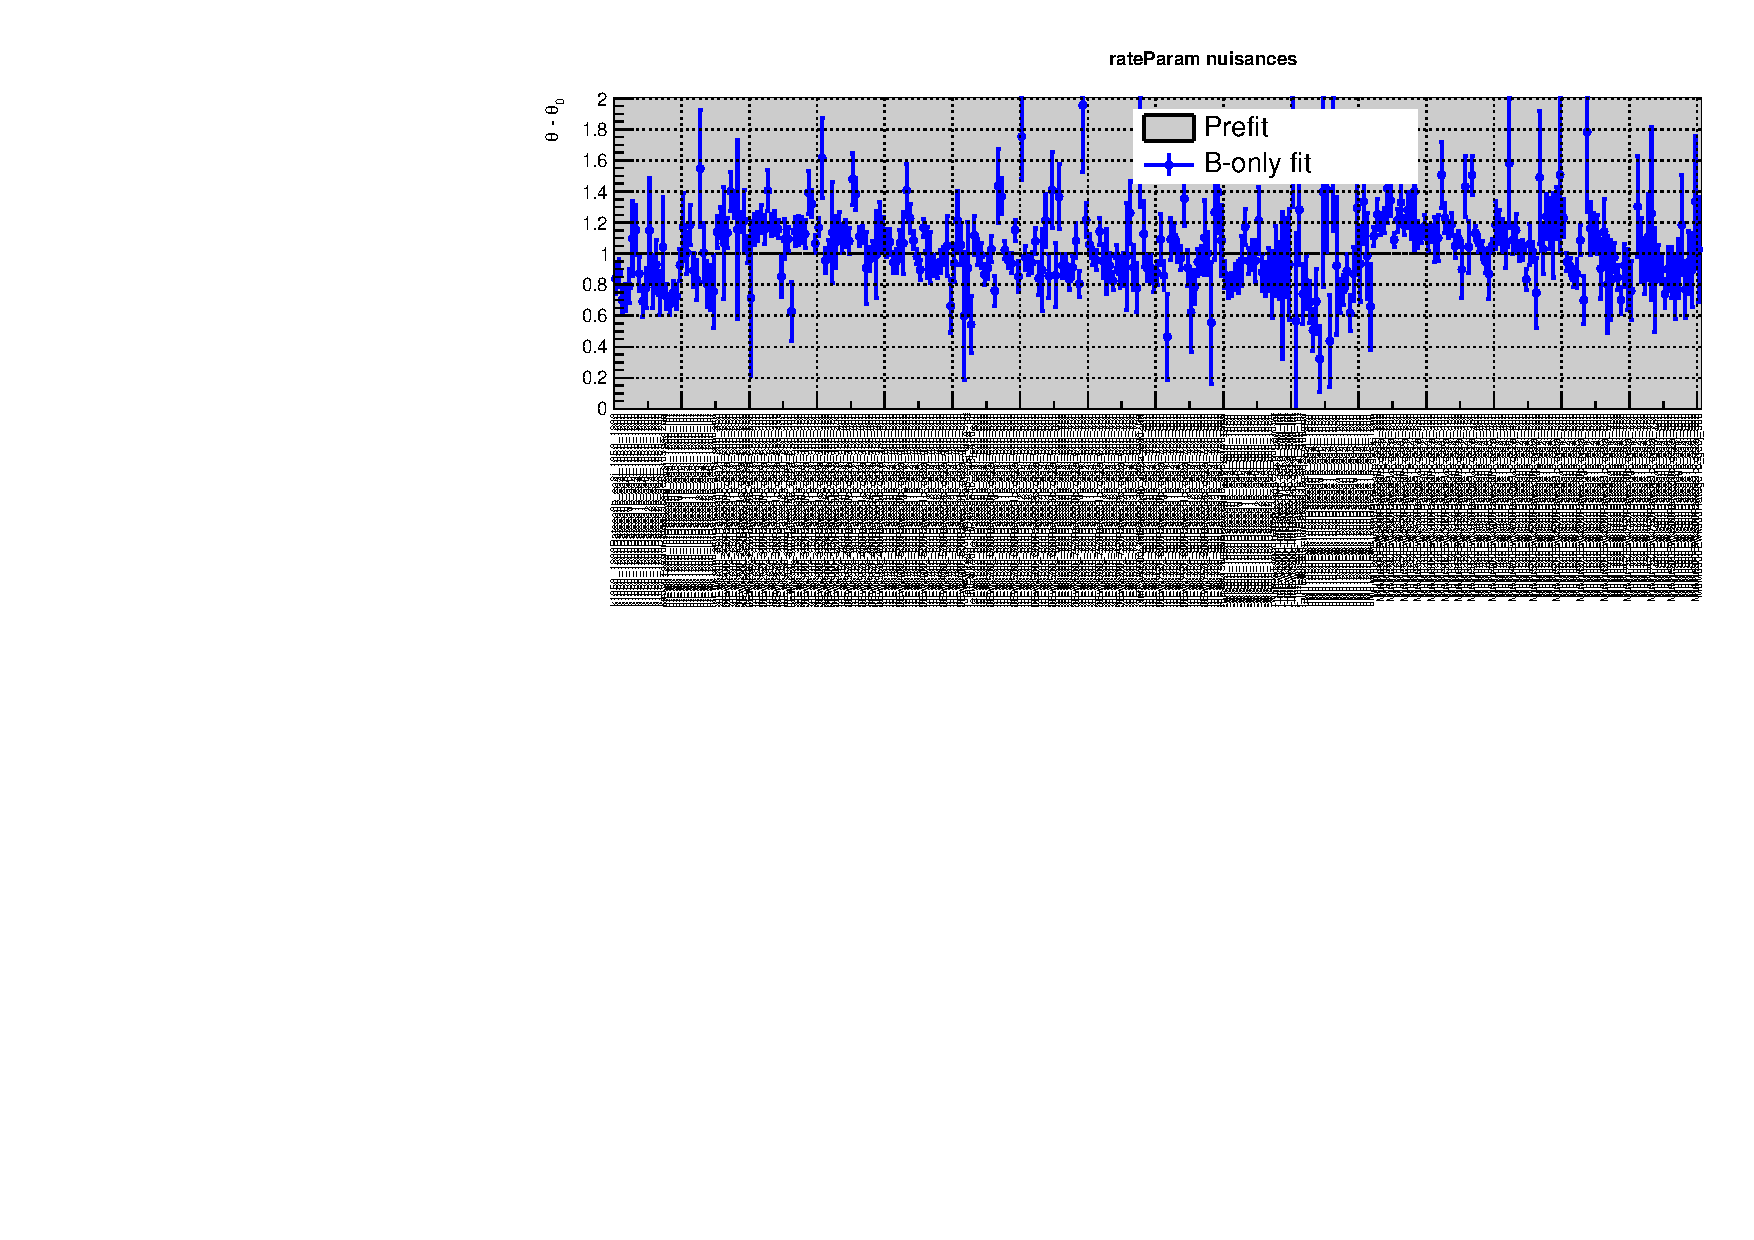
\includegraphics[width=1.\linewidth]{figures/results/36invfb/prefit/nuis/Rates_nuisances}
%\end{figure}
%
%\begin{figure}[h!]
%  \centering
%  \caption{Correlated sources of uncertainty}
%  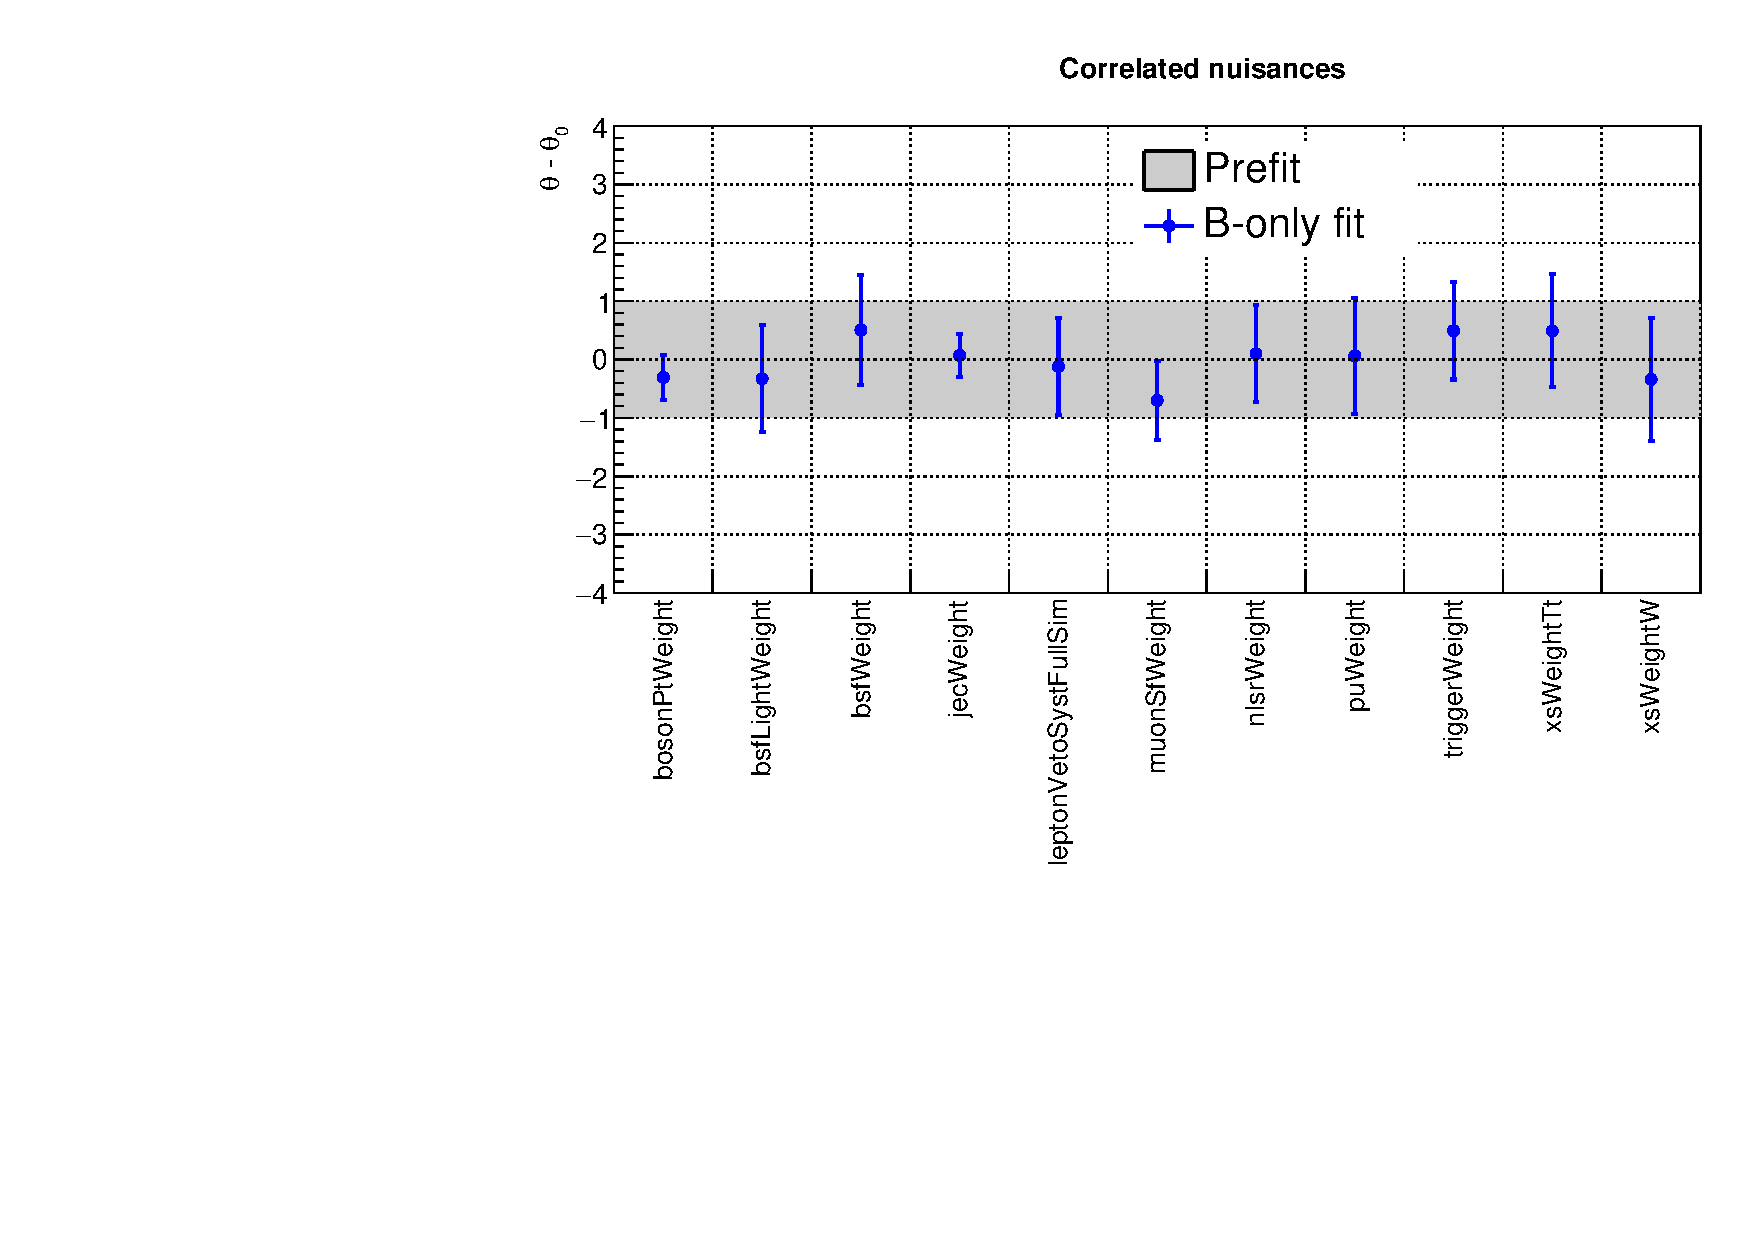
\includegraphics[width=1.\linewidth]{figures/results/36invfb/prefit/nuis/Correlated_nuisances}
%\end{figure}

\clearpage
\subsection{Post-fit nuisance parameters}
\label{app:nuispost}

\begin{figure}[h!]
  \centering
  \caption{Rate parameters}
  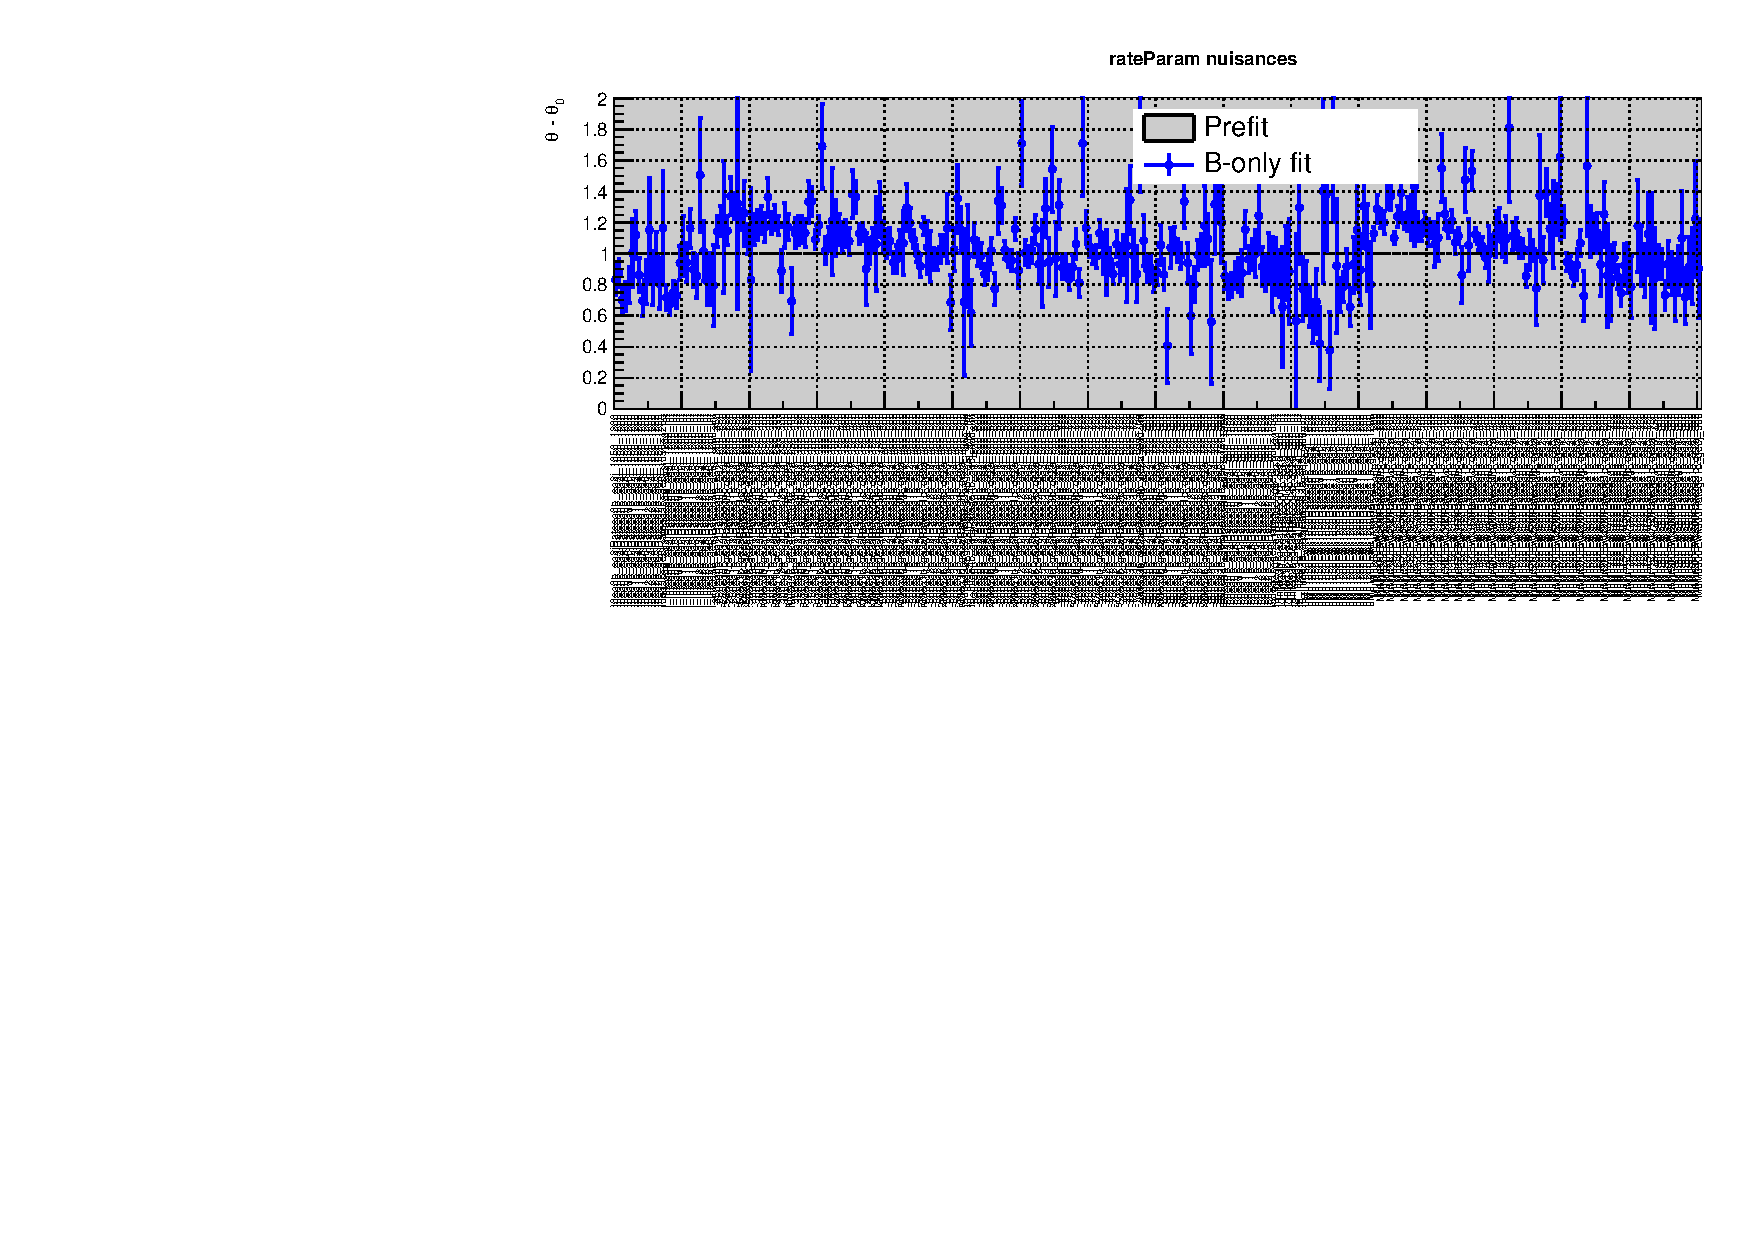
\includegraphics[width=1.\linewidth]{figures/results/36invfb_preapproval/postfit/nuis/Rates_nuisances}
\end{figure}

\begin{figure}[h!]
  \centering
  \caption{Correlated sources of uncertainty}
  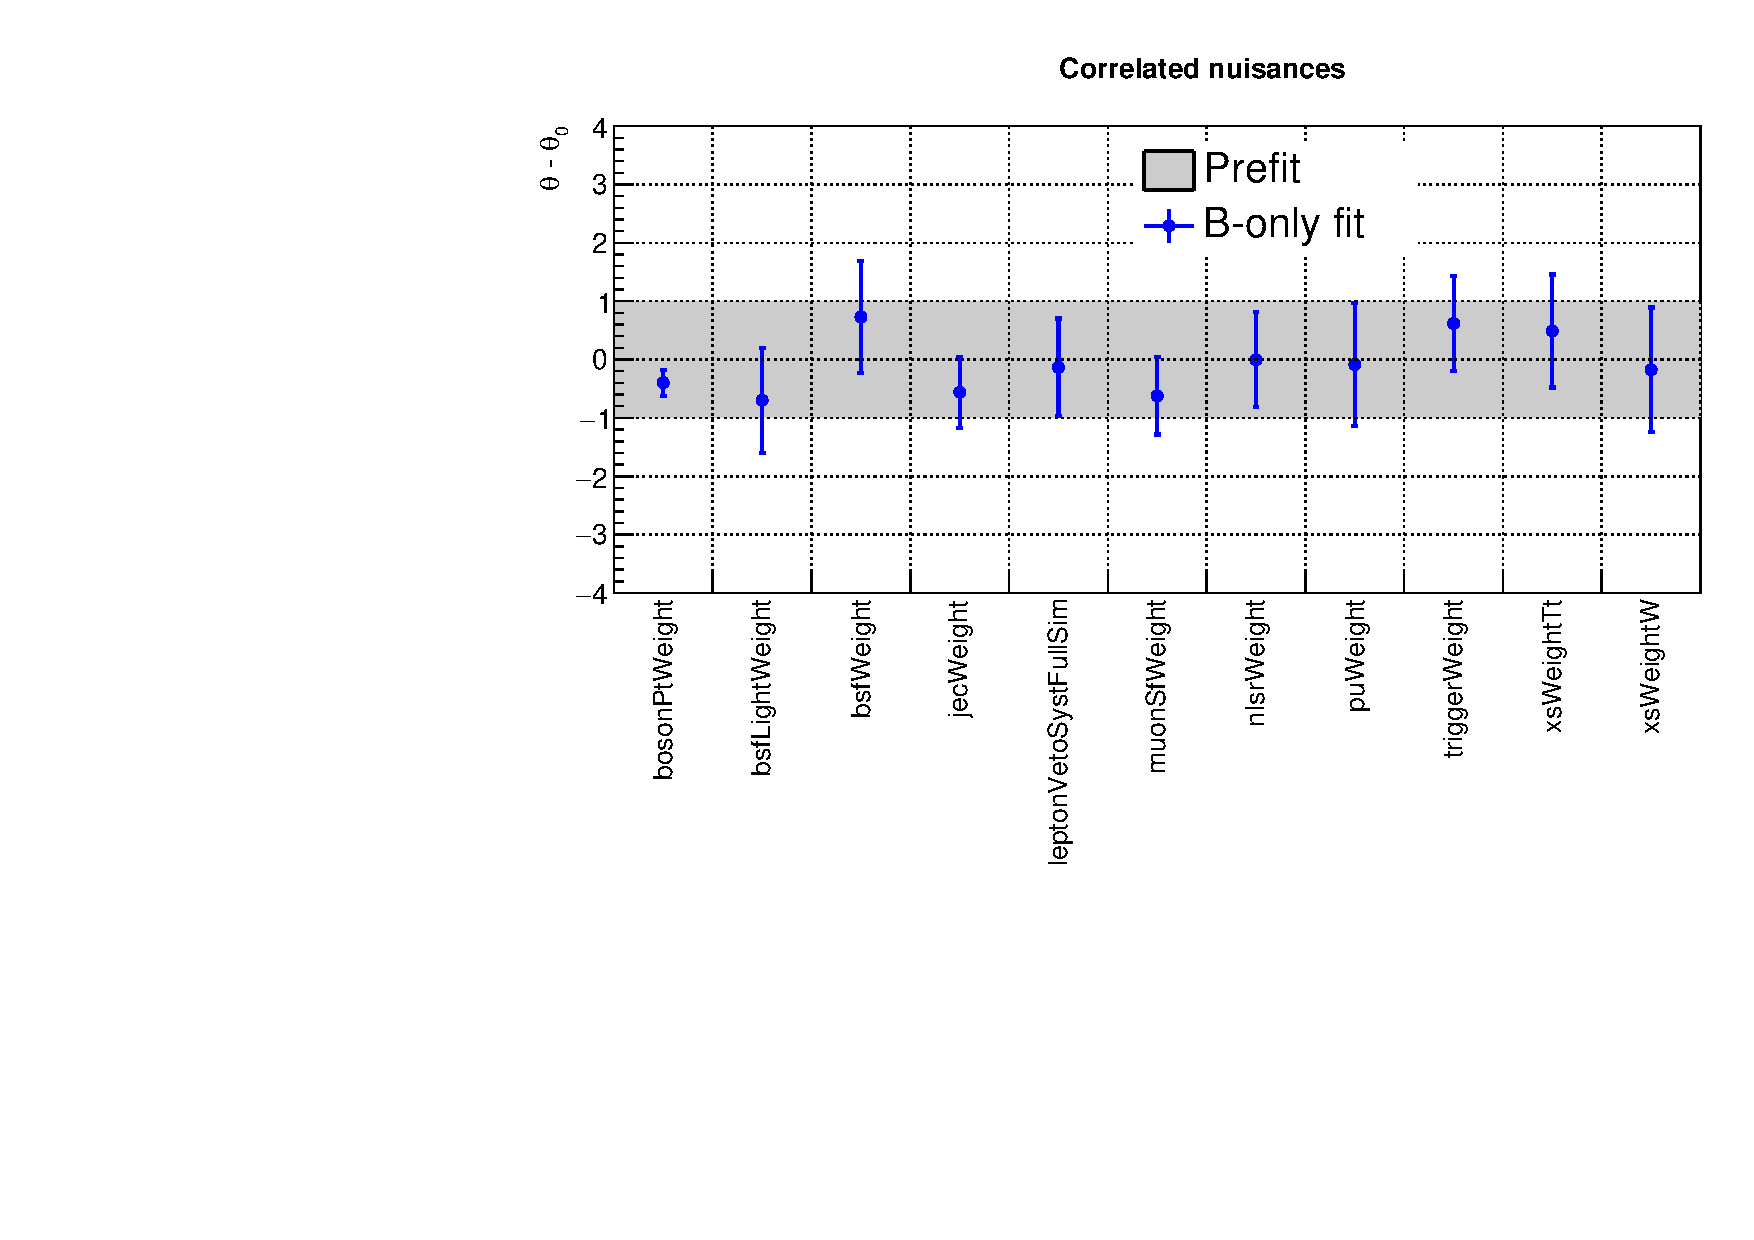
\includegraphics[width=1.\linewidth]{figures/results/36invfb_preapproval/postfit/nuis/Correlated_nuisances}
\end{figure}

\clearpage
\begin{figure}[h!]
  \centering
  \caption{``MC stat.'' uncertainties for lost lepton background.}
  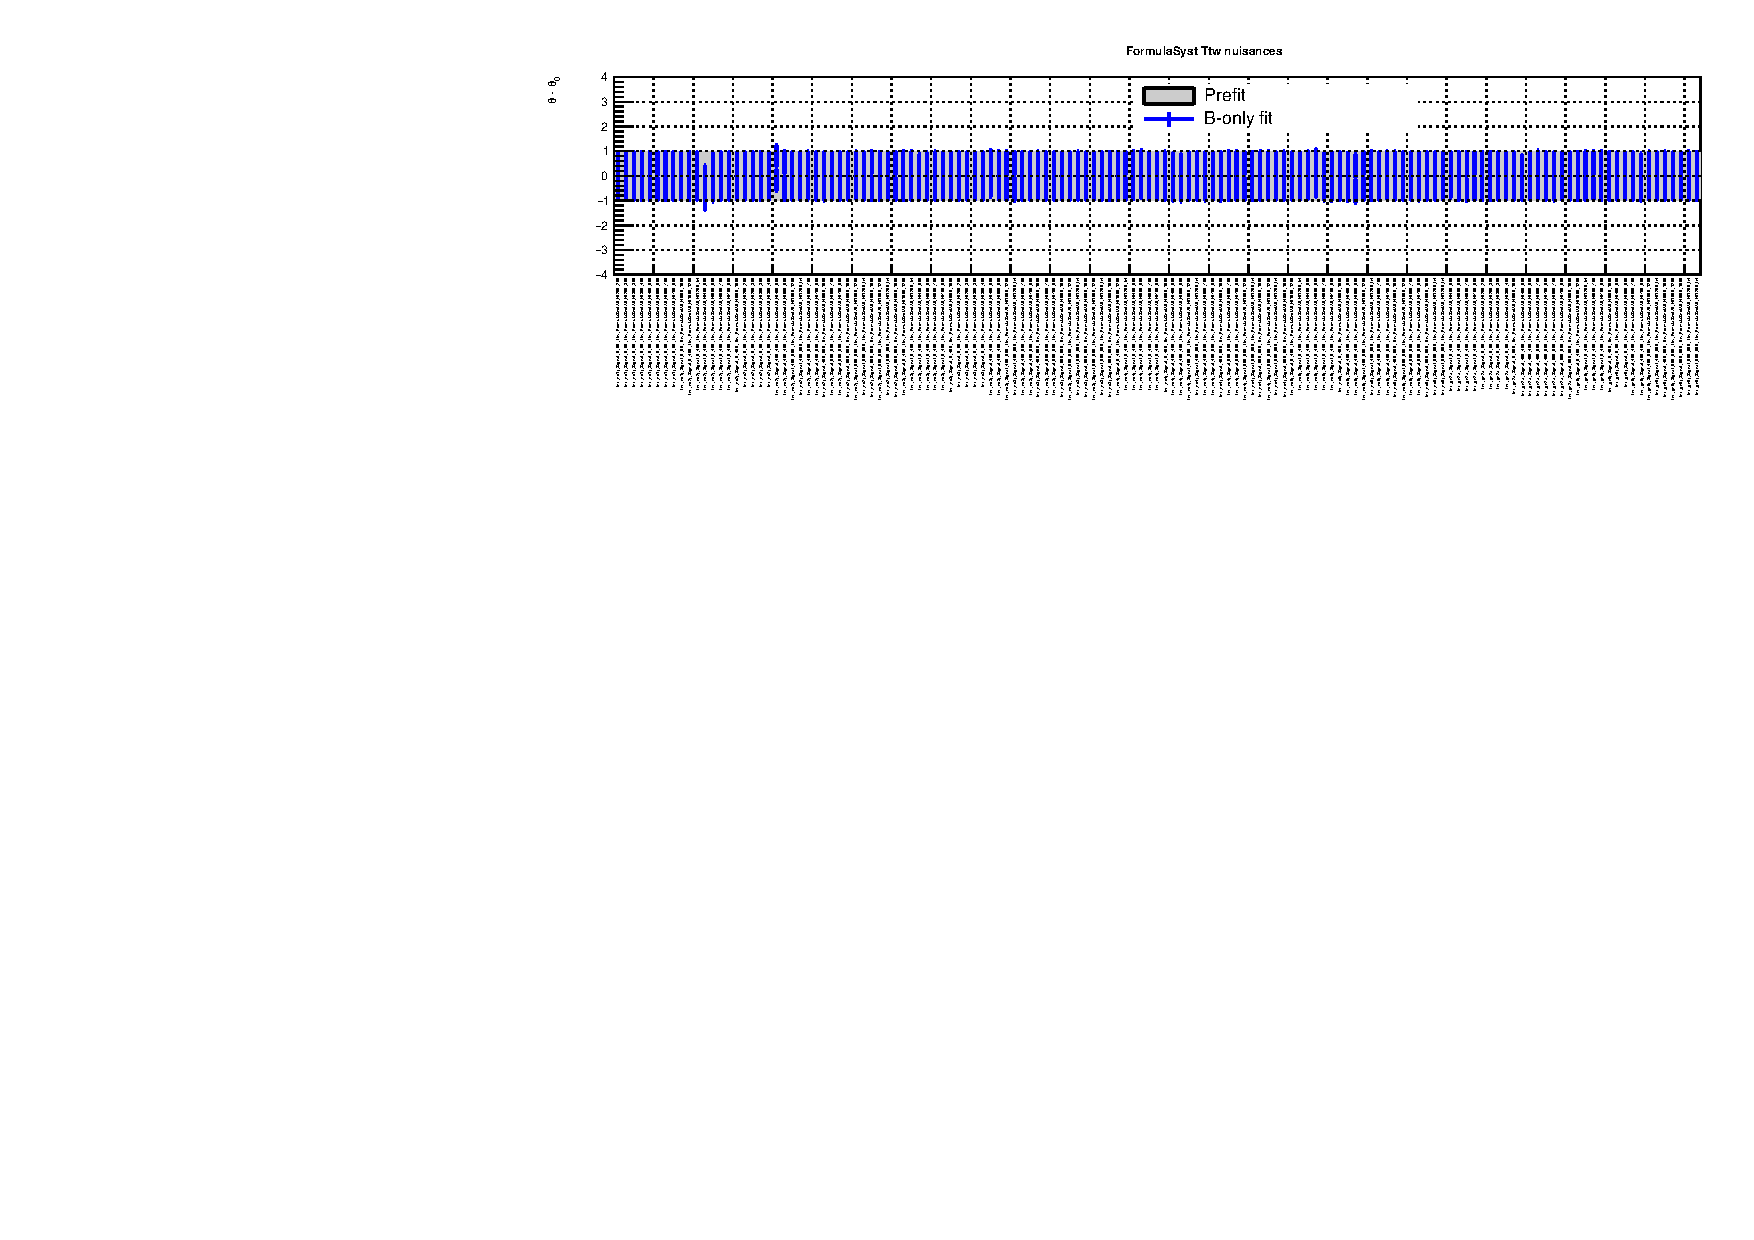
\includegraphics[width=1.\linewidth]{figures/results/36invfb_preapproval/postfit/nuis/FormulaSystTtw_nuisances}
\end{figure}

\begin{figure}[h!]
  \centering
  \caption{``MC stat.'' uncertainties for \znunuj background.}
  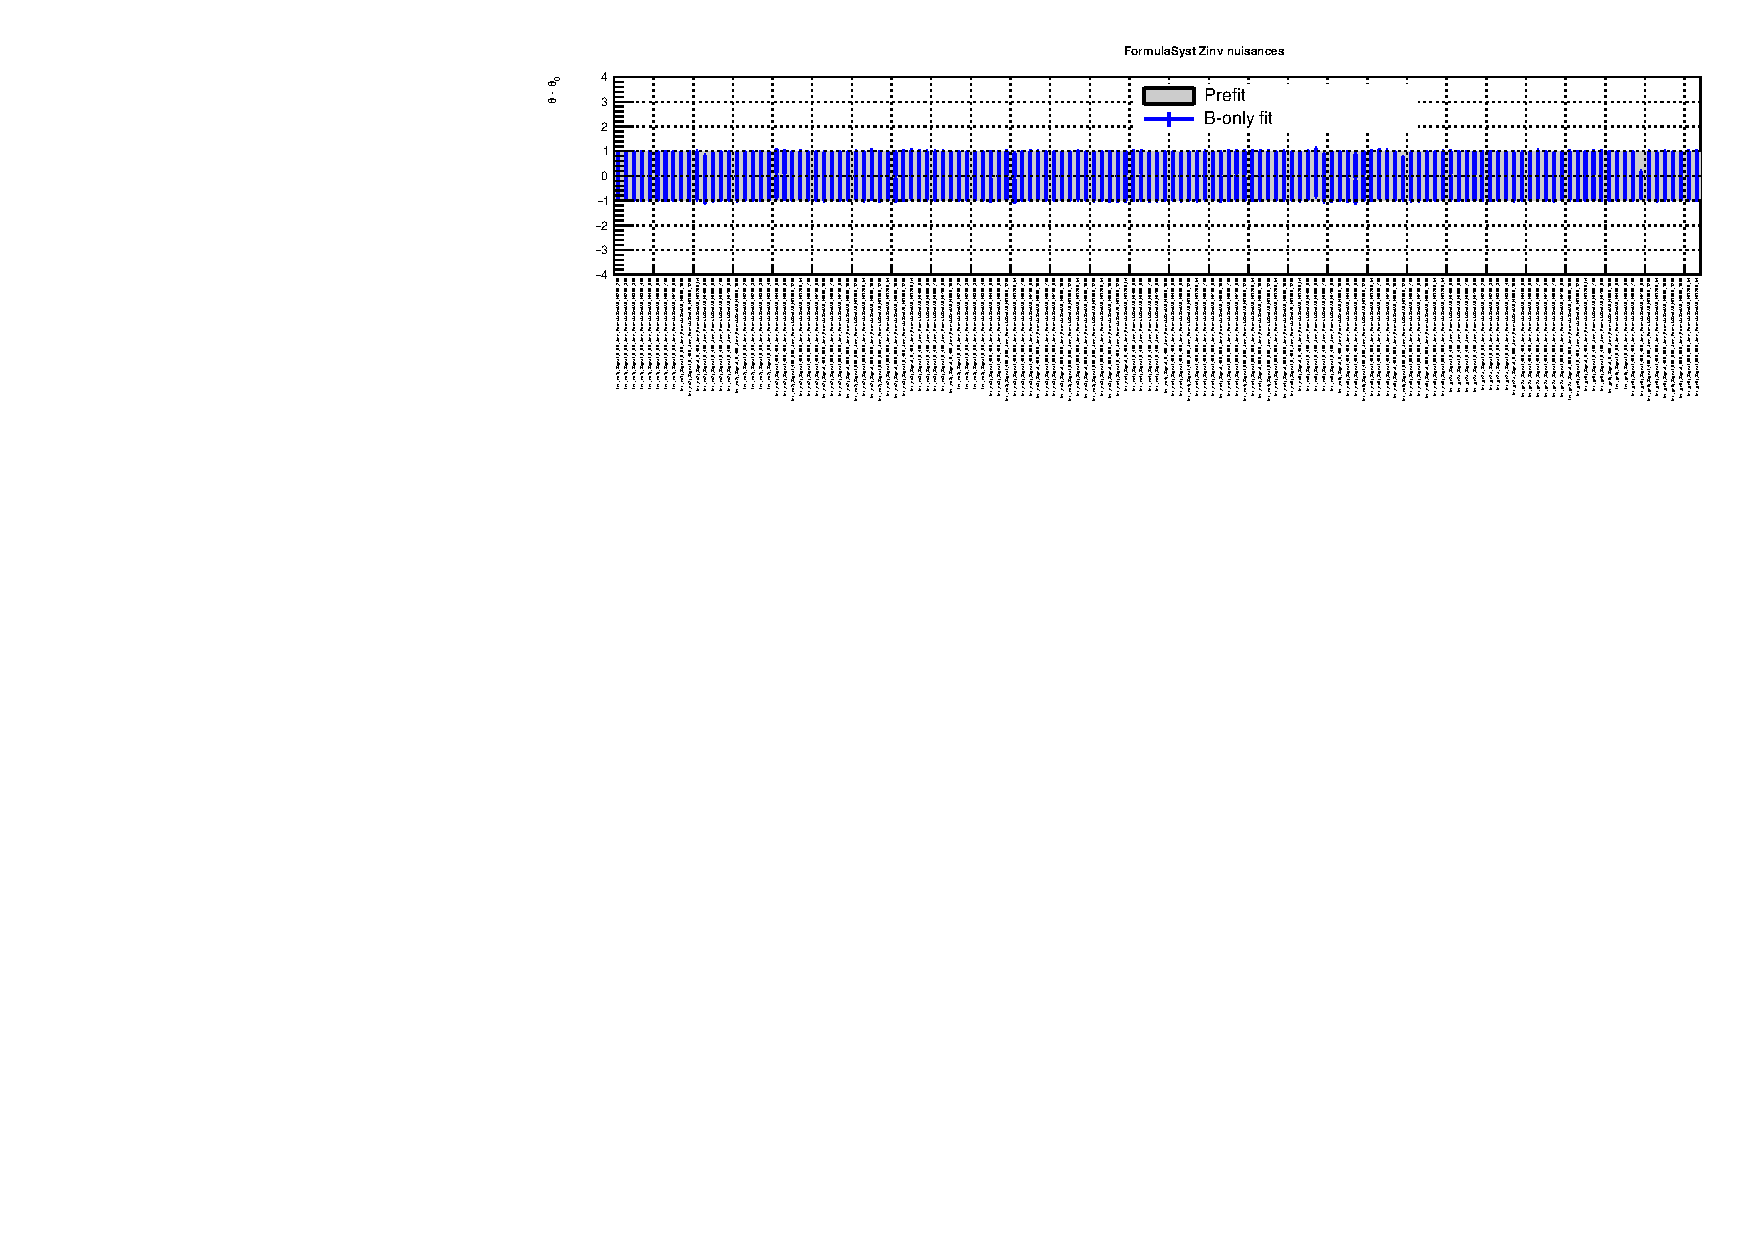
\includegraphics[width=1.\linewidth]{figures/results/36invfb_preapproval/postfit/nuis/FormulaSystZinv_nuisances}
\end{figure}

\clearpage
\begin{figure}[h!]
  \centering
  \caption{Systematic uncertainties in QCD background estimate}
  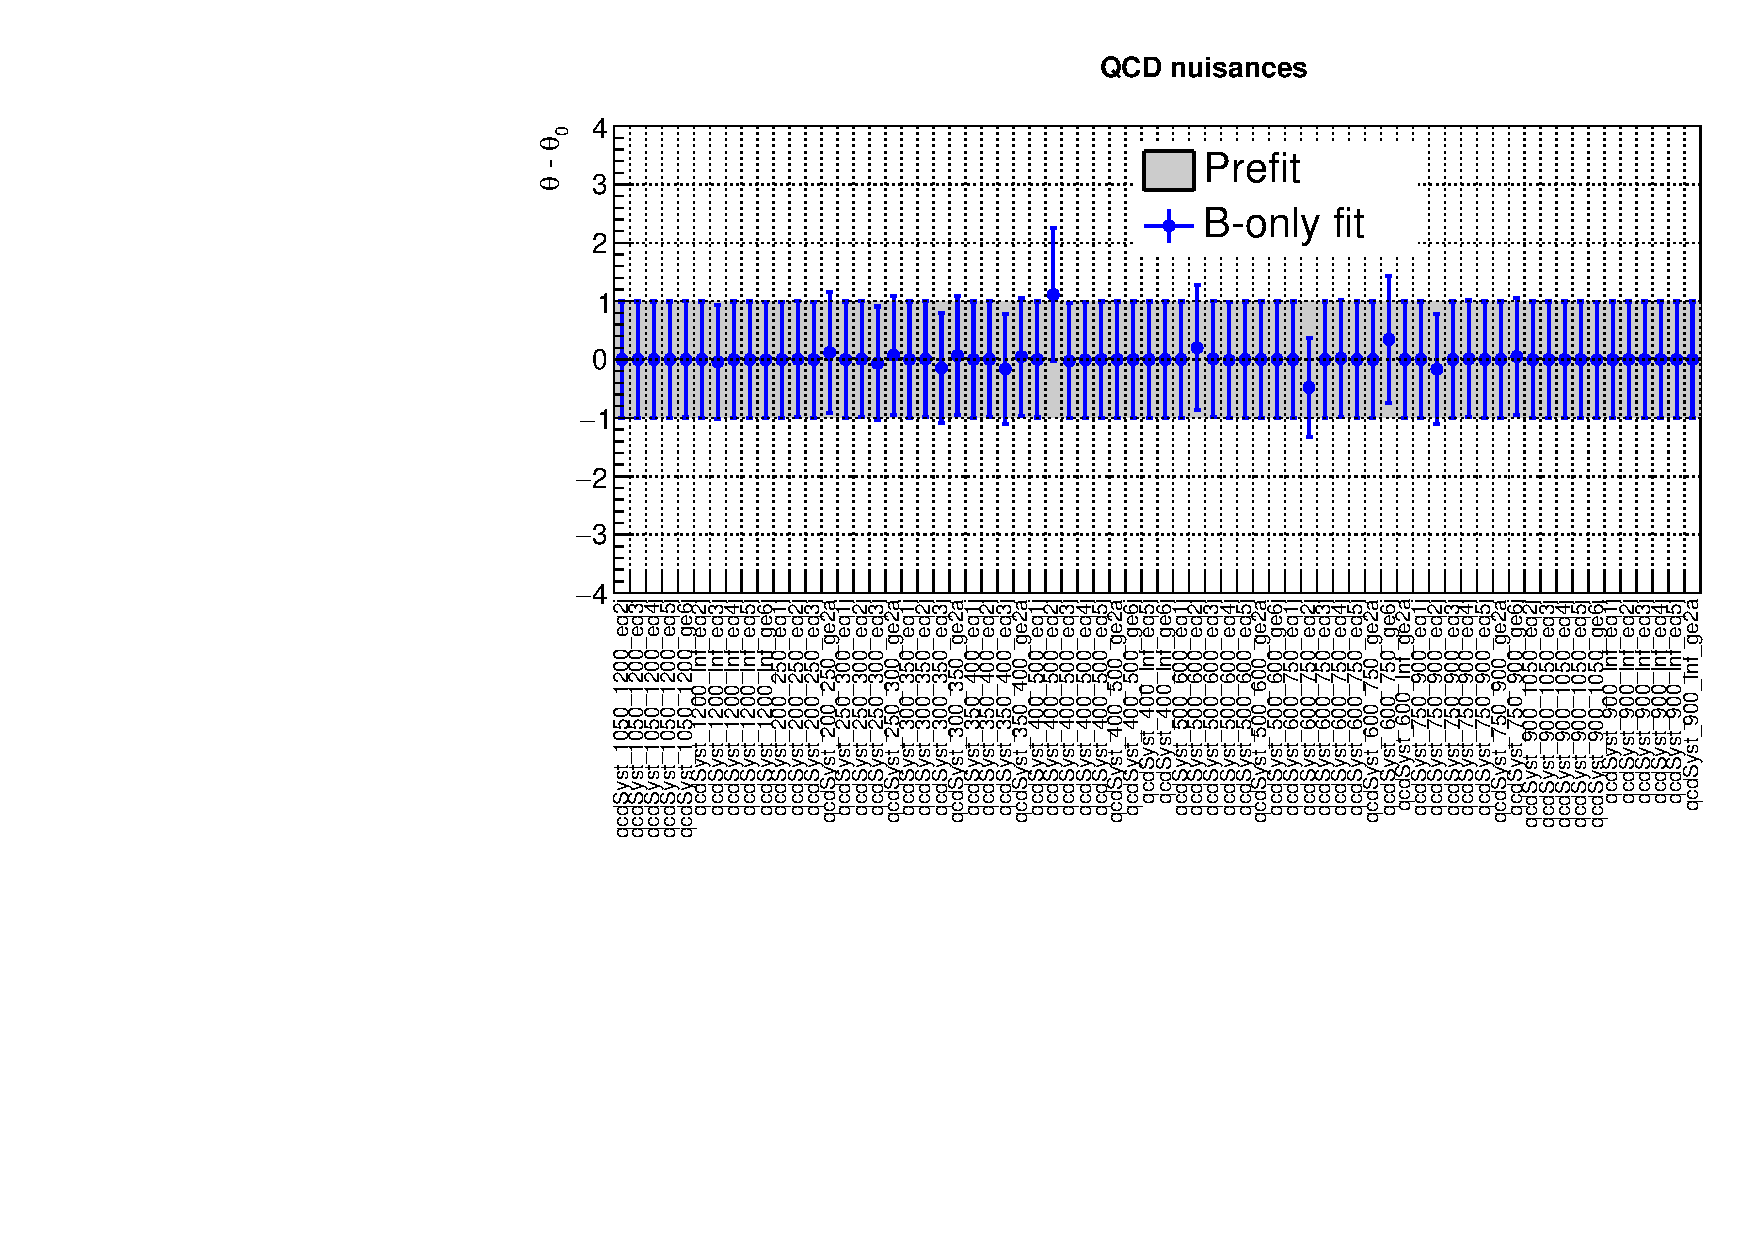
\includegraphics[width=1.\linewidth]{figures/results/36invfb_preapproval/postfit/nuis/qcd_nuisances}
\end{figure}

\clearpage
\begin{figure}[h!]
  \centering
  \caption{Systematic uncertainties per \scalht category in \mht modelling for lost lepton background}
  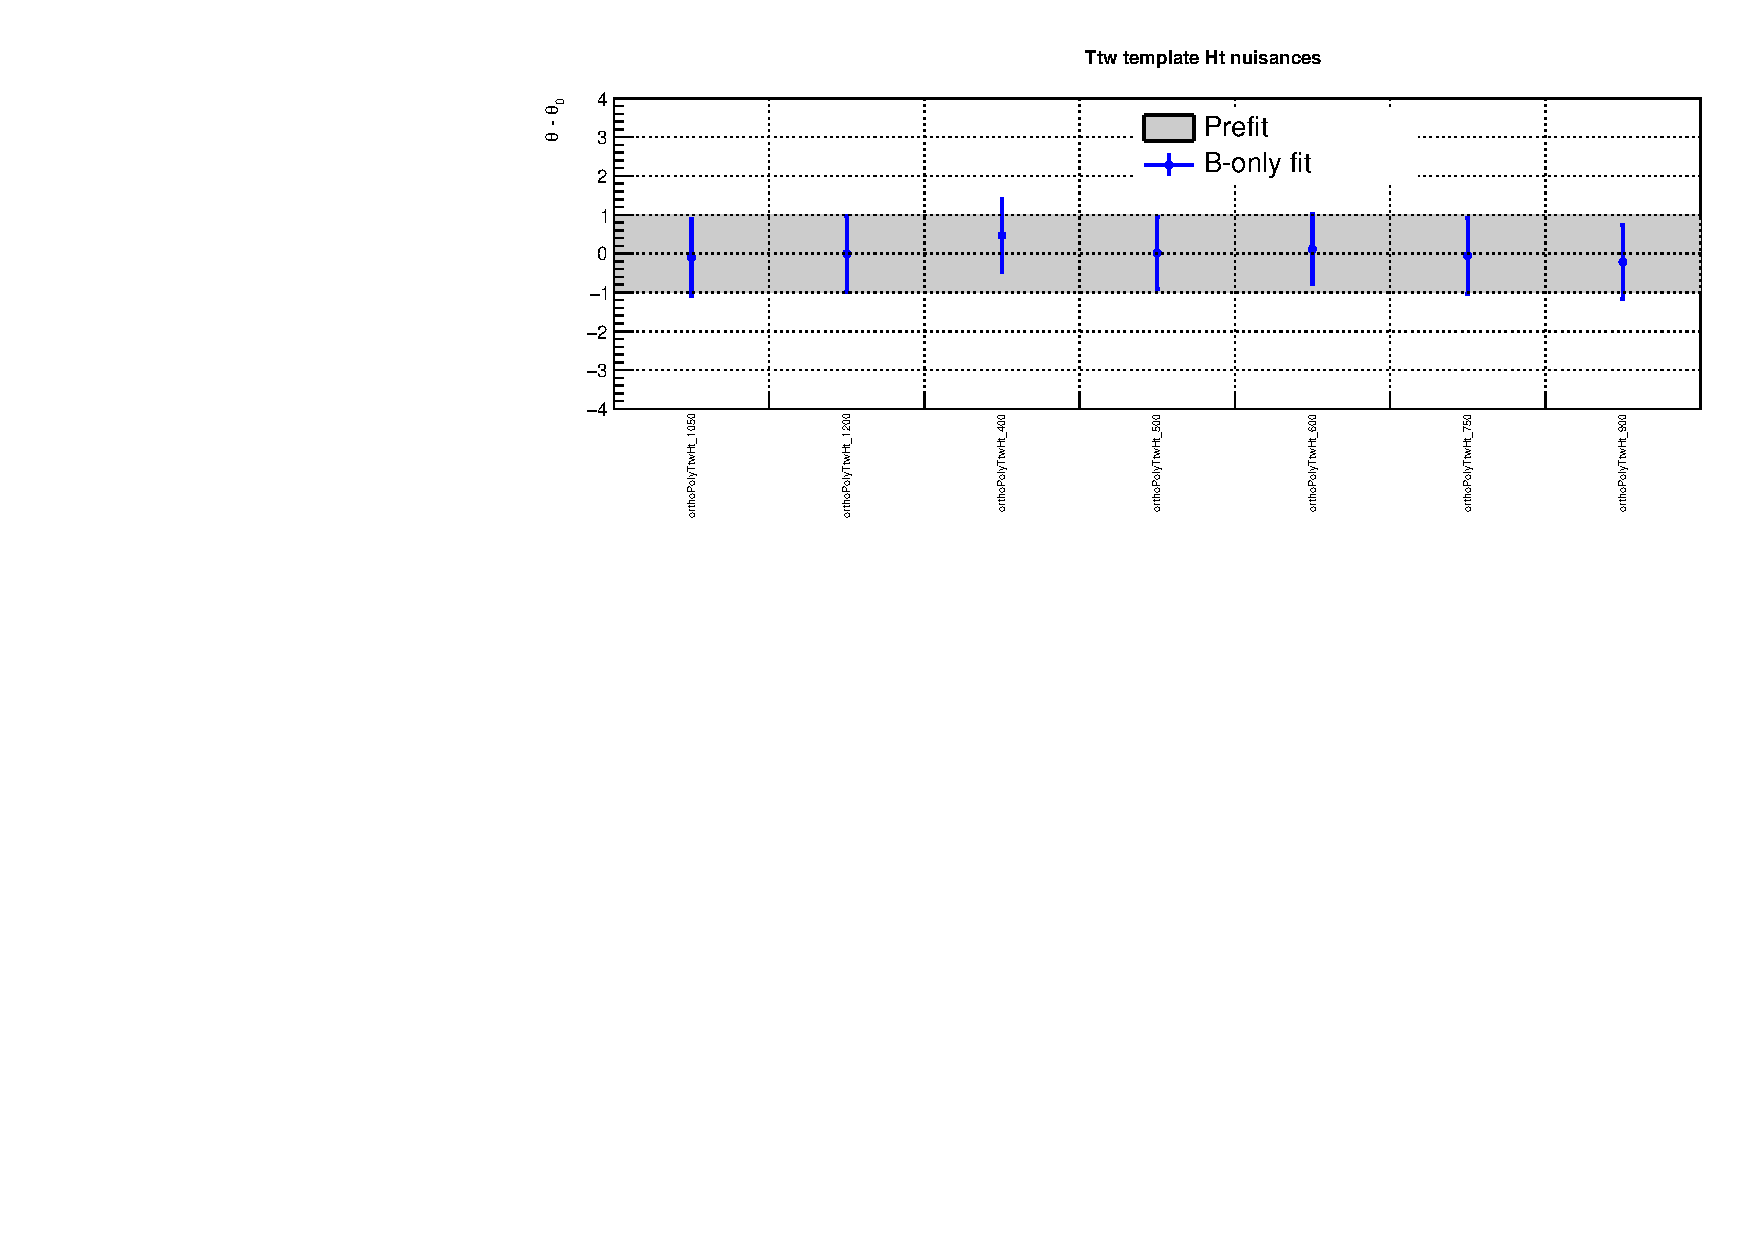
\includegraphics[width=1.\linewidth]{figures/results/36invfb_preapproval/postfit/nuis/TemplateTtw_ht_nuisances}
\end{figure}

\begin{figure}[h!]
  \centering
  \caption{Systematic uncertainties per \njet category in \mht modelling for lost lepton background}
  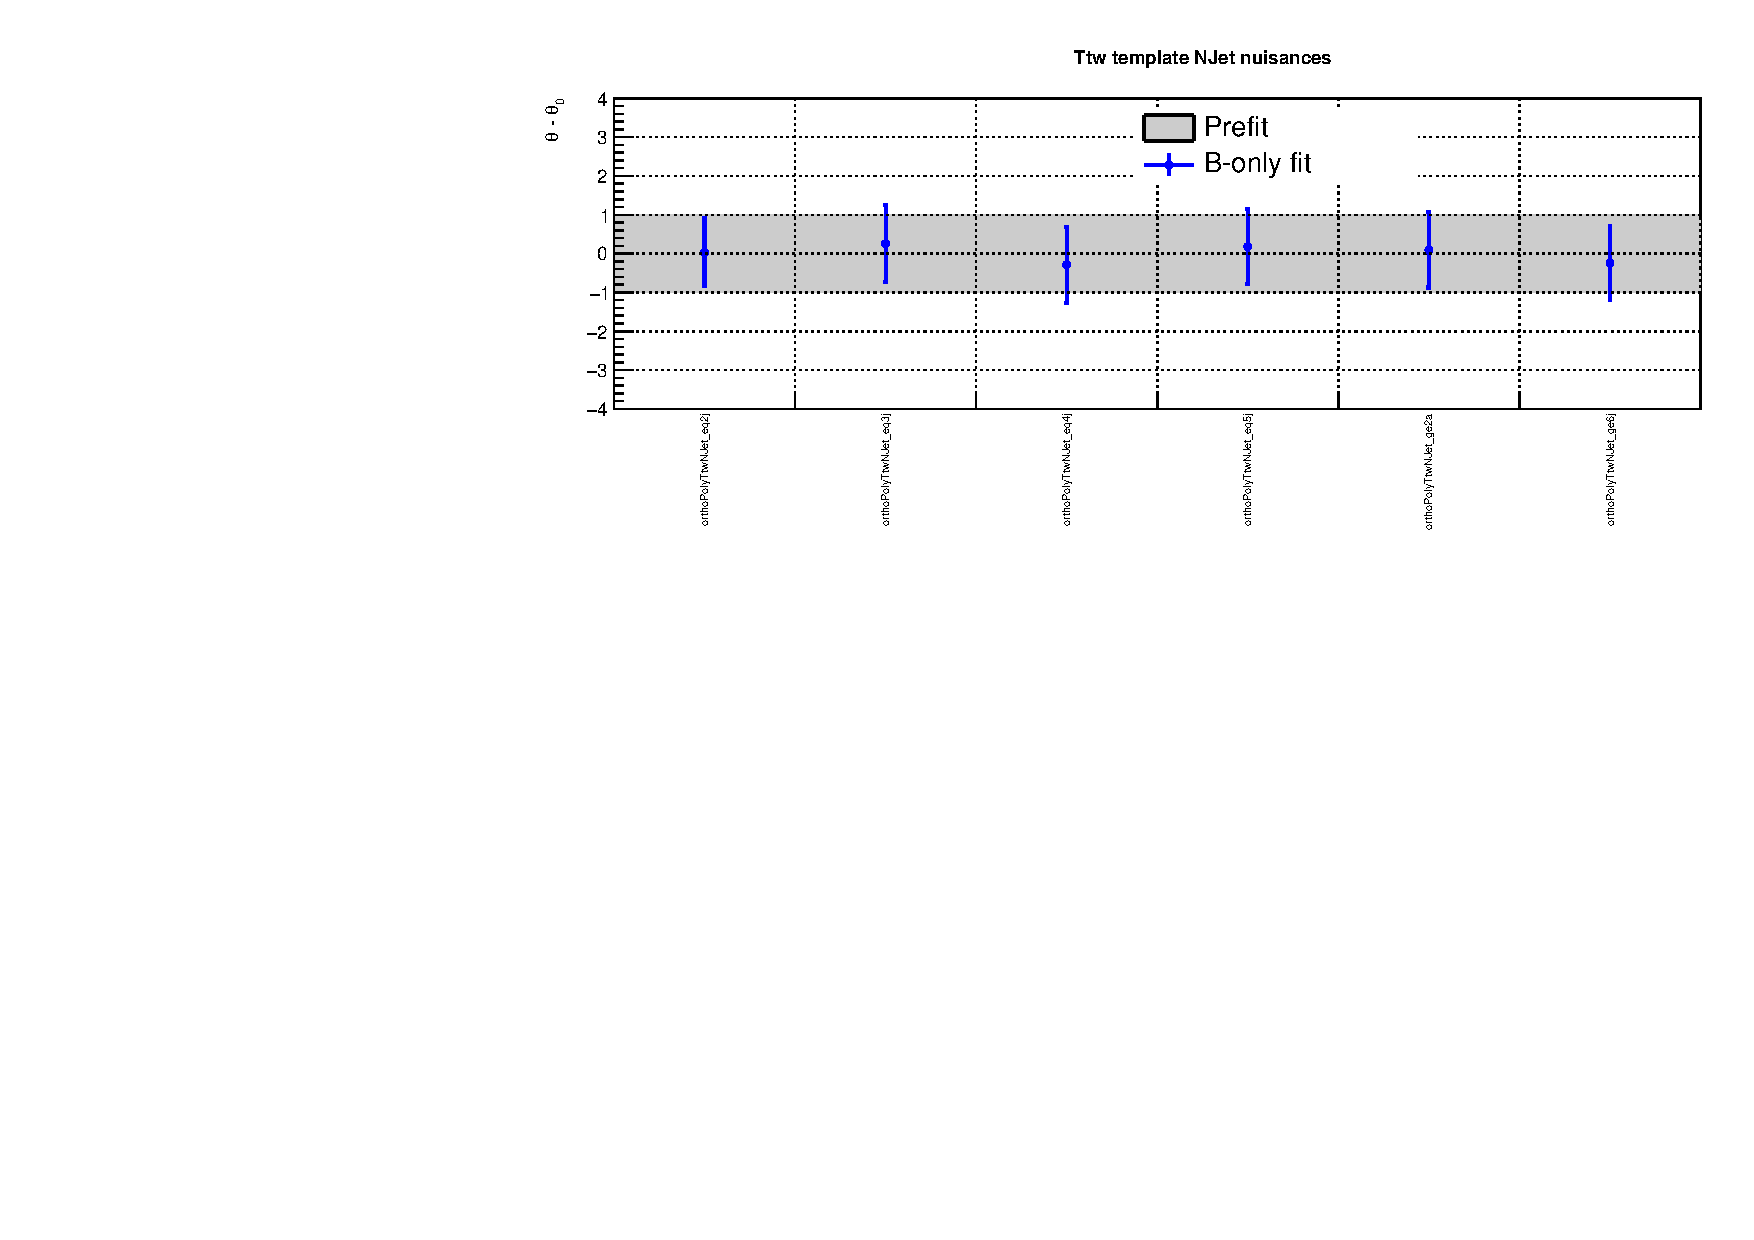
\includegraphics[width=1.\linewidth]{figures/results/36invfb_preapproval/postfit/nuis/TemplateTtw_njet_nuisances}
\end{figure}

\clearpage
\begin{figure}[h!]
  \centering
  \caption{Systematic uncertainties per \scalht category in \mht modelling for \znunuj background}
  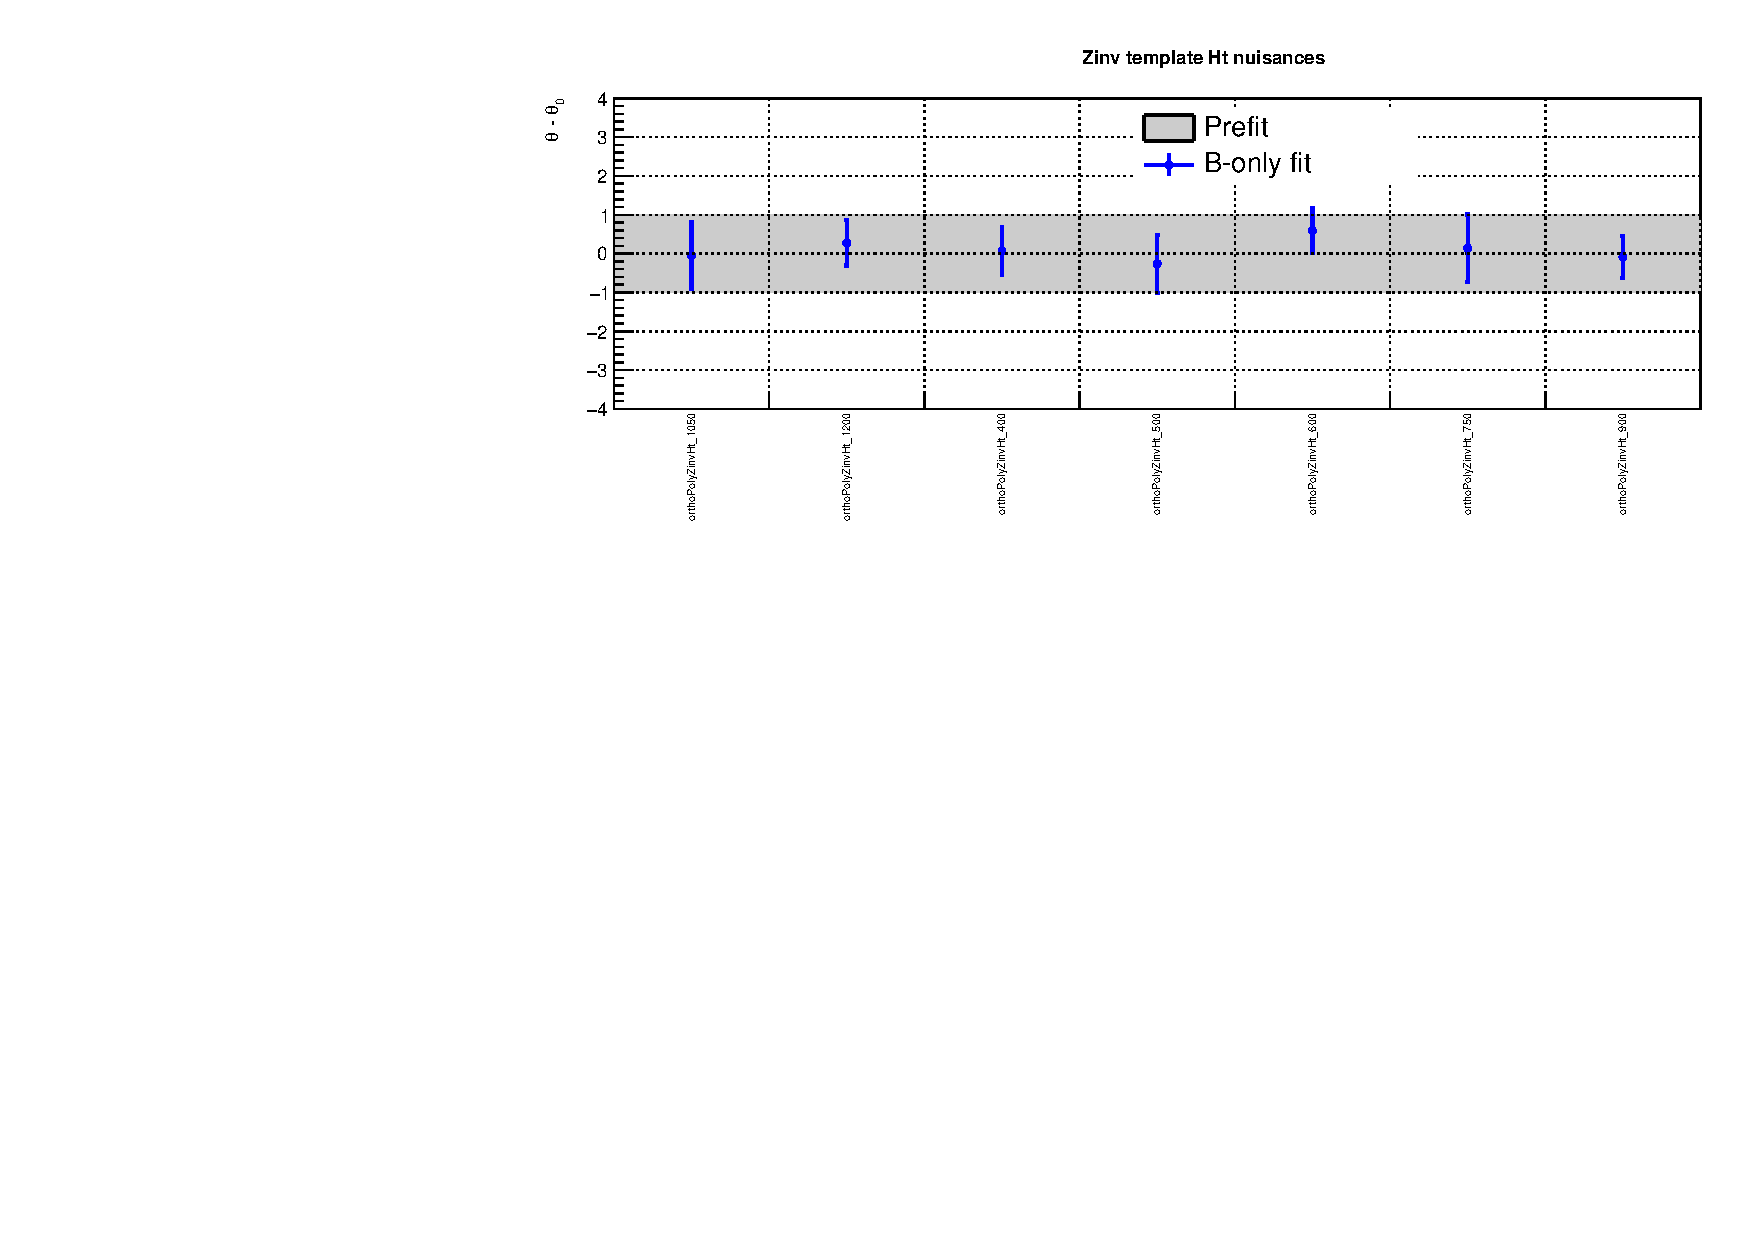
\includegraphics[width=1.\linewidth]{figures/results/36invfb_preapproval/postfit/nuis/TemplateZinv_ht_nuisances}
\end{figure}

\begin{figure}[h!]
  \centering
  \caption{Systematic uncertainties per \njet category in \mht modelling for \znunuj background}
  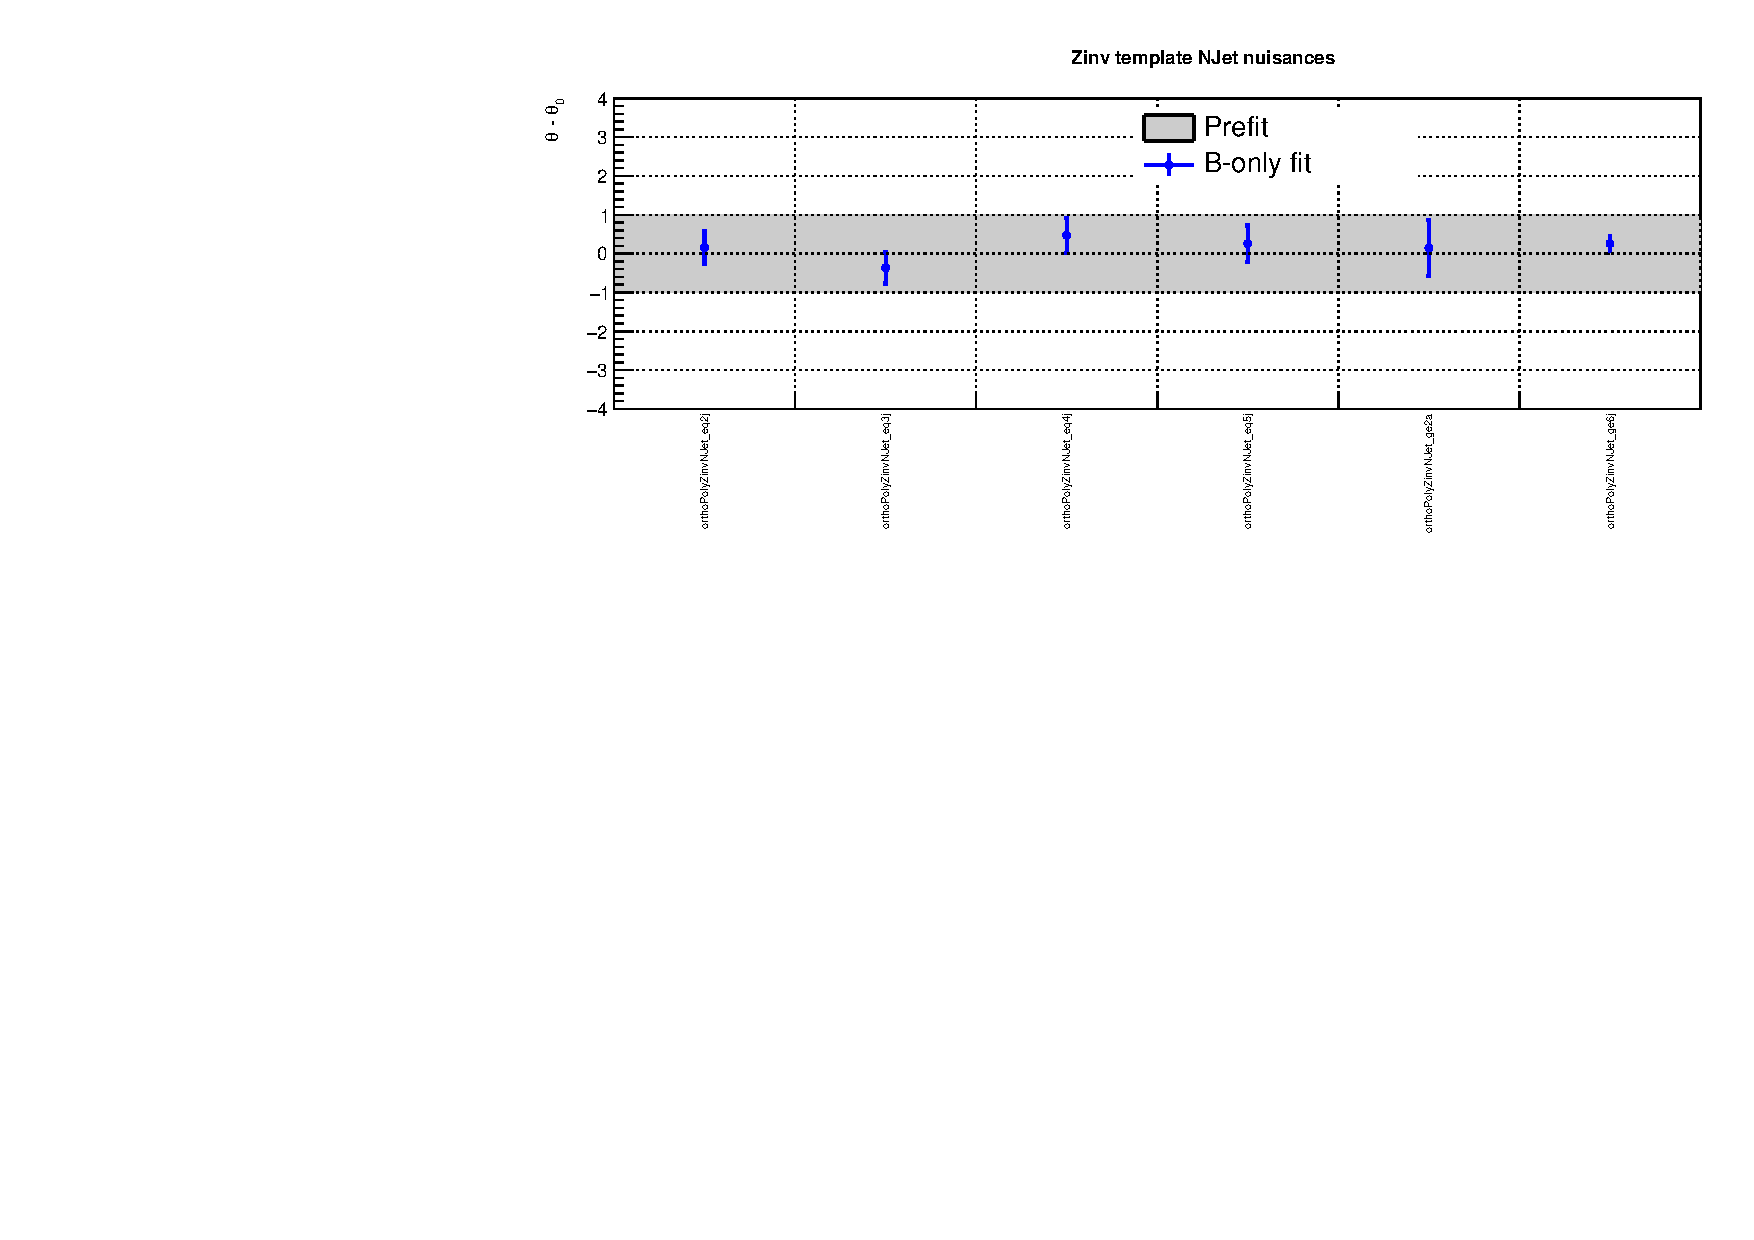
\includegraphics[width=1.\linewidth]{figures/results/36invfb_preapproval/postfit/nuis/TemplateZinv_njet_nuisances}
\end{figure}

\clearpage
\begin{figure}[h!]
  \centering
  \caption{Systematic uncertainties in \alphat modelling}
  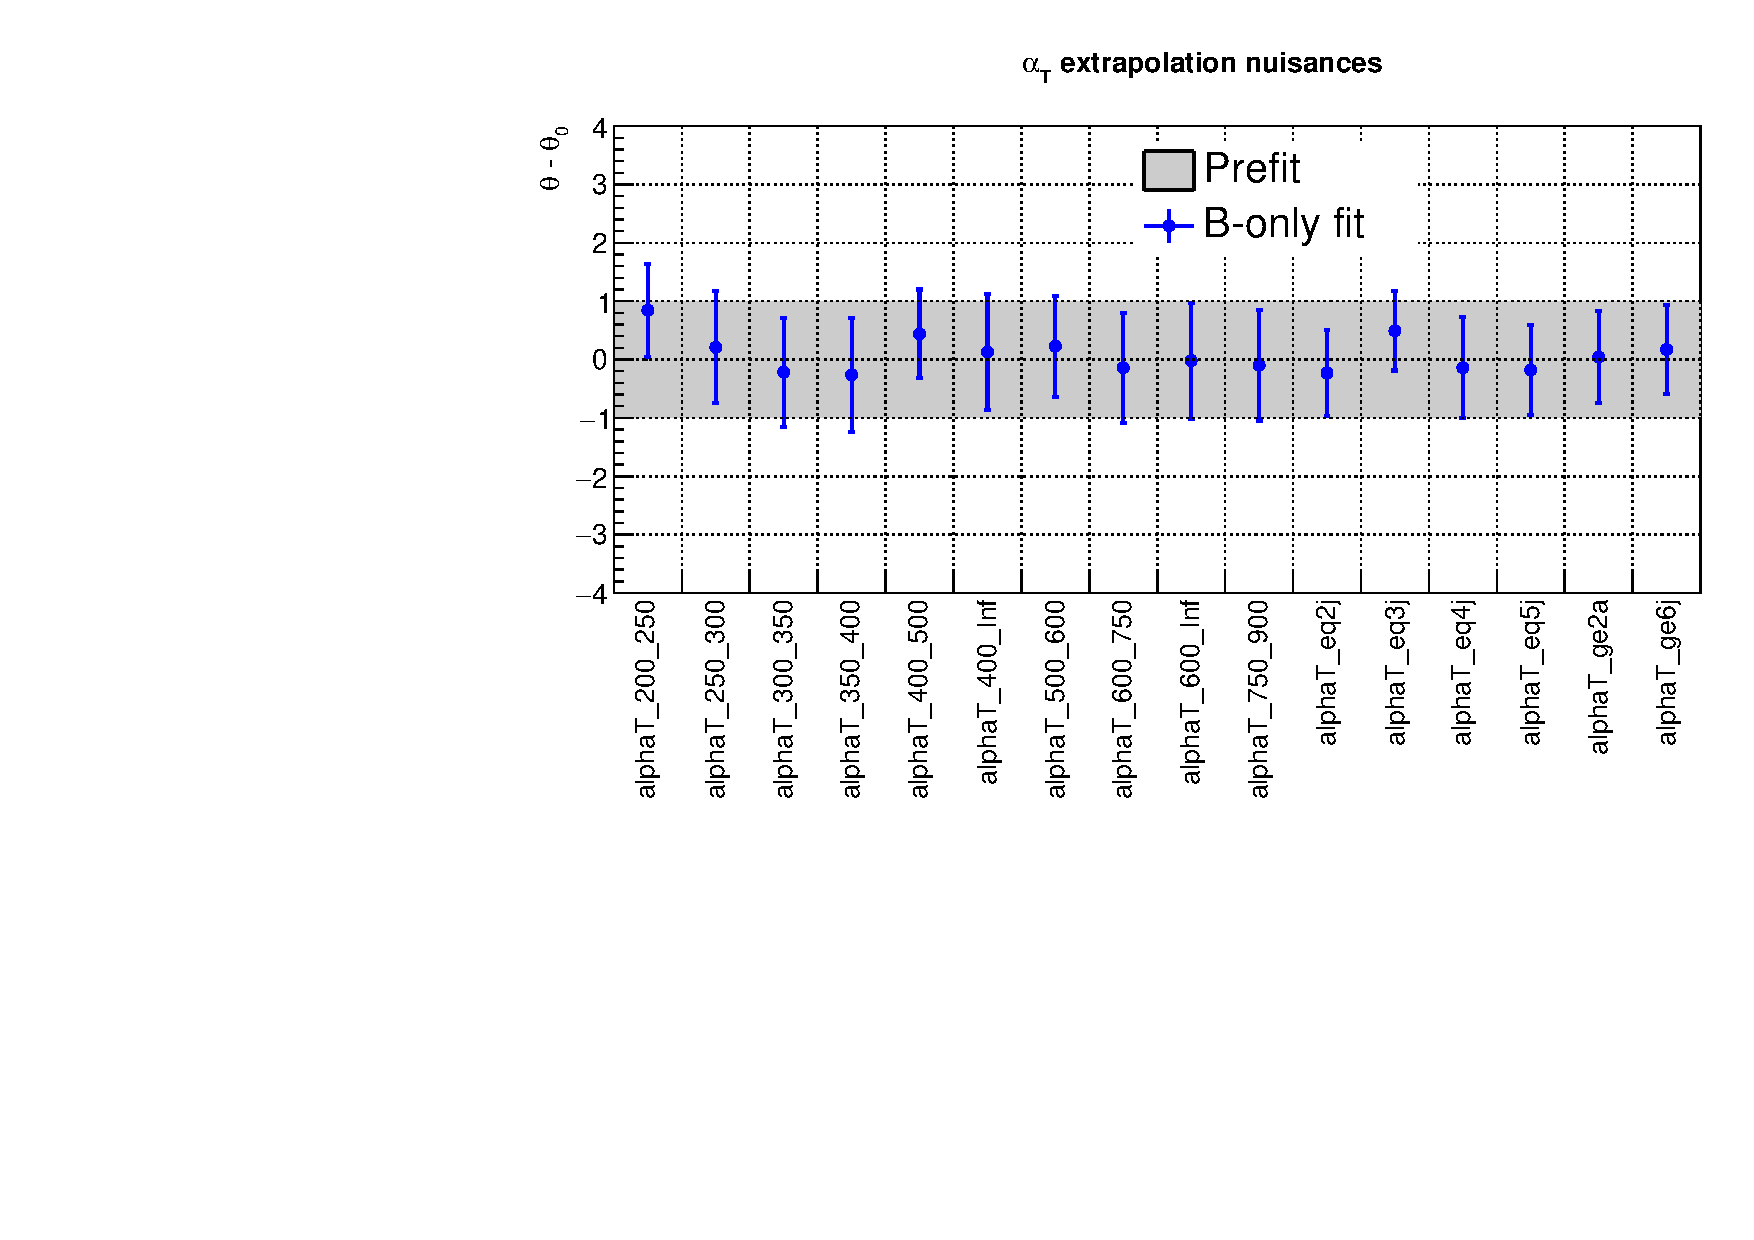
\includegraphics[width=0.8\linewidth]{figures/results/36invfb_preapproval/postfit/nuis/AlphaT_nuisances}
\end{figure}

\begin{figure}[h!]
  \centering
  \caption{Systematic uncertainties in \bdphi modelling}
  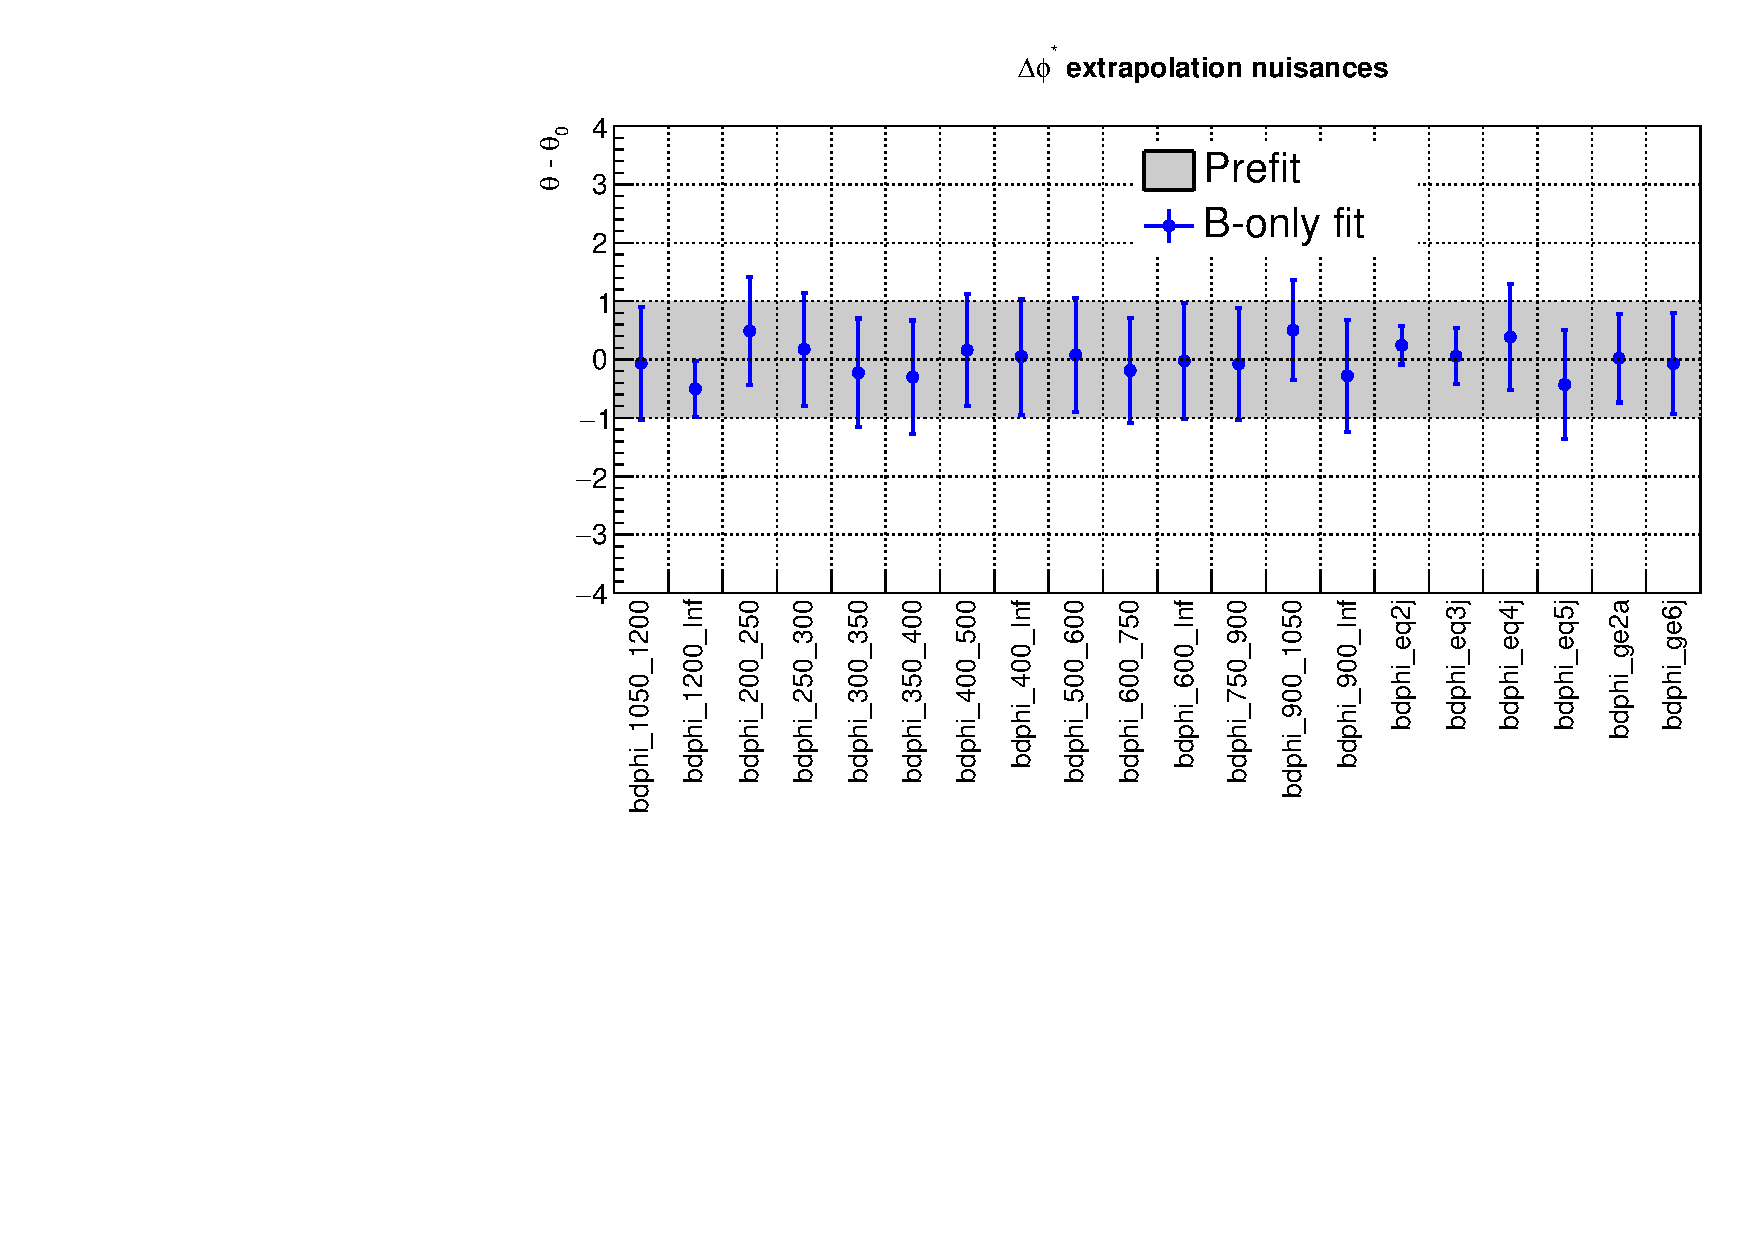
\includegraphics[width=0.8\linewidth]{figures/results/36invfb_preapproval/postfit/nuis/bDPhi_nuisances}
\end{figure}

\clearpage
\begin{figure}[h!]
  \centering
  \caption{Systematic uncertainties in single isolated track veto modelling}
  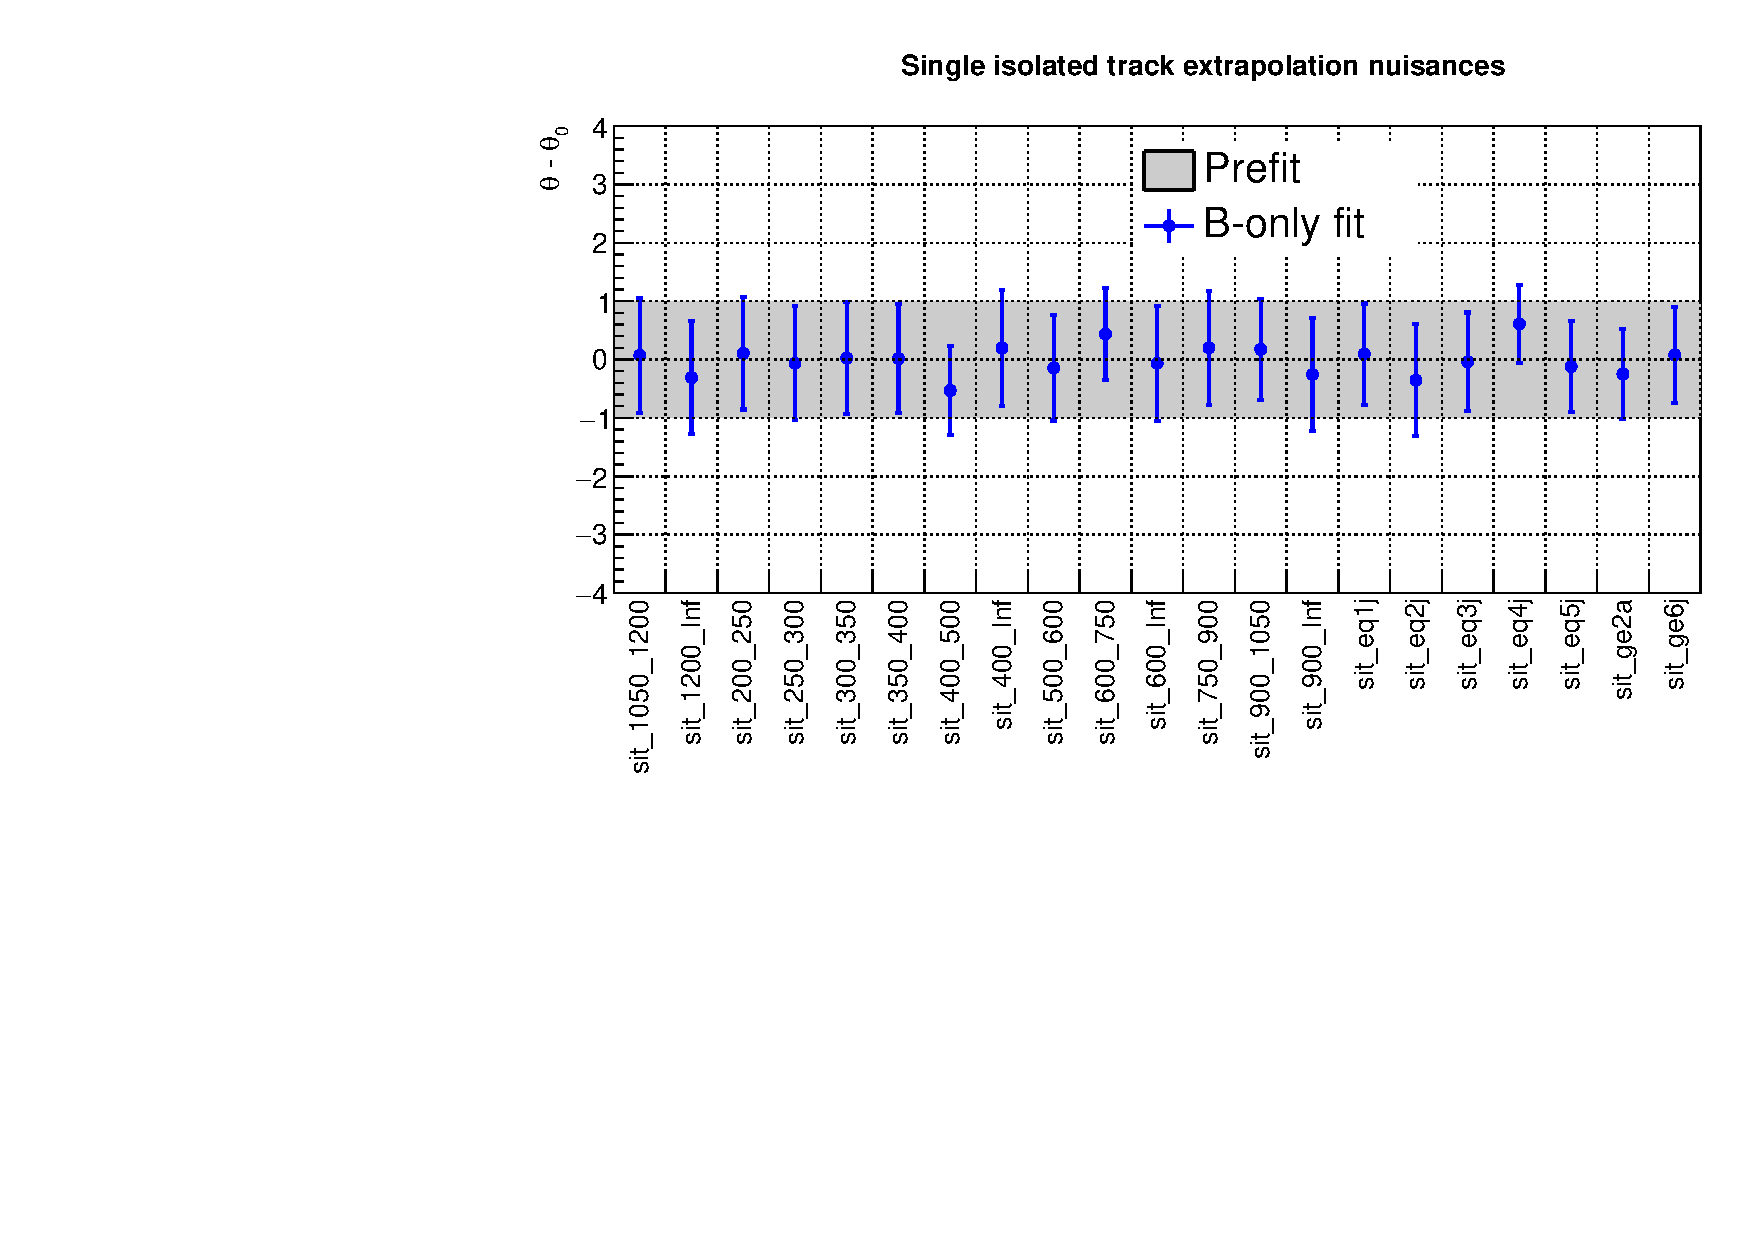
\includegraphics[width=0.8\linewidth]{figures/results/36invfb_preapproval/postfit/nuis/SIT_nuisances}
\end{figure}

\clearpage
\begin{figure}[h!]
  \centering
  \caption{Systematic uncertainties in W polarisation modelling}
  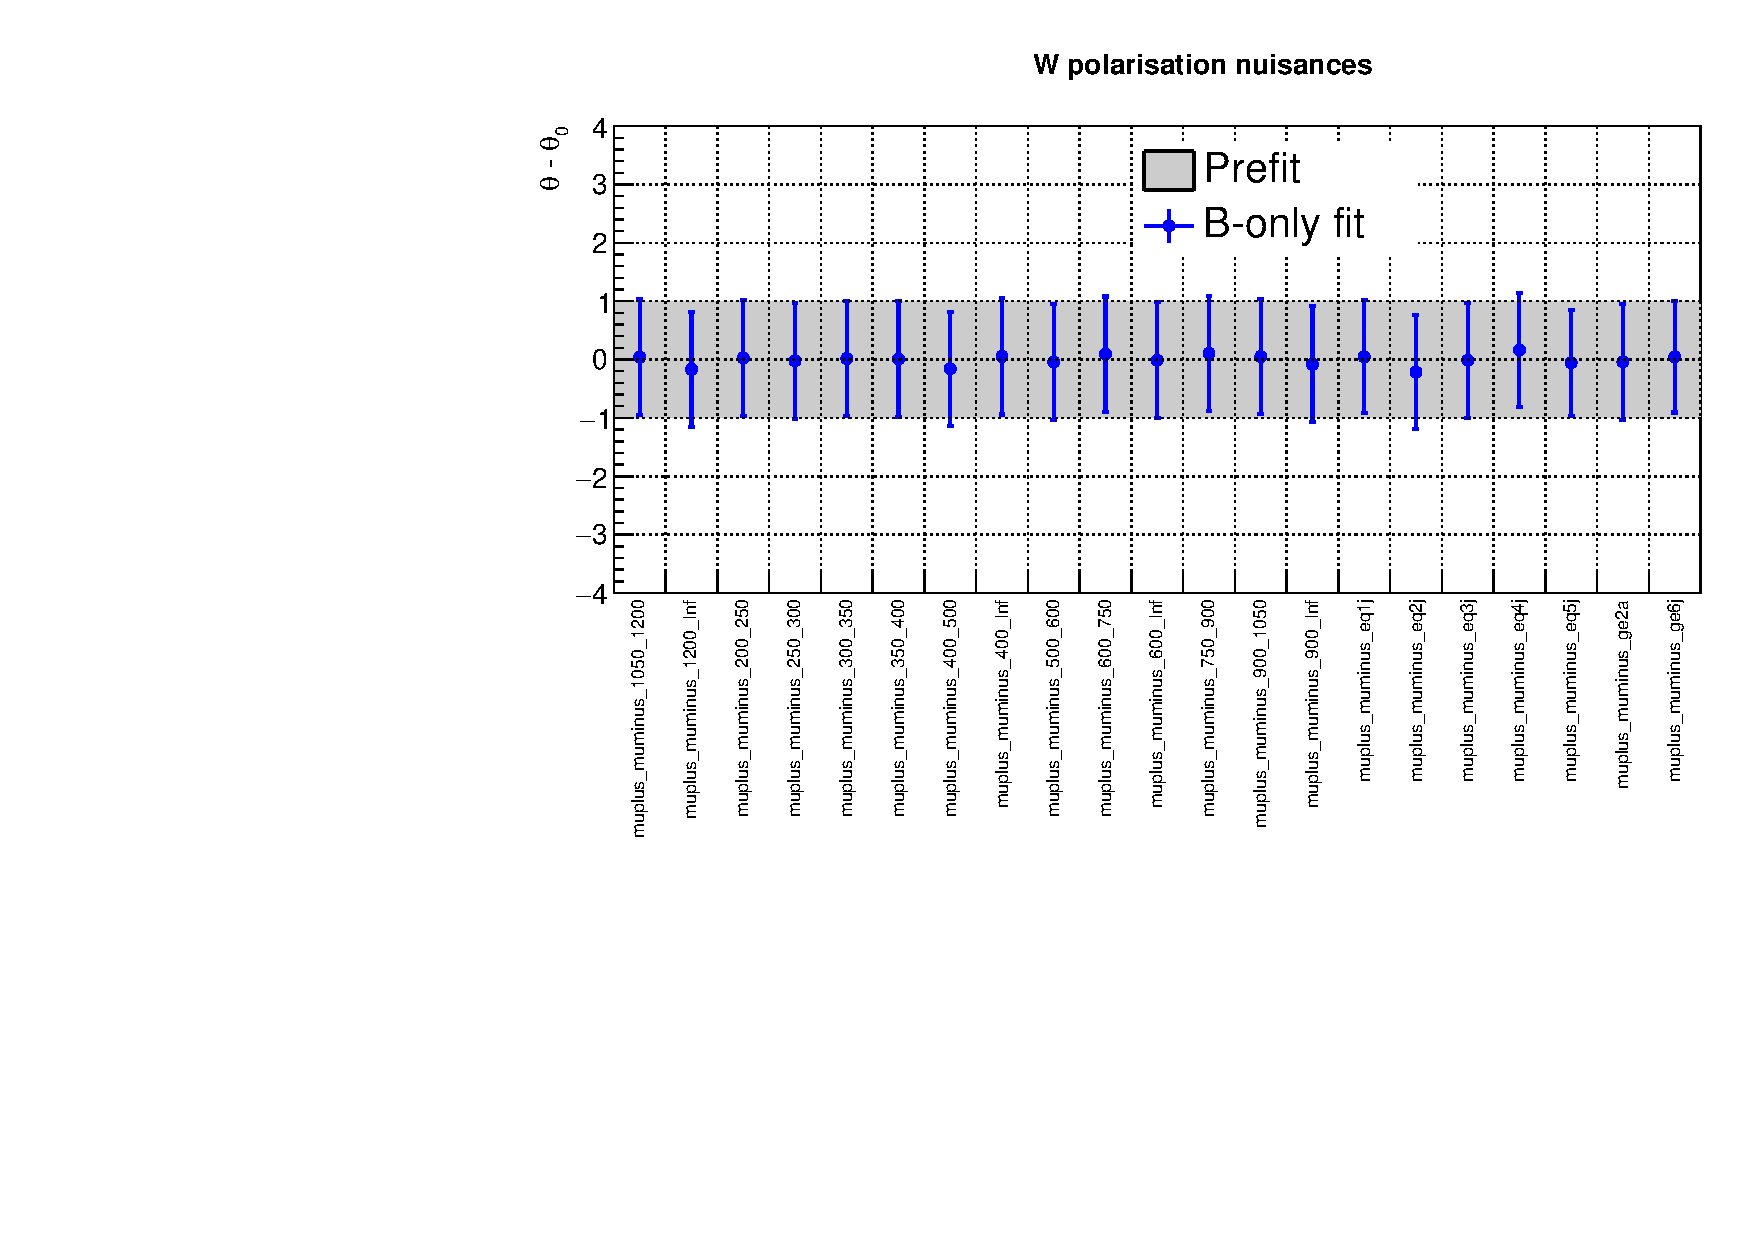
\includegraphics[width=0.8\linewidth]{figures/results/36invfb_preapproval/postfit/nuis/WPol_nuisances}
\end{figure}
